\documentclass[10pt, a4paper]{book}

\usepackage{graphicx}
\def\pdfshellescape{1}
\usepackage{listings}
\usepackage{amsmath}
\usepackage{amsfonts}
\usepackage{longtable}
\usepackage{pgf}

% Gigahertz symbol in math mode, with correct spacing
\newcommand{\GHz}{\,\mathrm{GHz}}
% nanometer symbol
\newcommand{\nm}{\,\mathrm{nm}}
% micron symbol
\newcommand{\micron}{\,\mathrm{\mu m}}
\newcommand{\afmm}{\textsf{afmm}}
\newcommand{\Afmm}{\textsf{Afmm}}


% dB symbol in math mode
\newcommand{\dB}{\,\mathrm{dB}}
% A roman j used for imaginary unit
\newcommand{\junit}{\mathrm{j}}
% Neper constant
\newcommand{\e}{\mathrm{e}}
% It meant to indicate a double bar, but it is too heavy!!!
\newcommand{\dbar}[1]{#1}
% Toeplitz matrix
\newcommand{\indT}{\mathrm{T}}
% Roman indices in mathematical mode
\newcommand{\ped}[1]{_\mathrm{#1}}

\usepackage{xcolor}

\newcommand{\marginpars}[1]{%
  \marginpar{\footnotesize{\it #1}}}

\lstdefinelanguage{AFMM} 
	{morekeywords={size,solve,wavelength, rectangle, substrate, harmonics, pml,inpstruct,outgmodes, lowindex, highindex, indfile, pml_transf, bend, wants,spectrum,propagation,assemble,section,order,excitation,quit,help,
	load, print, select, coefficient, carpet, outdata, matdev, norm, clear, system, goto, label, for, next, eigenvc, eigenam, memocc, symmetry,monitor, power, powerz, let, bloch, outbloch, if, else, endif, size, lg, ln, sin, cos, tan, sqr, abs,arctan,arcsin,arccos,sinh, cosh,tanh,fopen,fclose,
	fprint,addspace,parallel, selmodes, modepos, fscan, fskip, fcheck, do,
	while, angles, indmatrix, parsescript}, 
	sensitive=false,  
	morecomment=[l][\color{blue}]{\#},
} 
\lstset{language=AFMM,%
	basicstyle=\footnotesize\ttfamily,
	keywordstyle=\color{violet}} 


\begin{document}
\title{The \afmm\ 1.4.5 user manual\\[2em]
A 3D full vectorial mode solver and propagator}


\author{Davide Bucci\\[3em] 
\vspace{5em}

\includegraphics[width=6cm]{logo}}

\maketitle
\tableofcontents
\chapter*{Acknowledgments}
I am deeply thankful to Bruno Martin for his friendly help through the detailed comprehension of the Aperiodic Fourier Modal Method. The philosophy of \afmm\ as well as this manual were initially shaped during the frequent discussions we had during the last months of his Ph.D. at IMEP-LAHC, and during his post-doc at IPAG, in Grenoble, France. Alain Morand also participated to intensive comparison sessions with FDTD simulations. 

Another person to whom I am deeply indebted is J\'er\^ome Michallon, who carefully checked all my calculations and corrected several of the mistakes I did. He developed a very detailed understanding of the implementation details, and this allowed him to be active in the code development. Thanks to his work, \afmm\ can now take into account symmetries present in the calculated structure. J\'er\^ome also participated to an accurate revision of this document. Kudos to Elise Ghibaudo; she provided a very detailed feedback and spotted some bugs and errors in this manual.

I would also thank all the colleagues and the students who provided a very welcomed feedback about this software: Thomas Nappez, Marco Casale, Elsa Jardinier, Sandie de Bonnault.

\chapter*{Introduction}
\textsf{
One of the most important things to be considered while studying photonic devices is knowing of their electromagnetic field propagation characteristics. For this reason, several numerical methods have been implemented, in order to study more or less arbitrary wave-guiding or scattering structures. An interesting development is the Aperiodic Fourier Modal Method (AFMM), proposed by Lalanne and Silberstein\cite{lalanne2000fmm,silberstein2001ugt}, in order to apply to waveguides the Rigorous Coupled Wave Method (RCWA), originally developed for the study of diffraction gratings\cite{moharam1981rigorous, li2000recent}. Thanks to the refinements proposed through the years, this method has proven to be effective to treat in a very general way waveguides made with different technologies. It considers structures composed by successive sections of a given length, inside which the refractive index distribution is invariant in the propagation axis. The approach used by the AFMM consists in applying an artificial transverse spatial periodisation to each section. Its effects on the fields are then represented thanks an operator based on a truncated Fourier development and this truncation is the sole approximation done for solving Maxwell equations. Derivatives thus become algebraic operations and the propagation modes are identified as the eigenvectors of a matrix. The complete 3D propagation can finally be studied by imposing the fields continuity conditions at each interface between different sections.}

\textsf{
Afmm is a 3D full vectorial mode solver and propagator based on the Aperiodic Fourier Modal Method. 
The \afmm\ propagator is able to consider the case of straight and bent waveguides, since all the developments can be carried out in rectangular and in cylindrical coordinates as well. It should be noted that, even if the AFMM has  been initially intended for the study of waveguides, the implemented method is quite general and can be used to study diffraction gratings, micro-structured solar cells \cite{el2009photonic} and many other things. 
}

\textsf{
This manual begins with chapter~\ref{chap_implementation}, containing a detailed description of the technical and mathematical background. Even if a comprehension of each detail is probably not needed to use \afmm, it is useful to have a global understanding of the Aperiodic Fourier Modal Method. In fact, the user must clearly know how to cope with the limitations of the method when treating a particular problem.
Chapter~\ref{chap_using} describes how to install and use \afmm\, as well as the  syntax used in the input and output files. A few examples are finally provided, in order to ease the understanding of the structure definition mechanism provided by \afmm.
In the annexes, examples of construction are given for several important matrices used by \afmm\ calculations, the program interaction with Gnuplot is discussed, a description of the file formats used by \afmm , a detailed change-log of this software is given and we list all publications related to \afmm .
}

\chapter{Technical background}
\label{chap_implementation}
\newcommand{\vectorD}[1]{\mathbf{#1}}

\textsf{In this chapter, we present the mathematical development of the Fourier Modal Method in cylindrical coordinates which is the core of \afmm . 
At first, we manipulate Maxwell equations to describe the longitudinal evolution of transverse magnetic and electric fields as the effect of a differential propagation operator. 
We begin by discussing a 2D mode solver, well suited even for bent waveguides having an high core/substrate index contrast. 
We then see how to deal with convergence issues appearing when discontinuities in the refractive index distribution affects the fields for the transverse magnetic (TM) polarisation.
 The Cartesian coordinate calculations can be then seen as a special case of the more general cylindrical coordinates analysis. For this reason, only in a second time we see how the Cartesian coordinates can be treated with a simple limit.
The complete 3D propagation is tackled, via the formalism of the S matrix. We finally extend calculations to Bloch/Floquet modes of periodical structures.
}

\section{Calculation of the transverse fields}
We consider a structure composed by several sections, through which we want to propagate electromagnetic fields. {\em Each section has a refractive index distribution which is invariant along the propagation axis.}\marginpars{What is a structure and a section in \afmm .}
The aim of this paragraph is rewrite curl Maxwell equations in such a way we obtain a (differential) propagation operator which can be applied to the transverse components of the electromagnetic fields in a given section. The developments are done in cylindrical coordinates, following the approach described in~\cite{bucci2012application}.
When the components of the electric and magnetic fields $\vectorD{E}$ and $\vectorD{H}$ have an harmonic time dependance, developing time derivatives can be done in a simple way. First, we consider a structure whose cross section in the propagation direction does not change.
Curl Maxwell equations can thus be written as follows, using the complex representation of $\vectorD{E}$ and $\vectorD{H}$ vectors, in an uncharged dielectric material:
\begin{equation}
\left \{
\begin{aligned}
\nabla \wedge \vectorD{E} &=& -\junit \omega \dbar{\mu} \vectorD{H}
\\
\nabla \wedge \vectorD{H} &=& \junit \omega \dbar{\epsilon} \vectorD{E}
\end{aligned}
\right.
\label{eq_curl_max}
\end{equation}
where $\omega=2\pi f$ and $f$ is the time frequency of the fields,  $\dbar{\epsilon}$ and $\dbar{\mu}$ are respectively the tensors of permittivity and permeability. For simplicity we consider them both diagonal in our analysis, and spatially varying inside the region of interest.
\begin{figure}
\centering
\begin{pgfpicture}{0cm}{0cm}{241pt}{201pt}
% Created by FidoCadJ ver. 0.24, export filter by Davide Bucci
\pgfsetxvec{\pgfpoint{1pt}{0pt}}
\pgfsetyvec{\pgfpoint{0pt}{1pt}}
\pgfsetroundjoin 
\pgfsetroundcap
\pgftranslateto{\pgfxy(0,201)}
\begin{pgfmagnify}{1}{-1}
% Layer color definitions
\definecolor{layer0}{rgb}{0.0,0.0,0.0}
\definecolor{layer1}{rgb}{0.0,0.0,0.0}
\definecolor{layer2}{rgb}{1.0,0.0,0.0}
\definecolor{layer3}{rgb}{0.0,0.5,0.5}
\definecolor{layer4}{rgb}{1.0,0.78,0.0}
\definecolor{layer5}{rgb}{0.5,1.0,0.0}
\definecolor{layer6}{rgb}{0.0,1.0,1.0}
\definecolor{layer7}{rgb}{0.0,0.5,0.0}
\definecolor{layer8}{rgb}{0.6,0.8,0.2}
\definecolor{layer9}{rgb}{1.0,0.08,0.58}
\definecolor{layer10}{rgb}{0.71,0.61,0.05}
\definecolor{layer11}{rgb}{0.0,0.5,1.0}
\definecolor{layer12}{rgb}{0.88,0.88,0.88}
\definecolor{layer13}{rgb}{0.64,0.64,0.64}
\definecolor{layer14}{rgb}{0.37,0.37,0.37}
\definecolor{layer15}{rgb}{0.0,0.0,0.0}
% End of color definitions
\color{layer0}
\pgfsetlinewidth{0.5249999999999999pt}
\pgfline{\pgfxy(41.0,172.0)}{\pgfxy(101.0,112.0)}
\pgfmoveto{\pgfxy(41.0,172.0)}
\pgflineto{\pgfxy(43.121320343559645,168.46446609406726)}
\pgflineto{\pgfxy(44.53553390593274,169.87867965644037)}
\pgfclosepath 
\pgffill 
\pgfline{\pgfxy(71.0,127.0)}{\pgfxy(206.0,127.0)}
\pgfmoveto{\pgfxy(206.0,127.0)}
\pgflineto{\pgfxy(202.0,128.0)}
\pgflineto{\pgfxy(202.0,126.0)}
\pgfclosepath 
\pgffill 
\pgfline{\pgfxy(86.0,150.0)}{\pgfxy(86.0,22.0)}
\pgfmoveto{\pgfxy(86.0,22.0)}
\pgflineto{\pgfxy(87.0,26.0)}
\pgflineto{\pgfxy(85.0,26.0)}
\pgfclosepath 
\pgffill 
\pgfsetdash{{1.0pt}{2.5pt}{2.5pt}{2.5pt}}{0pt}
\pgfline{\pgfxy(86.0,127.0)}{\pgfxy(139.0,150.0)}
\pgfline{\pgfxy(139.0,150.0)}{\pgfxy(139.0,60.0)}
\pgfsetlinewidth{0.33pt}
\pgfcircle[fill]{\pgfxy(139,60)}{1.125pt}\pgfsetlinewidth{0.5249999999999999pt}
\pgfsetdash{}{0pt}
\pgfline{\pgfxy(139.0,60.0)}{\pgfxy(170.0,49.0)}
\pgfmoveto{\pgfxy(170.0,49.0)}
\pgflineto{\pgfxy(166.56469886324578,51.280067126164305)}
\pgflineto{\pgfxy(165.89587917290424,49.39521163520181)}
\pgfclosepath 
\pgffill 
\pgfline{\pgfxy(139.0,60.0)}{\pgfxy(163.0,76.0)}
\pgfmoveto{\pgfxy(163.0,76.0)}
\pgflineto{\pgfxy(159.11709862642337,74.61324950943693)}
\pgflineto{\pgfxy(160.22649901887385,72.94914892076123)}
\pgfclosepath 
\pgffill 
\pgfline{\pgfxy(139.0,60.0)}{\pgfxy(139.0,30.0)}
\pgfmoveto{\pgfxy(139.0,30.0)}
\pgflineto{\pgfxy(140.0,34.0)}
\pgflineto{\pgfxy(138.0,34.0)}
\pgfclosepath 
\pgffill 
\pgfsetdash{{1.0pt}{2.5pt}}{0pt}
\pgfellipse[stroke]{\pgfxy(85.5,36.5)}{\pgfxy(80.5,0)}{\pgfxy(0,30.5)}
\pgfellipse[stroke]{\pgfxy(91.5,125.0)}{\pgfxy(80.5,0)}{\pgfxy(0,31.0)}
\pgfsetlinewidth{0.33pt}
\pgfcircle[fill]{\pgfxy(139,150)}{1.125pt}\pgfsetlinewidth{0.5249999999999999pt}
\pgfmoveto{\pgfxy(77,136)} 
\pgfcurveto{\pgfxy(86,138)}{\pgfxy(97,138)}{\pgfxy(106,136)}
\pgfstroke
\begin{pgfmagnify}{1}{-1}
\pgfputat{\pgfxy(139,-22)}{\pgfbox[left,top]{$\bar{z}$}}
\end{pgfmagnify}
\begin{pgfmagnify}{1}{-1}
\pgfputat{\pgfxy(175,-43)}{\pgfbox[left,top]{$\bar{\theta}$}}
\end{pgfmagnify}
\begin{pgfmagnify}{1}{-1}
\pgfputat{\pgfxy(166,-76)}{\pgfbox[left,top]{$\bar{r}$}}
\end{pgfmagnify}
\begin{pgfmagnify}{1}{-1}
\pgfputat{\pgfxy(143,-90)}{\pgfbox[left,top]{$z$}}
\end{pgfmagnify}
\begin{pgfmagnify}{1}{-1}
\pgfputat{\pgfxy(209,-126)}{\pgfbox[left,top]{$y$}}
\end{pgfmagnify}
\begin{pgfmagnify}{1}{-1}
\pgfputat{\pgfxy(35,-174)}{\pgfbox[left,top]{$x$}}
\end{pgfmagnify}
\begin{pgfmagnify}{1}{-1}
\pgfputat{\pgfxy(83,-15)}{\pgfbox[left,top]{$z$}}
\end{pgfmagnify}
\begin{pgfmagnify}{1}{-1}
\pgfputat{\pgfxy(76,-141)}{\pgfbox[left,top]{$\theta$}}
\end{pgfmagnify}
\begin{pgfmagnify}{1}{-1}
\pgfputat{\pgfxy(118,-135)}{\pgfbox[left,top]{$r$}}
\end{pgfmagnify}
\end{pgfmagnify}
\end{pgfpicture}
\caption{The cylindrical coordinate system.}
\label{fig_cyl_coordinates}
\end{figure}
Considering the cylindrical coordinate system shown in figure~\ref{fig_cyl_coordinates}, we consider that the propagation axis is $\theta$. Separating the $r$, $z$ and $\theta$ components in equations \eqref{eq_curl_max}, we obtain what follows:
\begin{equation}
\left \{
\begin{aligned}
\frac{1}{r}\frac{\partial E_z}{\partial \theta}-\frac{\partial E_\theta}{\partial z}&=&-\mu_r\junit\omega H_r
\\
\frac{\partial E_r}{\partial z}-\frac{\partial E_z}{\partial r}&=&-\mu_\theta\junit\omega H_\theta
\\
\frac{1}{r}\left(\frac{\partial(r E_\theta)}{\partial r}-\frac{\partial E_r}{\partial \theta}\right)&=&-\mu_z\junit\omega H_z
\\
\frac{1}{r}\frac{\partial H_z}{\partial \theta}-\frac{\partial H_\theta}{\partial z}&=&\epsilon_r\junit\omega E_r
\\
\frac{\partial H_r}{\partial z}-\frac{\partial H_z}{\partial r}&=&\epsilon_\theta\junit\omega E_\theta
\\
\frac{1}{r}\left(\frac{\partial(r H_\theta)}{\partial r}-\frac{\partial H_r}{\partial \theta}\right)&=&\epsilon_z\junit\omega E_z
\end{aligned}
\right.
\label{eq_fields_components}
\end{equation}

Each one of the sections composing the structure must have the bending radius and the transverse distribution of the refractive index invariant along the propagation axis $\theta$. We notice that the radial coordinate $r$ appears in equations \eqref{eq_fields_components} and it is a spatially variable term. This implies that it should be treated in the same way as the other spatially variable terms, such as the permeabilities and permittivities.

The terms $H_\theta$ and $E_\theta$ can be extracted from equations \eqref{eq_fields_components}  and injected again in the remaining expressions, to obtain a system of only 4 equations instead of 6, which describe the behaviour of the fields components transverse to the propagation axis ($E_r$, $E_z$, $H_r$ and $H_z$). Those equations constitute a propagation operator giving the evolution of the fields while propagation. 
Regrouping in the first member the derivatives calculated with respect to $\theta$ yields the following equations:
\begin{equation}
\left \{
\begin{aligned}
\frac{\partial E_r}{\partial \theta} &=& \frac{\partial}{\partial r}\left [ \frac{r}{\junit \omega \epsilon_\theta}\left(\frac{\partial H_r}{\partial z} - \frac{\partial H_z}{\partial r}\right)\right]+\junit\omega\mu_z r H_z 
\\
\frac{\partial E_z}{\partial \theta} &=& r\frac{\partial}{\partial z}\left [ \frac{1}{\junit \omega \epsilon_\theta}\left(\frac{\partial H_r}{\partial z} - \frac{\partial H_z}{\partial r}\right)\right]-\junit\omega\mu_r r H_r 
\\
\frac{\partial H_r}{\partial \theta} &=& \frac{\partial}{\partial r}\left [ -\frac{r}{\junit \omega \mu_\theta}\left(\frac{\partial E_r}{\partial z} - \frac{\partial E_z}{\partial r}\right)\right]-\junit\omega\epsilon_z r E_z
\\
\frac{\partial H_z}{\partial \theta} &=& r\frac{\partial}{\partial z}\left [ -\frac{1}{\junit \omega \mu_\theta}\left(\frac{\partial E_r}{\partial z} - \frac{\partial E_z}{\partial r}\right)\right]+\junit\omega\epsilon_r r E_r.
\end{aligned}
\right. 
\label{eq_propag_cyl}
\end{equation}
Those equations may be used in this form, or alternatively some derivatives may be developed further, in this way:
{\footnotesize
\begin{equation}
\left \{
\begin{aligned}
\frac{\partial E_r}{\partial \theta} = \junit \omega\mu_z r H_z + \frac{1}{\junit \omega}\frac{1}{\epsilon_\theta}\left (\frac{\partial H_r}{\partial z}-\frac{\partial H_z}{\partial r}\right)+\frac{1}{\junit \omega}r\frac{\partial}{\partial r}\left (\frac{1}{\epsilon_\theta}\right)\left(\frac{\partial H_r}{\partial z}-\frac{\partial H_z}{\partial r}\right)+\\
+\frac{1}{\junit \omega}\frac{r}{\epsilon_\theta}\left( \frac{\partial^2 H_r}{\partial r\partial z}-\frac{\partial^2 H_z}{\partial r^2}\right)\\
%
\frac{\partial E_z}{\partial \theta} = -\junit \omega\mu_r r H_r + \frac{1}{\junit \omega}r \frac{\partial}{\partial z}\left(\frac{1}{\epsilon_\theta}\right)\left (\frac{\partial H_r}{\partial z}-\frac{\partial H_z}{\partial r}\right)+\frac{1}{\junit \omega}r \frac{1}{\epsilon_\theta}\left( \frac{\partial^2 H_r}{\partial z^2}-\frac{\partial^2 H_z}{\partial z\partial r}\right)\\
%
\frac{\partial H_r}{\partial \theta} =- \junit \omega\epsilon_z r E_z - \frac{1}{\junit \omega}\frac{1}{\mu_\theta}\left (\frac{\partial E_r}{\partial z}-\frac{\partial E_z}{\partial r}\right)-\frac{1}{\junit \omega}r\frac{\partial}{\partial r}\left (\frac{1}{\mu_\theta}\right)\left(\frac{\partial E_r}{\partial z}-\frac{\partial E_z}{\partial r}\right)+\\
-\frac{1}{\junit \omega}\frac{r}{\mu_\theta}\left( \frac{\partial^2 E_r}{\partial r\partial z}-\frac{\partial^2 E_z}{\partial r^2}\right)\\
%
\frac{\partial H_z}{\partial \theta} = -\junit \omega\epsilon_r r E_r - \frac{1}{\junit \omega}r \frac{\partial}{\partial z}\left(\frac{1}{\mu_\theta}\right)\left (\frac{\partial E_r}{\partial z}-\frac{\partial E_z}{\partial r}\right)-\frac{1}{\junit \omega}r \frac{1}{\mu_\theta}\left( \frac{\partial^2 E_r}{\partial z^2}-\frac{\partial^2 E_z}{\partial z\partial r}\right)
\end{aligned}
\right.
\label{eq_propag_cyl_dev}
\end{equation}}

In this context, a propagation mode might be seen as a configuration of the electromagnetic field propagating without changing its shape, but {\em it can also be seen as an eigenfunction of the differential operator described by equations~\eqref{eq_propag_cyl}}. \marginpars{What is a mode in \afmm .} We try to represent fields via a base constituted by eigenfunctions, whose propagation is therefore relatively simple to being taken into account. Before doing that, we must represent all fields and spatially varying terms in a convenient way to perform algebraic calculations instead of calculating space derivatives. This can be done by exploiting the properties of the Fourier series, as it is described in the next paragraphs. 

\section{Fourier series field development}
\label{sec_periodization}
\subsection{Developing terms}
\begin{figure}
\centering
\footnotesize
\begin{pgfpicture}{0cm}{0cm}{261pt}{135pt}
% Created by FidoCadJ ver. 0.23.4 alpha, export filter by Davide Bucci
\pgfsetxvec{\pgfpoint{1pt}{0pt}}
\pgfsetyvec{\pgfpoint{0pt}{1pt}}
\pgfsetroundjoin 
\pgfsetroundcap
\pgftranslateto{\pgfxy(0,135)}
\begin{pgfmagnify}{1}{-1}
% Layer color definitions
\definecolor{layer0}{rgb}{0.0,0.0,0.0}
\definecolor{layer1}{rgb}{0.0,0.0,0.5}
\definecolor{layer2}{rgb}{1.0,0.0,0.0}
\definecolor{layer3}{rgb}{0.0,0.5,0.5}
\definecolor{layer4}{rgb}{0.54,0.82,0.57}
\definecolor{layer5}{rgb}{0.0,0.0,0.0}
\definecolor{layer6}{rgb}{1.0,1.0,1.0}
\definecolor{layer7}{rgb}{1.0,0.78,0.0}
\definecolor{layer8}{rgb}{1.0,0.78,0.0}
\definecolor{layer9}{rgb}{1.0,0.78,0.0}
\definecolor{layer10}{rgb}{1.0,0.78,0.0}
\definecolor{layer11}{rgb}{1.0,0.78,0.0}
\definecolor{layer12}{rgb}{1.0,0.78,0.0}
\definecolor{layer13}{rgb}{1.0,0.78,0.0}
\definecolor{layer14}{rgb}{0.0,0.0,0.0}
\definecolor{layer15}{rgb}{0.0,0.0,0.0}
% End of color definitions
\color{layer0}
\begin{pgfmagnify}{1}{-1}
\pgfputat{\pgfxy(13,-29)}{\pgfbox[left,top]{$y$}}
\end{pgfmagnify}
\begin{pgfmagnify}{1}{-1}
\pgfputat{\pgfxy(147,-119)}{\pgfbox[left,top]{$x$}}
\end{pgfmagnify}
\begin{pgfmagnify}{1}{-1}
\pgfputat{\pgfxy(17,-124)}{\pgfbox[left,top]{$z$}}
\end{pgfmagnify}
\begin{pgfmagnify}{1}{-1}
\pgfputat{\pgfxy(112,-104)}{\pgfbox[left,top]{$z$}}
\end{pgfmagnify}
\begin{pgfmagnify}{1}{-1}
\pgfputat{\pgfxy(108,-9)}{\pgfbox[left,top]{$y$}}
\end{pgfmagnify}
\begin{pgfmagnify}{1}{-1}
\pgfputat{\pgfxy(252,-99)}{\pgfbox[left,top]{$x$}}
\end{pgfmagnify}
\begin{pgfmagnify}{1}{-1}
\pgfputat{\pgfxy(143,-76)}{\pgfbox[left,top]{$n_g$}}
\end{pgfmagnify}
\begin{pgfmagnify}{1}{-1}
\pgfputat{\pgfxy(121,-65)}{\pgfbox[left,top]{$n_0$}}
\end{pgfmagnify}
\begin{pgfmagnify}{1}{-1}
\pgfputat{\pgfxy(40,-110)}{\pgfbox[left,top]{Structure}}
\end{pgfmagnify}
\begin{pgfmagnify}{1}{-1}
\pgfputat{\pgfxy(26,-85)}{\pgfbox[left,top]{$n_0$}}
\end{pgfmagnify}
\begin{pgfmagnify}{1}{-1}
\pgfputat{\pgfxy(48,-96)}{\pgfbox[left,top]{$n_g$}}
\end{pgfmagnify}
\begin{pgfmagnify}{1}{-1}
\pgfputat{\pgfxy(186,-65)}{\pgfbox[left,top]{$n_0$}}
\end{pgfmagnify}
\begin{pgfmagnify}{1}{-1}
\pgfputat{\pgfxy(208,-76)}{\pgfbox[left,top]{$n_g$}}
\end{pgfmagnify}
\begin{pgfmagnify}{1}{-1}
\pgfputat{\pgfxy(121,-25)}{\pgfbox[left,top]{$n_0$}}
\end{pgfmagnify}
\begin{pgfmagnify}{1}{-1}
\pgfputat{\pgfxy(143,-36)}{\pgfbox[left,top]{$n_g$}}
\end{pgfmagnify}
\begin{pgfmagnify}{1}{-1}
\pgfputat{\pgfxy(186,-25)}{\pgfbox[left,top]{$n_0$}}
\end{pgfmagnify}
\begin{pgfmagnify}{1}{-1}
\pgfputat{\pgfxy(208,-36)}{\pgfbox[left,top]{$n_g$}}
\end{pgfmagnify}
\begin{pgfmagnify}{1}{-1}
\pgfputat{\pgfxy(172,-101)}{\pgfbox[left,top]{$T_x$}}
\end{pgfmagnify}
\begin{pgfmagnify}{1}{-1}
\pgfputat{\pgfxy(100,-54)}{\pgfbox[left,top]{$T_y$}}
\end{pgfmagnify}
\color{layer1}
\pgfsetlinewidth{0.5pt}
\pgfmoveto{\pgfxy(218,71)} 
\pgfcurveto{\pgfxy(208,66)}{\pgfxy(198,71)}{\pgfxy(203,86)}
\pgfstroke
\pgfmoveto{\pgfxy(138,46)} 
\pgfcurveto{\pgfxy(143,56)}{\pgfxy(163,36)}{\pgfxy(153,31)}
\pgfstroke
\pgfmoveto{\pgfxy(203,46)} 
\pgfcurveto{\pgfxy(208,56)}{\pgfxy(228,36)}{\pgfxy(218,31)}
\pgfstroke
\pgfmoveto{\pgfxy(43,106)} 
\pgfcurveto{\pgfxy(48,116)}{\pgfxy(68,96)}{\pgfxy(58,91)}
\pgfstroke
\pgfmoveto{\pgfxy(153,71)} 
\pgfcurveto{\pgfxy(143,66)}{\pgfxy(133,71)}{\pgfxy(138,86)}
\pgfstroke
\pgfmoveto{\pgfxy(218,31)} 
\pgfcurveto{\pgfxy(208,26)}{\pgfxy(198,31)}{\pgfxy(203,46)}
\pgfstroke
\pgfmoveto{\pgfxy(203,86)} 
\pgfcurveto{\pgfxy(208,96)}{\pgfxy(228,76)}{\pgfxy(218,71)}
\pgfstroke
\pgfmoveto{\pgfxy(138,86)} 
\pgfcurveto{\pgfxy(143,96)}{\pgfxy(163,76)}{\pgfxy(153,71)}
\pgfstroke
\pgfmoveto{\pgfxy(153,31)} 
\pgfcurveto{\pgfxy(143,26)}{\pgfxy(133,31)}{\pgfxy(138,46)}
\pgfstroke
\pgfmoveto{\pgfxy(58,91)} 
\pgfcurveto{\pgfxy(48,86)}{\pgfxy(38,91)}{\pgfxy(43,106)}
\pgfstroke
\color{layer4}
\pgfsetdash{{1.0pt}{2.5pt}}{0pt}
\pgfline{\pgfxy(110,100)}{\pgfxy(79,106)}
\pgfline{\pgfxy(80,80)}{\pgfxy(175,60)}
\pgfline{\pgfxy(15,80)}{\pgfxy(110,60)}
\pgfline{\pgfxy(80,120)}{\pgfxy(175,100)}
\color{layer5}
\pgfsetdash{}{0pt}
\pgfline{\pgfxy(5,120)}{\pgfxy(145,120)}
\pgfmoveto{\pgfxy(145,120)}
\pgflineto{\pgfxy(142.0,121.0)}
\pgflineto{\pgfxy(142.0,119.0)}
\pgfclosepath 
\pgffill 
\pgfline{\pgfxy(110,115)}{\pgfxy(110,15)}
\pgfmoveto{\pgfxy(110,15)}
\pgflineto{\pgfxy(111.0,18.0)}
\pgflineto{\pgfxy(109.0,18.0)}
\pgfclosepath 
\pgffill 
\pgfline{\pgfxy(100,100)}{\pgfxy(250,100)}
\pgfmoveto{\pgfxy(250,100)}
\pgflineto{\pgfxy(247.0,101.0)}
\pgflineto{\pgfxy(247.0,99.0)}
\pgfclosepath 
\pgffill 
\pgfmoveto{\pgfxy(110,20)}
\pgflineto{\pgfxy(175,20)}
\pgflineto{\pgfxy(175,60)}
\pgflineto{\pgfxy(110,60)}
\pgfclosepath 
\pgfqstroke 
\pgfline{\pgfxy(15,135)}{\pgfxy(15,35)}
\pgfmoveto{\pgfxy(15,35)}
\pgflineto{\pgfxy(16.0,38.0)}
\pgflineto{\pgfxy(14.0,38.0)}
\pgfclosepath 
\pgffill 
\pgfmoveto{\pgfxy(175,60)}
\pgflineto{\pgfxy(240,60)}
\pgflineto{\pgfxy(240,100)}
\pgflineto{\pgfxy(175,100)}
\pgfclosepath 
\pgfqstroke 
\pgfmoveto{\pgfxy(15,80)}
\pgflineto{\pgfxy(80,80)}
\pgflineto{\pgfxy(80,120)}
\pgflineto{\pgfxy(15,120)}
\pgfclosepath 
\pgfqstroke 
\pgfmoveto{\pgfxy(110,60)}
\pgflineto{\pgfxy(175,60)}
\pgflineto{\pgfxy(175,100)}
\pgflineto{\pgfxy(110,100)}
\pgfclosepath 
\pgfqstroke 
\pgfmoveto{\pgfxy(175,20)}
\pgflineto{\pgfxy(240,20)}
\pgflineto{\pgfxy(240,60)}
\pgflineto{\pgfxy(175,60)}
\pgfclosepath 
\pgfqstroke 
\color{layer6}
\pgfellipse[fillstroke]{\pgfxy(110.0,100.0)}{\pgfxy(3.0,0)}{\pgfxy(0,3.0)}
\pgfellipse[fillstroke]{\pgfxy(15.0,120.0)}{\pgfxy(3.0,0)}{\pgfxy(0,3.0)}
\color{layer14}
\pgfellipse[stroke]{\pgfxy(110.0,100.0)}{\pgfxy(3.0,0)}{\pgfxy(0,3.0)}
\pgfellipse[stroke]{\pgfxy(15.0,120.0)}{\pgfxy(3.0,0)}{\pgfxy(0,3.0)}
\pgfsetlinewidth{0.33pt}
\pgfcircle[fill]{\pgfxy(110,100)}{1.0pt}\pgfcircle[fill]{\pgfxy(15,120)}{1.0pt}\end{pgfmagnify}
\end{pgfpicture}
\caption{The periodization technique applied to develop the permittivity and permeability in Fourier series.}
\label{fig_periodisation}
\end{figure}
\begin{figure}
\centering
\begin{pgfpicture}{0cm}{0cm}{386pt}{180pt}
% Created by FidoCadJ ver. 0.23.4 alpha, export filter by Davide Bucci
\pgfsetxvec{\pgfpoint{2pt}{0pt}}
\pgfsetyvec{\pgfpoint{0pt}{2pt}}
\pgfsetroundjoin 
\pgfsetroundcap
\pgftranslateto{\pgfxy(0,90)}
\begin{pgfmagnify}{1}{-1}
% Layer color definitions
\definecolor{layer0}{rgb}{0.54,0.82,0.57}
\definecolor{layer1}{rgb}{0.0,0.0,0.0}
\definecolor{layer2}{rgb}{1.0,0.0,0.0}
\definecolor{layer3}{rgb}{0.0,0.5,0.5}
\definecolor{layer4}{rgb}{1.0,0.78,0.0}
\definecolor{layer5}{rgb}{1.0,0.78,0.0}
\definecolor{layer6}{rgb}{1.0,0.78,0.0}
\definecolor{layer7}{rgb}{1.0,0.78,0.0}
\definecolor{layer8}{rgb}{1.0,0.78,0.0}
\definecolor{layer9}{rgb}{1.0,0.78,0.0}
\definecolor{layer10}{rgb}{1.0,0.78,0.0}
\definecolor{layer11}{rgb}{1.0,0.78,0.0}
\definecolor{layer12}{rgb}{1.0,0.78,0.0}
\definecolor{layer13}{rgb}{1.0,0.78,0.0}
\definecolor{layer14}{rgb}{0.0,0.0,0.0}
\definecolor{layer15}{rgb}{0.0,0.0,0.0}
% End of color definitions
\color{layer0}
\pgfsetlinewidth{1.0pt}
\pgfsetdash{{1.0pt}{2.5pt}}{0pt}
\pgfline{\pgfxy(10,20)}{\pgfxy(125,20)}
\pgfline{\pgfxy(10,70)}{\pgfxy(125,70)}
\pgfline{\pgfxy(65,15)}{\pgfxy(65,80)}
\pgfline{\pgfxy(115,15)}{\pgfxy(115,80)}
\pgfline{\pgfxy(10,45)}{\pgfxy(125,45)}
\pgfline{\pgfxy(15,15)}{\pgfxy(15,80)}
\color{layer1}
\begin{pgfmagnify}{1}{-1}
\pgfputat{\pgfxy(100,-85)}{\pgfbox[left,top]{$r\ped{p}$, periodicized radius}}
\end{pgfmagnify}
\pgfsetdash{}{0pt}
\pgfline{\pgfxy(65,70)}{\pgfxy(115,20)}
\pgfline{\pgfxy(15,20)}{\pgfxy(5,30)}
\pgfline{\pgfxy(115,70)}{\pgfxy(125,60)}
\begin{pgfmagnify}{1}{-1}
\pgfputat{\pgfxy(30,-5)}{\pgfbox[left,top]{radius $r$}}
\end{pgfmagnify}
\pgfline{\pgfxy(10,80)}{\pgfxy(135,80)}
\pgfmoveto{\pgfxy(135,80)}
\pgflineto{\pgfxy(132.0,81.0)}
\pgflineto{\pgfxy(132.0,79.0)}
\pgfclosepath 
\pgffill 
\pgfline{\pgfxy(15,70)}{\pgfxy(65,20)}
\pgfline{\pgfxy(40,85)}{\pgfxy(40,10)}
\pgfmoveto{\pgfxy(40,10)}
\pgflineto{\pgfxy(41.0,13.0)}
\pgflineto{\pgfxy(39.0,13.0)}
\pgfclosepath 
\pgffill 
\begin{pgfmagnify}{1}{-1}
\pgfputat{\pgfxy(60,-85)}{\pgfbox[left,top]{$\frac{T_r}{2}$}}
\end{pgfmagnify}
\begin{pgfmagnify}{1}{-1}
\pgfputat{\pgfxy(10,-85)}{\pgfbox[left,top]{$-\frac{T_r}{2}$}}
\end{pgfmagnify}
\begin{pgfmagnify}{1}{-1}
\pgfputat{\pgfxy(35,-40)}{\pgfbox[left,top]{$r_0$}}
\end{pgfmagnify}
\begin{pgfmagnify}{1}{-1}
\pgfputat{\pgfxy(30,-65)}{\pgfbox[left,top]{$r\ped{min}$}}
\end{pgfmagnify}
\begin{pgfmagnify}{1}{-1}
\pgfputat{\pgfxy(29,-15)}{\pgfbox[left,top]{$r\ped{max}$}}
\end{pgfmagnify}
\end{pgfmagnify}
\end{pgfpicture}
\caption{The effect of the periodization on the radius: it becomes a sawtooth.}
\label{fig_periodicized_r}
\end{figure}

The Fourier Modal Method is based on the {\em application of a periodization of the transverse permeability, permittivity and field distributions, by replicating a chosen calculation window, whose span is $T_r$ and $T_z$ in the $r$ and $z$ directions.} \marginpars{Fourier series and \afmm .}
This is represented schematically in figure~\ref{fig_periodisation} and allows to describe each spatially varying term by means of Fourier series.
Of course, this may give an infinite number of terms to be considered for solving equation~\eqref{eq_propag_cyl}.

By taking into account only $2S_r-1$ complex Fourier coefficients in the $r$ axis and $2S_z-1$ in the $z$ axis, the expansion is truncated to a finite number of harmonics. \marginpars{Truncation.}
Taking for example $\epsilon_r$, the $r$ component of the permittivity, we can write:
\begin{equation}
\epsilon_r(r,z) = \sum_{m=-(S_r-1)}^{S_r-1} \sum_{n=-(S_z-1)}^{S_z-1} P_{m,n}\e^{\junit(m\nu_r r+ n\nu_z z)},
\label{eq_epsilon_series}
\end{equation}
where $\nu_r=2\pi / T_r$ is the fundamental spatial frequency on the $r$ axis, $\nu_z=2\pi / T_z$ is the fundamental space frequency on the $z$ axis and $P_{m,n}$ is the $m$-order along $r$ and $n$-order along $z$ Fourier coefficient of the $\epsilon_r$ expansion.

In the same way, by developing in complex Fourier series all space variable terms of equations~\eqref{eq_propag_cyl}, over the periods $T_r=1/\nu_r$ and $T_z=1/\nu_z$:
\begin{equation}
E_r=\sum_{a_r}\sum_{a_z} A_{a_r,a_z} \e^{\junit (a_r \nu_r r+a_z \nu_z z)}
\end{equation}
\begin{equation}
E_z=\sum_{b_r}\sum_{b_z} B_{b_r,b_z} \e^{\junit (b_r \nu_r r+b_z \nu_z z)}
\end{equation}
\begin{equation}
H_r=\sum_{c_r}\sum_{c_z} C_{c_r,c_z} \e^{\junit (c_r \nu_r r+c_z \nu_z z)}
\label{eq_fourier_dev_hz}
\end{equation}
\begin{equation}
H_z=\sum_{d_r}\sum_{d_z} D_{d_r,d_z} \e^{\junit (d_r \nu_r r+d_z \nu_z z)}
\end{equation}
%
\begin{equation}
\mu_r=\sum_{m_r}\sum_{m_z} M_{m_r,m_z} \e^{\junit (m_r \nu_r r+m_z \nu_z z)}
\end{equation}
\begin{equation}
\mu_z=\sum_{n_r}\sum_{n_z} N_{n_r,n_z} \e^{\junit (n_r \nu_r r+n_z \nu_z z)}
\end{equation}
\begin{equation}
\frac{1}{\mu_\theta}=\sum_{o_r}\sum_{o_z} O_{o_r,o_z} \e^{\junit (o_r \nu_r r+o_z \nu_z z)}
\end{equation}
%
\begin{equation}
\epsilon_r=\sum_{p_r}\sum_{p_z} P_{p_r,p_z} \e^{\junit (p_r \nu_r r+p_z \nu_z z)}
\end{equation}
\begin{equation}
\epsilon_z=\sum_{q_r}\sum_{q_z} Q_{q_r,q_z} \e^{\junit (q_r \nu_r r+q_z \nu_z z)}
\end{equation}
\begin{equation}
\frac{1}{\epsilon_\theta}=\sum_{r_r}\sum_{r_z} R_{r_r,r_z} \e^{\junit (r_r \nu_r r+r_z \nu_z z)}
\end{equation}
Here, symbols $A$, $B$, $C$ and $D$ represent the complex amplitudes of the transverse electric and magnetic fields, while $M$, $N$, $O$, $P$, $Q$ and $R$ are related to the permeability and permittivity. 

Thanks to the artificial periodisation, the evolution of the radial coordinate $r\ped{p}(r)$ appears to be a sawtooth wave, as shown in figure~\ref{fig_periodicized_r}. Its Fourier $m$-th order term $r_m$ can hence be analytically calculated as follows:
\begin{equation}
r_m=
\begin{cases}
r_0 & \text{if $m=0$,}\\
\junit\frac{T_r}{2\pi m} & \text{if $m\ne 0$.}
\end{cases}
\label{eq_radius_develop}
\end{equation}
where $r_0$ and $T_r$ are respectively the bending radius of the centre and the total size in $r$ of the calculation window. 


Considering as usual $\theta$ as propagation axis, the modal fields have a  dependance on $\theta$ on the form $\exp ( -\junit \beta\ped{s} \theta)$, where $\beta\ped{s} $ is unknown and should be determined. This is advantageous to calculate all the partial derivatives with respect to $\theta$ appearing in equation~\ref{eq_propag_cyl}. Equations~\eqref{eq_propag_cyl} being linear, it is possible to exploit that with Fourier series, and translate equations term by term into matrix operations in the Fourier space. The goal of the following paragraphs will be to write equations~\eqref{eq_propag_cyl} as an operator applicable to the fields as a matrix vector multiplication.

\subsection{Convolutions}
\label{subsec_convolution}
In equations~\eqref{eq_propag_cyl}, written in the spatial domain, some terms  contain a product between space-varying quantities. If we consider the last part of the very first equation:
\begin{equation}
\mathrm{j}\omega \mu_z r H_z,
\label{eq_space_product_term}
\end{equation}
the $\mathrm{j}\omega$ does not pose any problem, since it is a constant (the wavelength at which the calculation is done, hence $\omega$, is chosen at the very beginning). More complex is the product between $\mu$, $r$ and $H_z$, since all those terms are space-varying. The well-known convolution theorem states that they must be handled with convolutions in the Fourier domain. Hence, the problem is knowing how to translate that into convenient matrix operations.

Let us in particular focus on how the product $r$ times $H_z$ may be written. The first thing to do is calculate the Fourier coefficients for $r$, from equation~\eqref{eq_radius_develop}. Then, we arrange them in a block-Toeplitz matrix which we will call $S\ped{T}$, constructed with the rules shown in equations~\eqref{eq_block_toeplitz1} and \eqref{eq_block_toeplitz2}, as described in paragraph~\ref{sec_toeplitz}. At the same time, the harmonics $D_{dr,dz}$ constituting the $z$ component of the magnetic field (still unknown, for the moment) are arranged\footnote{Packing them into a usable column vector is a little tricky. Details are given in paragraph~\ref{sec_toeplitz} in Appendix~\ref{chap_matrix_examples}.} in a column vector which will be called $[H_z]$.
It can be shown that the convolution corresponding to the two last terms of equation~\eqref{eq_space_product_term} is written as follows in the Fourier domain:
\begin{equation}
S\ped{T}[H_z]
\end{equation}
More complicated is now to consider the double convolution resulting by the presence of a $\mu_z$. If possible, the product $\mu_z r$ can be calculated in the spatial domain, before taking the Fourier transform of the result. In some cases, however, an approximate result of the convolution can be conveniently written directly in the Fourier domain, in the following way:
\begin{equation}
\junit \omega N\ped{T}S\ped{T}[H_x].
\end{equation}
In other words, the convolution between coefficients for representing $\mu_z$ and $r$ is translated (quite brutally, indeed, as this is only asymptotically true \cite{gray2006toeplitz}) into a product of Block-Toeplitz matrix. If this strategy is adopted, the matrix product being non commutative, there is not an unique way to write matrix order. For this and other more subtile reasons presented below, \afmm\ offers a choice of different strategies via the \lstinline!matdev! command.

\subsection{Derivatives}
\label{subsec_derivatives}
The reason for which each space-varying term has been represented as a Fourier series is that derivatives are translated into a purely algebrical operator.
Let us consider the following derivative:
\begin{equation}
\frac{\partial H_r}{\partial z},
\end{equation}
which can be thought as a differential operator applied to the $H_z$ component of the field. In Fourier developments, it is well known that taking the derivatives translates into a multiplication with a frequency term. If $D_{d_r, d_z}$ is the term corresponding to the $d_r$ harmonics in $r$ and $d_z$ harmonics in $z$ (see equation~\eqref{eq_fourier_dev_hz}), the corresponding term of the $r$ derivative of $H_z$ is $\junit d_r\nu_r D_{d_r, d_z}$.
The situation becomes more intricate when dealing with terms which are more complicated.

Two different strategies are applied in \afmm :

\begin{itemize}
\item The one which is a legacy of the beginnings consists in preparing appropriate bloc-matrices containing the derivative terms ($ d_r\nu_r$) and perform Hadamard multiplications (term by term, not line by column) with the other terms needing to be derived. Considering the propagation operator in the developed form, from equation \eqref{eq_propag_cyl_dev}, we have terms such as the following:
\begin{equation}
\frac{1}{\junit\omega} \frac{\partial}{\partial r}\left(\frac{1}{\epsilon_\theta}\right)\frac{\partial H_r}{\partial z}.
\end{equation}
A convolution is represented between the terms coming from the development of $r$, the derivative of $\epsilon_\theta^{-1}$ and the $z$ derivative of $H_r$. In matrix form, this may be written with a modified-Toeplitz matrix formalism, as follows\footnote{The modified-Toeplitz formalism has been invented during the development of \afmm\ and it is used in \cite{bucci2010study}. No one seems to understand it and it is undeniably heavy. The description is still in this document, because of the traces it has left in the source code. In the future, we will probably work more with the compact matrix notation which is commonly found in the literature\dots}:
\begin{equation}
-\frac{1}{\junit\omega}R_{\mathrm{T},r}^{(z)}[H_z].
\end{equation}
The minus sign comes from the two multiplications by the imaginary unit $\junit$ coming out from the derivatives. All terms can be written using this notation. For example:
\begin{equation}
\frac{1}{\junit\omega\epsilon_\theta}\frac{\partial^2 H_r}{\partial z^2} \leftrightarrow   -\frac{1}{\junit\omega}R_{\mathrm{T}}^{(zz)}[H_r],
\end{equation}
\begin{equation}
-\frac{1}{\junit\omega}r \frac{\partial}{\partial z}\left(\frac{1}{\mu_\theta}\right)\frac{\partial E_z}{\partial r} \leftrightarrow   \frac{1}{\junit\omega}S\ped{T}O_{\mathrm{T},r}^{(r)}[E_z].
\end{equation}
Paragraph \ref{sec_block_toeplitz_examples} gives some details about how the modified bloc-Toeplitz matrices are constructed.
\item The second possibility, much more widespread in the literature, as well as probably cleaner yet equivalent, is to observe that the matrix times vector multiplication leads to a derivative representation, if the matrix contains only appropriate terms such as $ d_r\nu_r$ in its diagonal. Most of the times, this is applied to equations~\eqref{eq_propag_cyl}. Matrices constructed in such a way ($K_r$ stands for a $r$-derivative, $K_z$ for a $z$-derivative) can be seen as operator which derive what it is put at their right. Things are probably clearer with an example of how a term in equation~\eqref{eq_propag_cyl} can be translated:
\begin{equation}
\frac{\partial}{\partial r}\frac{r}{\epsilon_\theta}\frac{\partial H_r}{\partial z}  \leftrightarrow K_r S\ped{T}R\ped{T} K_z [H_r]
\end{equation}
\end{itemize}
\subsection{A naive example}
Considering the development rules described in paragraphs \ref{subsec_convolution} and \ref{subsec_derivatives}, we give an example of how equations~\eqref{eq_propag_cyl} can be written with Fourier coefficients in a matrix form, using the second strategy for developing derivatives. We will see in a second time that those developments are a little bit naive, but they help understanding the general picture. Proceeding mechanically, we can write:
\begin{equation}
\left \{
\begin{aligned}
\frac{\partial}{\partial\theta}[E_r]=\frac{1}{\junit\omega}\junit K_rS\ped{T}R\ped{T}(\junit K_z[H_r]-\junit K_r[H_z]) + \junit\omega N\ped{T} S\ped{T}[H_z]\\
%
\frac{\partial}{\partial\theta}[E_z]=\frac{1}{\junit\omega}S\ped{T}\junit K_zR\ped{T}(\junit K_z[H_r]-\junit K_r[H_z]) - \junit\omega M\ped{T} S\ped{T}[H_r]\\
%
\frac{\partial}{\partial\theta}[H_r]=-\frac{1}{\junit\omega}\junit K_rS\ped{T}O\ped{T}(\junit K_z[E_r]-\junit K_r[E_z]) - \junit\omega Q\ped{T} S\ped{T}[H_r]\\
%
\frac{\partial}{\partial\theta}[H_z]=-\frac{1}{\junit\omega}S\ped{T}\junit K_zO\ped{T}(\junit K_z[E_r]-\junit K_r[E_z]) + \junit\omega R\ped{T} S\ped{T}[H_r]\\
\end{aligned}
\right .
\label{eq_naive_direct_developments}
\end{equation}
Apart from the introduction of coordinate-transform PML's, this development corresponds to the one set by the \ \lstinline!matdev nd! command in \afmm 's jargon.
\subsection{Eigenvalues and eigenvectors as propagation modes}
In equations~\eqref{eq_naive_direct_developments}, a derivative towards the $\theta$ propagation axis still appears. If the field configuration is the one corresponding to a particular propagation mode, the derivative becomes just a phase term:
\begin{equation}
\frac{\partial}{\partial \theta} \leftrightarrow -\junit\beta\ped{s}
\end{equation}
It is now possible to rewrite equations~\eqref{eq_propag_cyl} using the Fourier developments in a compact matrix notation, as follows:
\begin{equation}
\frac{\omega \beta\ped{s}}{r_0}
\begin{pmatrix}
[E_r] \\
[E_z] \\
[H_r] \\
[H_z]
\end{pmatrix}
=
A_\theta
\begin{pmatrix}
[E_r] \\
[E_z] \\
[H_r] \\
[H_z]
\end{pmatrix}
\label{eq_operator_a}
\end{equation}
where each vector $[E_r]$, $[E_z]$, $[H_r]$ and $[H_z]$ is formed by unrolling the $r$ and $z$ space harmonics in order to obtain a column vector from $S_r S_z$ coefficients. The matrix $A_\theta$ can be seen as an algebraic operator which can be written:
\begin{equation}
A_\theta = 
\begin{pmatrix}
0		&	0		&	X_1		& 	X_2 \\
0		&	0		&	X_3		& 	X_4 \\
Y_1		&	Y_2		&	0		&	0	\\
Y_3		&	Y_4		&	0		&	0
\end{pmatrix}
\end{equation}
In fact, all space derivatives become algebraic operations which might be represented using the standard matrix product. As seen previously, there is not an univoque way of writing $X_1$\dots\ $X_4$ and $Y_1$\dots\ $Y_4$ and \afmm\ offers several different strategies which can be chosen by the user. However, me we just have to know that \emph{the matrix $A_\theta$ can be written}. In paragraph~\ref{sec_conv}, we will see the details of alternative developments.


In fact, the problem of finding the modes of the waveguide is thus strongly related to the search of eigenvectors and eigenvalues of $\dbar{A}$. This is computationally intensive. In order to reduce the size of the matrices, it can be convenient to solve the equivalent second order problem, as follows:
\begin{equation}
\label{eq_propagation_matrix_2}
\frac{\omega^2\beta_s^2}{r_0^2}
\begin{pmatrix}
[E_r] \\
[E_z]
\end{pmatrix}
= \dbar{B}
\begin{pmatrix}
[E_r] \\
[E_z]
\end{pmatrix}
\end{equation}
where $\dbar{B}$ is the following block matrix:
\begin{equation}
\dbar{B}=
\begin{pmatrix}
\dbar{X}_1\dbar{Y}_1+\dbar{X}_2\dbar{Y}_3 & \dbar{X}_1\dbar{Y}_2+\dbar{X}_2\dbar{Y}_4 \\
\dbar{X}_3\dbar{Y}_1+\dbar{X}_4\dbar{Y}_3 & \dbar{X}_3\dbar{Y}_2+\dbar{X}_4\dbar{Y}_4 
\end{pmatrix}
\label{eq_B_matrix_def}
\end{equation}
Working on the second order problem implies a more compact representation of the propagation operator, using the $\dbar{B}$ matrix.
Finding eigenvalues and eigenvectors of that matrix is considerably faster than for the $\dbar{A}$ matrix. Furthermore, this technique allows to reduce the memory occupation of the matrices, which is one of the main practical limitations to the number of spatial harmonics which can be taken into account.

\section{Perfectly Matched Layers (PML)}
\label{sec_pml}
A practical consequence of the periodisation described in section~\ref{sec_periodization} is that we cannot consider each single structure comprised in the calculation window as completely independent to its neighbouring copies.
For this reason, the introduction of Periodically Matched Layers has been proposed in order to reduce (or ideally eliminate) the influence of each repetition of the calculation window.

We will describe two different kinds of PML's:
\begin{itemize}
\item The first one implies the definition of an anisotropic material able to 
perfectly (or quite so\dots) absorb field. 
\item The second one makes use of a coordinate transform eventually coupled with an absorbing layer, mapping the finite calculation region into an infinite domain.
\end{itemize}

\subsection{Anisotropic PMLs}
\label{subsec_pml_anisotropic}

\begin{figure}
\centering
%\includegraphics[width=.6\textwidth]{structure_pml}
\begin{pgfpicture}{0cm}{0cm}{420pt}{230pt}
% Created by FidoCadJ ver. 0.23.4 alpha, export filter by Davide Bucci
\pgfsetxvec{\pgfpoint{2pt}{0pt}}
\pgfsetyvec{\pgfpoint{0pt}{2pt}}
\pgfsetroundjoin 
\pgfsetroundcap
\pgftranslateto{\pgfxy(0,115)}
\begin{pgfmagnify}{1}{-1}
% Layer color definitions
\definecolor{layer0}{rgb}{0.0,0.0,0.0}
\definecolor{layer1}{rgb}{0.0,0.0,0.5}
\definecolor{layer2}{rgb}{1.0,0.0,0.0}
\definecolor{layer3}{rgb}{0.0,0.5,0.5}
\definecolor{layer4}{rgb}{0.54,0.82,0.57}
\definecolor{layer5}{rgb}{0.0,0.0,0.0}
\definecolor{layer6}{rgb}{1.0,1.0,1.0}
\definecolor{layer7}{rgb}{1.0,0.78,0.0}
\definecolor{layer8}{rgb}{1.0,0.78,0.0}
\definecolor{layer9}{rgb}{1.0,0.78,0.0}
\definecolor{layer10}{rgb}{1.0,0.78,0.0}
\definecolor{layer11}{rgb}{1.0,0.78,0.0}
\definecolor{layer12}{rgb}{1.0,0.78,0.0}
\definecolor{layer13}{rgb}{1.0,0.78,0.0}
\definecolor{layer14}{rgb}{0.0,0.0,0.0}
\definecolor{layer15}{rgb}{0.0,0.0,0.0}
% End of color definitions
\color{layer0}
\begin{pgfmagnify}{1}{-1}
\pgfputat{\pgfxy(44,-22)}{\pgfbox[left,top]{$w_{\mathrm{p}x}$}}
\end{pgfmagnify}
\begin{pgfmagnify}{1}{-1}
\pgfputat{\pgfxy(129,-22)}{\pgfbox[left,top]{$w_{\mathrm{p}x}$}}
\end{pgfmagnify}
\begin{pgfmagnify}{1}{-1}
\pgfputat{\pgfxy(159,-43)}{\pgfbox[left,top]{$w_{\mathrm{p}y}$}}
\end{pgfmagnify}
\begin{pgfmagnify}{1}{-1}
\pgfputat{\pgfxy(159,-93)}{\pgfbox[left,top]{$w_{\mathrm{p}y}$}}
\end{pgfmagnify}
\begin{pgfmagnify}{1}{-1}
\pgfputat{\pgfxy(85,-9)}{\pgfbox[left,top]{PML}}
\end{pgfmagnify}
\begin{pgfmagnify}{1}{-1}
\pgfputat{\pgfxy(38,-9)}{\pgfbox[left,top]{$y$}}
\end{pgfmagnify}
\begin{pgfmagnify}{1}{-1}
\pgfputat{\pgfxy(172,-99)}{\pgfbox[left,top]{$x$}}
\end{pgfmagnify}
\begin{pgfmagnify}{1}{-1}
\pgfputat{\pgfxy(42,-104)}{\pgfbox[left,top]{$z$}}
\end{pgfmagnify}
\begin{pgfmagnify}{1}{-1}
\pgfputat{\pgfxy(71,-81)}{\pgfbox[left,top]{Structure}}
\end{pgfmagnify}
\begin{pgfmagnify}{1}{-1}
\pgfputat{\pgfxy(57,-56)}{\pgfbox[left,top]{$n_0$}}
\end{pgfmagnify}
\begin{pgfmagnify}{1}{-1}
\pgfputat{\pgfxy(86,-93)}{\pgfbox[left,top]{2}}
\end{pgfmagnify}
\begin{pgfmagnify}{1}{-1}
\pgfputat{\pgfxy(84,-43)}{\pgfbox[left,top]{2}}
\end{pgfmagnify}
\begin{pgfmagnify}{1}{-1}
\pgfputat{\pgfxy(134,-69)}{\pgfbox[left,top]{1}}
\end{pgfmagnify}
\begin{pgfmagnify}{1}{-1}
\pgfputat{\pgfxy(44,-69)}{\pgfbox[left,top]{1}}
\end{pgfmagnify}
\begin{pgfmagnify}{1}{-1}
\pgfputat{\pgfxy(84,-67)}{\pgfbox[left,top]{$n_g$}}
\end{pgfmagnify}
\color{layer1}
\pgfsetlinewidth{1.0pt}
\pgfmoveto{\pgfxy(79,77)} 
\pgfcurveto{\pgfxy(84,87)}{\pgfxy(104,67)}{\pgfxy(94,62)}
\pgfstroke
\pgfmoveto{\pgfxy(94,62)} 
\pgfcurveto{\pgfxy(84,57)}{\pgfxy(74,62)}{\pgfxy(79,77)}
\pgfstroke
\color{layer4}
\pgfmoveto{\pgfxy(140,100)}
\pgflineto{\pgfxy(130,100)}
\pgflineto{\pgfxy(130,90)}
\pgflineto{\pgfxy(140,90)}
\pgfclosepath 
\pgffill 
\pgfmoveto{\pgfxy(140,50)}
\pgflineto{\pgfxy(130,50)}
\pgflineto{\pgfxy(130,40)}
\pgflineto{\pgfxy(140,40)}
\pgfclosepath 
\pgffill 
\pgfmoveto{\pgfxy(50,100)}
\pgflineto{\pgfxy(40,100)}
\pgflineto{\pgfxy(40,90)}
\pgflineto{\pgfxy(50,90)}
\pgfclosepath 
\pgffill 
\pgfmoveto{\pgfxy(50,50)}
\pgflineto{\pgfxy(40,50)}
\pgflineto{\pgfxy(40,40)}
\pgflineto{\pgfxy(50,40)}
\pgfclosepath 
\pgffill 
\color{layer5}
\pgfline{\pgfxy(155,100)}{\pgfxy(155,90)}
\pgfmoveto{\pgfxy(155,100)}
\pgflineto{\pgfxy(154.0,97.0)}
\pgflineto{\pgfxy(156.0,97.0)}
\pgfclosepath 
\pgffill 
\pgfline{\pgfxy(154.0,100.0)}{\pgfxy(156.0,100.0)}
\pgfmoveto{\pgfxy(155,90)}
\pgflineto{\pgfxy(156.0,93.0)}
\pgflineto{\pgfxy(154.0,93.0)}
\pgfclosepath 
\pgffill 
\pgfline{\pgfxy(156.0,90.0)}{\pgfxy(154.0,90.0)}
\pgfmoveto{\pgfxy(50,40)}
\pgflineto{\pgfxy(40,40)}
\pgflineto{\pgfxy(40,50)}
\pgflineto{\pgfxy(50,50)}
\pgfclosepath 
\pgfqstroke 
\pgfline{\pgfxy(90,15)}{\pgfxy(45,65)}
\pgfmoveto{\pgfxy(45,65)}
\pgflineto{\pgfxy(46.263600048620184,62.10115282963605)}
\pgflineto{\pgfxy(47.750188341114516,63.439082292880954)}
\pgfclosepath 
\pgffill 
\pgfmoveto{\pgfxy(50,50)}
\pgflineto{\pgfxy(130,50)}
\pgflineto{\pgfxy(130,90)}
\pgflineto{\pgfxy(50,90)}
\pgfclosepath 
\pgfqstroke 
\pgfline{\pgfxy(90,15)}{\pgfxy(105,95)}
\pgfmoveto{\pgfxy(105,95)}
\pgflineto{\pgfxy(103.46426220791513,92.23567197424723)}
\pgflineto{\pgfxy(105.43000658178376,91.86709490414685)}
\pgfclosepath 
\pgffill 
\pgfmoveto{\pgfxy(40,40)}
\pgflineto{\pgfxy(140,40)}
\pgflineto{\pgfxy(140,100)}
\pgflineto{\pgfxy(40,100)}
\pgfclosepath 
\pgfqstroke 
\pgfline{\pgfxy(30,100)}{\pgfxy(170,100)}
\pgfmoveto{\pgfxy(170,100)}
\pgflineto{\pgfxy(167.0,101.0)}
\pgflineto{\pgfxy(167.0,99.0)}
\pgfclosepath 
\pgffill 
\pgfline{\pgfxy(40,30)}{\pgfxy(50,30)}
\pgfmoveto{\pgfxy(40,30)}
\pgflineto{\pgfxy(43.0,29.0)}
\pgflineto{\pgfxy(43.0,31.0)}
\pgfclosepath 
\pgffill 
\pgfline{\pgfxy(40.0,29.0)}{\pgfxy(40.0,31.0)}
\pgfmoveto{\pgfxy(50,30)}
\pgflineto{\pgfxy(47.0,31.0)}
\pgflineto{\pgfxy(47.0,29.0)}
\pgfclosepath 
\pgffill 
\pgfline{\pgfxy(50.0,31.0)}{\pgfxy(50.0,29.0)}
\pgfline{\pgfxy(90,15)}{\pgfxy(77,43)}
\pgfmoveto{\pgfxy(77,43)}
\pgflineto{\pgfxy(77.35632495161546,39.85786179030008)}
\pgflineto{\pgfxy(79.17034288711231,40.70008440320933)}
\pgfclosepath 
\pgffill 
\pgfline{\pgfxy(40,115)}{\pgfxy(40,15)}
\pgfmoveto{\pgfxy(40,15)}
\pgflineto{\pgfxy(41.0,18.0)}
\pgflineto{\pgfxy(39.0,18.0)}
\pgfclosepath 
\pgffill 
\pgfline{\pgfxy(155,50)}{\pgfxy(155,40)}
\pgfmoveto{\pgfxy(155,50)}
\pgflineto{\pgfxy(154.0,47.0)}
\pgflineto{\pgfxy(156.0,47.0)}
\pgfclosepath 
\pgffill 
\pgfline{\pgfxy(154.0,50.0)}{\pgfxy(156.0,50.0)}
\pgfmoveto{\pgfxy(155,40)}
\pgflineto{\pgfxy(156.0,43.0)}
\pgflineto{\pgfxy(154.0,43.0)}
\pgfclosepath 
\pgffill 
\pgfline{\pgfxy(156.0,40.0)}{\pgfxy(154.0,40.0)}
\pgfline{\pgfxy(90,15)}{\pgfxy(134,63)}
\pgfmoveto{\pgfxy(134,63)}
\pgflineto{\pgfxy(131.23567197424723,61.46426220791512)}
\pgflineto{\pgfxy(132.7099802546487,60.11281295088043)}
\pgfclosepath 
\pgffill 
\pgfmoveto{\pgfxy(50,90)}
\pgflineto{\pgfxy(40,90)}
\pgflineto{\pgfxy(40,100)}
\pgflineto{\pgfxy(50,100)}
\pgfclosepath 
\pgfqstroke 
\pgfmoveto{\pgfxy(140,90)}
\pgflineto{\pgfxy(130,90)}
\pgflineto{\pgfxy(130,100)}
\pgflineto{\pgfxy(140,100)}
\pgfclosepath 
\pgfqstroke 
\pgfmoveto{\pgfxy(140,40)}
\pgflineto{\pgfxy(130,40)}
\pgflineto{\pgfxy(130,50)}
\pgflineto{\pgfxy(140,50)}
\pgfclosepath 
\pgfqstroke 
\pgfline{\pgfxy(130,30)}{\pgfxy(140,30)}
\pgfmoveto{\pgfxy(130,30)}
\pgflineto{\pgfxy(133.0,29.0)}
\pgflineto{\pgfxy(133.0,31.0)}
\pgfclosepath 
\pgffill 
\pgfline{\pgfxy(130.0,29.0)}{\pgfxy(130.0,31.0)}
\pgfmoveto{\pgfxy(140,30)}
\pgflineto{\pgfxy(137.0,31.0)}
\pgflineto{\pgfxy(137.0,29.0)}
\pgfclosepath 
\pgffill 
\pgfline{\pgfxy(140.0,31.0)}{\pgfxy(140.0,29.0)}
\color{layer6}
\pgfellipse[fillstroke]{\pgfxy(40.0,100.0)}{\pgfxy(3.0,0)}{\pgfxy(0,3.0)}
\color{layer14}
\pgfellipse[stroke]{\pgfxy(40.0,100.0)}{\pgfxy(3.0,0)}{\pgfxy(0,3.0)}
\pgfsetlinewidth{0.66pt}
\pgfcircle[fill]{\pgfxy(40,100)}{2.0pt}\end{pgfmagnify}
\end{pgfpicture}
\caption{A representation of the calculation window completed with perfectly mathed layers, as proposed in \cite{silberstein2001ugt}.}
\label{fig_structure_pml}
\end{figure}

The strategy adopted in the mode solver is to introduce layers of a certain thickness of a lossy and anisotropic material, in order to absorb as much as possible the radiated fields\cite{silberstein2001ugt}. Those layers are placed at the borders of the calculation window, as it can be seen in figure~\ref{fig_structure_pml}
The structure of the PMLs differs depending on their position. There are three different types of PMLs:
\begin{itemize}
\item{PMLs of type 1, placed parallel to the $y$ direction, having a thickness of $w\ped{px}$ and the following relative permeability and permittivity tensors:
\begin{equation}
\dbar{\epsilon_r}=\dbar{\mu_r}=
\begin{pmatrix}
1/\alpha & 0 & 0 \\
0 & \alpha & 0 \\
0 & 0 & \alpha
\end{pmatrix}
\end{equation}
}
\item{PMLs of type 2, placed parallel to the $x$ direction, having a thickness of $w\ped{py}$ and the following relative permeability and permittivity tensors:
\begin{equation}
\dbar{\epsilon_r}=\dbar{\mu_r}=
\begin{pmatrix}
\alpha & 0 & 0 \\
0 & 1/\alpha & 0 \\
0 & 0 & \alpha
\end{pmatrix}
\end{equation}
}
\item{PMLs placed on the corners, with relative permeability and permittivity tensors:
\begin{equation}
\dbar{\epsilon_r}=\dbar{\mu_r}=
\begin{pmatrix}
1 & 0 & 0 \\
0 & 1 & 0 \\
0 & 0 & \alpha^2
\end{pmatrix}
\end{equation}
}
\end{itemize}
Each PML layer thus depends on the complex parameter $\alpha$ which should be empirically chosen in order to achieve a good convergence speed.

\subsection{Coordinate transform PMLs}
\label{subsec_pml_transform}
Introduced by S.J. Hewlett and F. Ladouceur \cite{hewlett1995fdm} and extended by J.P. Hugonin and P. Lalanne \cite{hugonin2005pml, hugonin2005fourier} for the case of a vectorial mode solver, the idea consists in using a nonlinear coordinate transform in order to map the finite calculation window in an infinite region.
The main advantages of this technique consists in achieving a better extinction of the field far from the waveguide, thus allowing to obtain useful results even with a smaller calculation window in comparison with the anisotropic PMLs as described in \ref{subsec_pml_anisotropic}.

\newcommand{\sinc}{\mathrm{sinc}}
Using the same mapping described in detail by Hugonin and Lalanne in \cite{hugonin2005pml}, for the $r$ axis we might define a matrix $F$, which is a block-Toeplitz matrix formed by the Fourier coefficients given by:
\begin{equation}
\begin{aligned}
f_m=\delta_m-\frac{q_r}{2 T_r}\left [\left (1+\frac{\gamma}{4}\right ) \sinc{\frac{mq_r}{T_r}}+\frac{1}{2}\sinc{\frac{mq_r}{T_r}-1}\right .\\
\left . +\frac{1}{2}\sinc{\frac{mq_r}{T_r}+1}-\frac{\gamma}{8}\sinc{\frac{mq_r}{T_r}-2}-\frac{\gamma}{8}\sinc{\frac{mq_r}{T_r}+2}\right ],
\end{aligned}
\label{eq_transf_coeff}
\end{equation}
where $m$ is the order of the Fourier coefficient to be calculated, $\gamma$ is a complex parameter, $q_r$ is the total thickness of the PML in the $r$ axis, $\delta_m$ is equal to $1$ if $m=0$ and to zero otherwise and $\sinc{x}=\sin(x)/x$. In an equivalent way, we can define a $G$ matrix built with the same coefficients \eqref{eq_transf_coeff}, but transposed on the $z$ axis.

\section{Convergence and discontinuities}
\label{sec_conv}
Several strategies of writing the blocks $\dbar{X}_1$\dots\ $\dbar{X}_4$ and $\dbar{Y}_1$\dots\ $\dbar{Y}_4$ exist, showing different convergence behaviours. Two problems must be taken into account. The first one is how to develop derivatives and convolutions in the truncated case. As seen in paragraph~\ref{subsec_derivatives}, the very first versions of \afmm\ employed a special notation, which we called modified Toeplix matrices. Successively, we adopted diagonal matrices $K_r$ and $K_z$ and ordinary matrix product. In our observations, no relevant difference could be pointed out in the convergence behaviour. The latter solution is however much simpler to be applied, leading to shorter and much more readable equations. On these, it is easier to implement what the solutions proposed below, improving the convergence in delicate cases.

The second problem is more serious and concerns the way the convolution is done when there are permittivity discontinuities in the structure being calculated.
In the literature, it is well known that a naive development of the equations  leads to an unsatisfactory convergence for modes in which the electric field is not continuous at interfaces (this is sometimes called a ``TM'' case).\marginpars{Discontinuity of TM fields.} This affects equations~\eqref{eq_naive_direct_developments}.
While this has long been considered as a Gibbs effect intrinsic to the truncated Fourier series, in reality it has ben observed that a wise development of the matrix leads to a far better convergence \cite{lalanne1996hic, li1996ufs}.

Let's consider the case of a discontinuous $\epsilon_z$ term in equation \eqref{eq_propag_cyl}. In this equation, $\epsilon_z$ appears to be multiplied times $E_z$ in the term $\junit\omega\epsilon_z r E_z$ of $\partial H_z/\partial \theta$. Let neglect here the $r$ term, considering that it is almost a constant in this context. The naive approach consists in writing matrices as follows (direct, or Laurent's rule):
\begin{equation}
\epsilon_zE_z \leftrightarrow Q\ped{T}[E_z]
\label{eq_direct_rule}
\end{equation}
This yield to unsatisfactory convergence when $E_z$ is discontinuous. In fact, Maxwell equations require that $\epsilon_zE_z$ remains continuous. In this case, an alternative approach may be used (inverse, or Li's rule\cite{lalanne1996hic, li1996ufs}):
\begin{equation}
\epsilon_zE_z \leftrightarrow Q\ped{T,\mathrm{m1}}^{-1}[E_z]
\label{eq_inverse_rule}
\end{equation}
where $Q\ped{T,\mathrm{m1}}$ is the Toeplitz matrix formed by the Fourier coefficients of $1/\epsilon_z$:
\begin{equation}
\frac{1}{\epsilon_z}=\sum_{q_r}\sum_{q_z} Q_{\mathrm{m1},q_r,q_z} \e^{\junit (q_r \nu_r r+q_z \nu_z z)}
\end{equation}
This formulation ensures that the term $\epsilon_zE_z$ is continuous, even if, taken separately, terms $\epsilon_z$ and $E_z$ are not.

 \marginpars{Dealing with the orientation of discontinuities requires different developments via the ``matdev'' command}  While it can be shown that for an infinite number of Fourier coefficients the  formulations of equations \eqref{eq_direct_rule} and \eqref{eq_inverse_rule} are equivalent\cite{gray2006toeplitz}, the differences in the truncated case can be relevant.
{\em There is not a unique way in which a problem can be formulated using the direct or inverse rule just presented. Therefore, the appropriate strategy must be chosen by the user on a case-by-case basis.}
The calculation core of \afmm\ lets the user choose which matrix development should be used, in order that the convergence is optimum for the particular problem treated. In the following paragraphs, we describe the development strategy followed for the matrices. The title of the paragraphs reflects the terminology used by the \afmm\ commands. Matdev an, af and be reflects a study which has been done to determine whether the multiplication order of the matrix when taking into account the PML's yielded different results\footnote{I could not find a remarkable difference in the convergence rates. The big difference comes instead from the application of the Li's rule.}.
\subsection{Matdev an (obsolete)}
\label{subsec_matdev_an}

This development strategy indicates a multiplication after matrix construction. This was the standard in in \afmm\ up to version 1.2.3. 
A modified-Toeplitz matrix notation is used in the developments in order to calculate them in the Fourier space. For more information about the modified-Toeplitz notation, see paragraph~\ref{subsec_derivatives}. No attempt at coding the Li's rule has been done.
The matrix definitions are the following:

\begin{equation}
\begin{aligned}
\dbar{X}_1 &=& \junit \dbar{R}_{\textrm{i},\indT}^{(z)}G-\dbar{S}_{\indT}\left( \dbar{R}_{\textrm{i},\indT r}^{-1,(z)}+\dbar{R}_{\textrm{i},\indT }^{-1,(rz)}\right)FG \\
%
\dbar{X}_2 &=&-\junit \dbar{R}_{\textrm{i},\indT}^{-1,(r)}F+
\dbar{S}_{\indT}\left[ -\omega^2\dbar{N}_{\indT }+
\left(\dbar{R}_{\textrm{i},\indT r}^{-1,(r)}+\dbar{R}_{\textrm{i},\indT }^{-1,(rr)}\right)F^2\right] \\
%
\dbar{X}_3 &=&\dbar{S}_{\indT}\left[ \omega^2\dbar{M}_{\indT }-
\left(\dbar{R}_{\textrm{i},\indT z}^{-1,(z)}+
\dbar{R}_{\textrm{i},\indT }^{-1,(zz)}\right)G^2\right] \\
%
\dbar{X}_4 &=& \dbar{S}_{\indT}\left(\dbar{R}_{\indT z}^{-1,(r)}+\dbar{R}_{\textrm{i},\indT }^{-1,(zr)}\right)FG \\
%
\dbar{Y}_1 &=& -\junit \dbar{O}_{\indT}^{(z)}G+\dbar{S}_{\indT}\left( \dbar{O}_{\indT r}^{(z)}+\dbar{O}_{\indT }^{(rz)}\right)FG \\
%
\dbar{Y}_2 &=&\junit \dbar{O}_{\indT}^{(r)}F+
\dbar{S}_{\indT}\left[ \omega^2\dbar{Q}_{\indT }-
\left(\dbar{O}_{\indT r}^{(r)}+
\dbar{O}_{\indT }^{(rr)}\right)F^2\right] \\
%
\dbar{Y}_3 &=&\dbar{S}_{\indT}\left[-\omega^2\dbar{P}_{\indT }
+\left(\dbar{O}_{\indT z}^{(z)}+
\dbar{O}_{\indT }^{(zz)}\right)G^2\right] \\
%
\dbar{Y}_4 &=& -\dbar{S}_{\indT}\left(\dbar{O}_{\indT z}^{(r)}+\dbar{O}_{\indT }^{(zr)}\right)FG \\
\end{aligned}
\label{eq_matdev_an}
\end{equation} 

The developments \lstinline!matdev an! are very similar to \lstinline!matdev af!, except that some minor tweaking and optimisations have been implemented in \lstinline!matdev af!.
\subsection{Matdev af (obsolete)}
\label{subsec_matdev_af}
This development strategy indicates still a multiplication after construction as in \afmm\ versions up to 1.2.3. Second order derivatives are developed as equations \eqref{eq_propag_cyl_dev} and matrix developments are the same as those shown in equations~\eqref{eq_matdev_an}. No attempt at coding the Li's rule has been done. Some optimizations have been put in place and the global memory occupation should be more efficient than \lstinline!matdev an!.

\subsection{Matdev be (obsolete)}
\label{subsec_matdev_be}
This development strategy indicates still a multiplication before construction as in \afmm\ versions up to 1.3. Second order derivatives are developed as equation \eqref{eq_propag_cyl_dev} and a modified-Toeplitz matrix notation is used in the developments in order to calculate them in the Fourier space. No attempt at coding the Li's rule has been done. For more information about the modified-Toeplitz notation, see paragraph~\ref{subsec_derivatives}.

\begin{equation}
\begin{aligned}
\dbar{X}_1 &=& \junit G\dbar{R}_{\mathrm{i,T}}^{-1,(z)}- S_\indT FG\left(\dbar{R}_{\mathrm{i,T}r}^{-1,(z)}+ \dbar{R}_{\mathrm{i,T}}^{-1,(rz)}\right)\\
%
\dbar{X}_2 &=& -\junit F\dbar{R}_{\mathrm{i,T}}^{-1,(r)} + S_\indT\left[-\omega^2\dbar{N}+F^2 
\left(\dbar{R}_{\mathrm{i,T}r}^{-1,(r)}+
\dbar{R}_{\mathrm{i,T}}^{-1,(rr)}\right)\right]\\
%
\dbar{X}_3 &=& S_\indT\left[\omega^2\dbar{M}-G^2\left(\dbar{R}_{\mathrm{i,Tz}}^{-1,(z)}+
\dbar{R}_{\mathrm{i,T}}^{-1,(zz)}\right)\right]\\
%
\dbar{X}_4 &=& S_\indT FG\left(\dbar{R}_{\mathrm{i,T}z}^{(r)}+\dbar{R}_{\mathrm{i,T}}^{(rz)}\right)\\
%
\dbar{Y}_1 &=& -\junit G\dbar{O}^{(z)}+S_\indT FG\left(\dbar{O}_{\indT r}^{(z)}+\dbar{O}_\indT^{(rz)}\right)\\
%
\dbar{Y}_2 &=& \junit F\dbar{O}^{(r)}+S_\indT\left[\omega^2\dbar{Q}_\indT-F^2\left(\dbar{O}_{\indT r}^{(r)}+
\dbar{O}_\indT^{(rr)}\right)\right]\\
%
\dbar{Y}_3 &=& S_\indT\left[-\omega^2\dbar{P}_\indT+
G^2\left(\dbar{O}_{\indT z}^{(z)}+
\dbar{O}_{\indT }^{(zz)}\right)\right]\\
%
\dbar{Y}_4 &=& -S_\indT FG\left(\dbar{O}_{\indT z}^{(r)}+\dbar{O}_\indT^{(rz)}\right)
\end{aligned}
\end{equation}

\subsection{Matdev nd}
\label{subsec_matdev_nd}
In this strategy, double derivative are not developed, thus less terms are present in the developments, done directly from equation \eqref{eq_propag_cyl}. Derivatives are calculated via the matrix multiplication by diagonal matrices $K_r$ and $K_z$. In the \lstinline!nd! strategy, {\em no form of inverse-rule formulation is used for improved convergence of the TM (discontinuous) field components}. On the other hand, this formulation is perfectly symmetrical: rotating the structure of multiples of 90 degrees does not yield different results.

\begin{equation}
\begin{aligned}
\dbar{X}_1 &=& - FK_rS\ped{T}\dbar{R}_{\textrm{i},\indT}GK_z \\
\dbar{X}_2 &=& FK_rS\ped{T}\dbar{R}_{\textrm{i},\indT}FK_r-\omega^2S\ped{T}\dbar{N} \\
\dbar{X}_3 &=& - S\ped{T}GK_z\dbar{R}_{\textrm{i},\indT}GK_z +\omega^2S\ped{T}\dbar{M}\\
\dbar{X}_4 &=& S\ped{T}GK_z\dbar{R}_{\textrm{i},\indT}FK_r\\
\dbar{Y}_1 &=& FK_rS\ped{T}\dbar{O}GK_z\\
\dbar{Y}_2 &=& -FK_rS\ped{T}\dbar{O}FK_r+\omega^2S\ped{T}\dbar{Q}\\
\dbar{Y}_3 &=& S\ped{T}GK_z\dbar{O}GK_z-\omega^2S\ped{T}\dbar{P}\\
\dbar{Y}_4 &=& -S\ped{T}FK_r\dbar{O}GK_z\\
\end{aligned}
\end{equation}

\subsection{Matdev la (Lalanne-type developments)}
\label{subsec_matdev_la}
In this strategy, like the one described in paragraph~\ref{subsec_matdev_nd}, double derivative are not developed. Derivatives are calculated via the matrix multiplication by diagonal matrices $K_r$ and $K_z$. The issue concerning the poor convergence behaviour for discontinuous electric field components is tackled thanks to the strategy Philippe Lalanne developed in \cite{lalanne1997improved}. Even if it is not adapted to represent arbitrarily oriented index discontinuities, this approach is well fit to situations where an interface is either horizontal or vertical in the calculation window. A practical example (propagation modes in a slab waveguides) is discussed in paragraph~\ref{sec_guide1D}.
\begin{equation}
\begin{aligned}
\dbar{X}_1 &=& - FK_rS\ped{T}\dbar{R}_{\textrm{i},\indT}GK_z \\
\dbar{X}_2 &=& FK_rS\ped{T}\dbar{R}_{\textrm{i},\indT}FK_x-\omega^2S\ped{T}\dbar{N} \\
\dbar{X}_3 &=& - S\ped{T}GK_z\dbar{R}_{\textrm{i},\indT}GK_z +\omega^2S\ped{T}\dbar{M}\\
\dbar{X}_4 &=& S\ped{T}GK_z\dbar{R}_{\textrm{i},\indT}FK_r\\
\dbar{Y}_1 &=& FK_rS\ped{T}\dbar{O}GK_z\\
\dbar{Y}_2 &=& -FK_rS\ped{T}\dbar{O}FK_r+\omega^2S\ped{T}[\alpha\dbar{Q}+(1-\alpha )\dbar{Q_\textrm{m1}}]\\
\dbar{Y}_3 &=& S\ped{T}GK_z\dbar{O}GK_z-\omega^2S\ped{T}[(1-\alpha )\dbar{P}+\alpha\dbar{P_\textrm{m1}}]\\
\dbar{Y}_4 &=& -S\ped{T}FK_r\dbar{O}GK_z\\
\end{aligned}
\end{equation}
The case of $\alpha=0$ works well when a single dielectric discontinuity is present parallel with the $x$ axis., whereas $\alpha=1$ works well when a single dielectric discontinuity is present parallel with the $y$ axis (see paragraph \ref{sec_guide1D}).

\subsection{Matdev las (Lalanne developments, with symmetries)}
\label{subsec_matdev_las}
This development is equivalent to the one described in paragraph~\ref{subsec_matdev_la}, but the presence of symmetries is taken into account. The implementation of symmetries is available only in the Cartesian coordinates.


\subsection{Matdev nf (Normal field)}
\label{subsec_matdev_nf}
This type of development let the user take into account a normal vector field which describe in each point of the section the orientation of those index discontinuities potentially leading to non continuous fields. So the correct development rule can be followed in each point of the section. 

\begin{equation}
\begin{aligned}
\dbar{X}_1 &=& - FK_rS\ped{T}\dbar{R}_{\textrm{i},\indT}GK_z \\
\dbar{X}_2 &=& FK_rS\ped{T}\dbar{R}_{\textrm{i},\indT}FK_x-\omega^2S\ped{T}\dbar{N} \\
\dbar{X}_3 &=& - S\ped{T}GK_z\dbar{R}_{\textrm{i},\indT}GK_z +\omega^2S\ped{T}\dbar{M}\\
\dbar{X}_4 &=& S\ped{T}GK_z\dbar{R}_{\textrm{i},\indT}FK_r\\
\dbar{Y}_1 &=& FK_rS\ped{T}\dbar{O}GK_z-\omega^2\Delta_z[N_rN_z]S\ped{T}\\
\dbar{Y}_2 &=& -FK_rS\ped{T}\dbar{O}FK_r+\omega^2S\ped{T}(\dbar{Q}-\Delta_z[N_z^2])\\
\dbar{Y}_3 &=& S\ped{T}GK_z\dbar{O}GK_z-\omega^2S\ped{T}(\dbar{P}-\Delta_r[N_r^2])\\
\dbar{Y}_4 &=& -S\ped{T}FK_r\dbar{O}GK_z+\omega^2\Delta_r[N_rN_z]S\ped{T}\\
\end{aligned}
\end{equation}
where:

\begin{equation}
\Delta_r = \dbar{P}-\dbar{P_\textrm{m1}^{-1}}
\end{equation}
\begin{equation}
\Delta_z = \dbar{Q}-\dbar{Q_\textrm{m1}^{-1}}
\end{equation}
and $N_r$ and $N_z$ are respectively the Toeplitz matrix of the $r$ and $z$ components of the normal vector field. Normal field developments offer a considerable freedom, coming with the additional cost of generating the normal field descriptions.
Two additional files describing the $x$ and $y$ orientation of the normal field components must be specified to \afmm .

\subsection{Matdev nfs (Normal-field development, with symmetries)}
\label{subsec_matdev_nfs}
This development is equivalent to the one described in paragraph~\ref{subsec_matdev_nf}, but the presence of symmetries is taken into account.
The implementation of symmetries is available only in the Cartesian coordinates.

\section{Characteristics of bent waveguides}
While in the rectangular case it is straightforward to define an effective index, this definition in cylindrical coordinates is somewhat arbitrary. Our choice has been to normalise the propagation constant on $r_0$, the bending radius of the centre of the calculation window. The following definition of the effective index of bent waveguides is therefore adopted:
\begin{equation}
n\ped{eff}=\frac{\lambda\ped{s}}{r_0 k_0}
\label{eq_neff_def}
\end{equation}
where $k_0=2\pi/\lambda$ is the wave number in the vacuum.

A micro-ring resonator can be seen as a guide having a constant bending radius which makes an angle of $2\pi$. There is an interesting interpretation which relates the resonances of such a structure\cite{bucci2010study}. The real part of the complex effective index $n\ped{eff}$ calculated for a guided mode allows to calculate the azimuthal order $m$ at a given wavelength $\lambda$:
\begin{equation}
m=\frac{2\pi}{\lambda}r_0 \mathbb{R}\{n\ped{eff}\}
\label{eq_order}
\end{equation}
where $r_0$ is the bending radius of the centre of our calculation window. If the azimuthal order $m$ is integer, there is a resonance at that particular wavelength. The quality factor $Q$ associated to this resonance can also be determined from the complex effective index:
\begin{equation}
Q=-\frac{\mathbb{R}\{n\ped{eff}\}}{2\mathbb{I}\{n\ped{eff}\}}
\label{eq_quality}
\end{equation}

Since bent waveguides are intrinsically lossy, the ability of calculating correctly a quality coefficient depends strongly on the correct setup of the calculation window and the PMLs\cite{bucci2010study}.

\section{From cylindrical to Cartesian coordinates}
Rectangular coordinates can be seen as a particular case of cylindrical coordinates, when the bending radius is sufficiently high to be considered infinite. There is however a small price to pay: the rectangular coordinate system which can be obtained in this way is left-handed.
It can thus be interesting to see if our physical intuition is confirmed by our mathematical developments. In other terms, we want to see how equations are transformed when the average bending radius $r_0$ tends towards infinity.

Equation\eqref{eq_radius_develop} shows an interesting thing. If the average bending radius $r_0$ increases, only the very first term of the Fourier development changes. The higher order harmonics depend from the width of the calculation region, but not from $r_0$.
Thanks to the Toeplitz matrix structure, this means that the principal diagonal of the matrix $\dbar{S}\ped{T}$ tends to become preponderant as $r_0$ increases. In other words, if we take a matrix norm, we can write:
\begin{equation}
\lim_{r_0\leftrightarrow +\infty} \frac{\left \| \dbar{S}\ped{T} - r_0 I \right \|}{r_0} = 0
\label{eq_radius_limit}
\end{equation}
where $I$ is the unit matrix with the same size of $\dbar{S}\ped{T}$.
These considerations allow us to substitute $\dbar{S}\ped{T}$ with $r_0 I$ into equations, when the radius $r_0$ is sufficiently large. By simplifying the $r_0$ which comes from our definition of effective index, we can write: 
\begin{equation}
\begin{aligned}
\frac{\dbar{X}_1}{r_0} &=& \frac{\junit \dbar{R}_{\textrm{i},\indT}^{(z)}}{r_0}-\left( \dbar{R}_{\textrm{i},\indT r}^{-1,(z)}+\dbar{R}_{\textrm{i},\indT }^{-1,(rz)}\right) \\
%
\frac{\dbar{X}_2}{r_0} &=&-\frac{\junit \dbar{R}_{\textrm{i},\indT}^{-1,(r)}}{r_0}+\left( -\omega^2\dbar{N}_{\indT }+\dbar{R}_{\textrm{i},\indT r}^{-1,(r)}+\dbar{R}_{\textrm{i},\indT }^{-1,(rr)}\right) \\
%
\frac{\dbar{X}_3}{r_0} &=&  \omega^2\dbar{M}_{\indT }+\dbar{R}_{\textrm{i},\indT z}^{-1,(z)}-\dbar{R}_{\textrm{i},\indT }^{-1,(zz)} \\
%
\frac{\dbar{X}_4}{r_0} &=& \dbar{R}_{\indT z}^{-1,(r)}+\dbar{R}_{\textrm{i},\indT }^{-1,(zr)}\\
%
\frac{\dbar{Y}_1}{r_0} &=& -\frac{\junit \dbar{O}_{\indT}^{(z)}}{r_0}+\left( \dbar{O}_{\indT r}^{(z)}+\dbar{O}_{\indT }^{(rz)}\right) \\
%
\frac{\dbar{Y}_2}{r_0} &=&\frac{\junit \dbar{O}_{\indT}^{(r)}}{r_0}+\left( \omega^2\dbar{Q}_{\indT }-\dbar{O}_{\indT r}^{(r)}-\dbar{O}_{\indT }^{(rr)}\right) \\
%
\frac{\dbar{Y}_3}{r_0} &=& -\omega^2\dbar{P}_{\indT }+\dbar{O}_{\indT z}^{(z)}+\dbar{O}_{\indT }^{(zz)} \\
%
\frac{\dbar{Y}_4}{r_0} &=& \dbar{O}_{\indT z}^{(r)}+\dbar{O}_{\indT }^{(zr)}\\
\end{aligned}
\label{eq_circ_submatrices_infnradius}
\end{equation} 
By injecting these equations in the definition of the $\dbar{A}$ matrix, and by adopting the definition of effective index proposed in equation~\eqref{eq_neff_def}, the bending radius $r_0$ can be simplified. By the way, this is why we put a term $1/r_0$ in front of the first term of equation~\eqref{eq_operator_a}.
If the radius $r_0$ is big enough, an analogy between axis in rectangular and cylindrical coordinates can be traced and it is shown in table~\ref{tab_corresp}. Unfortunately, the coordinate system which come out is left handed, hence the minus signs appearing.

\begin{table}
\centering
\begin{tabular}{cc}
\hline
Cylindrical & Rectangular\\
\hline
$r$	& $-x$ \\ 
$z$ & $y$ \\
$\theta$ & $z$\\
\hline
\end{tabular}
\caption{Correspondance between the axis between the cylindrical and a right-hand rectangular coordinates systems.}
\label{tab_corresp}
\end{table}

\section{Implementation of symmetries}
Maxwell equations have a certain degree of symmetry conservation. The case which is interesting in our context is to calculate electromagnetic field propagation into a structure whose cross section is symmetrical. In fact, if the excitation is symmetrical (respectively anti-symmetrical), the resulting field components will be symmetrical (respectively anti-symmetrical). Dealing only with these fields is advantageous, since their spatial Fourier transform can truncated to a certain frequency contains less terms. We develop here the theoretical background of the symmetry implementation in \afmm\, as done by \cite{bischoff2010formulation}.
\subsection{Symmetry and anti-symmetry}
This section is yet to be completed\dots

A detailed description of the implementation of symmetries can be found in \cite{michallon2015eoao}.

% Actually, I should check what follows!!!
%If we consider a generic term $A^{(\mathrm{e})}$ with an even symmetry towards the $x$ axis, we can write (for simplicity, only a 1D Fourier expansion is written):
%\begin{equation}
%\begin{aligned}
%A^{(\mathrm{e})}&=&\sum_{a_x=-N}^{N}&A_{a_x}&\exp (\junit a_x \nu_x x) &\\
%	&=&A_0+\sum_{a_x=1}^{N}&A_{a_x}& [\exp (\junit a_x \nu_x x)&+\exp (-\junit a_x \nu_x x) ].
%\end{aligned}
%\label{eq_symmetry}
%\end{equation}
%If $A^{(\mathrm{o})}$ is an anti-symmetrical term, we can write:
%\begin{equation}
%\begin{aligned}
%A^{(\mathrm{o})}&=&\sum_{a_x=-N}^{N}&A_{a_x}&\exp (\junit a_x \nu_x x)& \\
%	&=&A_0+\sum_{a_x=1}^{N}&A_{a_x}& [\exp (\junit a_x \nu_x x)&-\exp (-\junit a_x \nu_x x) ].
%\end{aligned}
%\label{eq_antisymmetry}
%\end{equation}
%Let's consider a convolution in the general case, and let's separate terms coming from positive and negative frequencies, as well as the constant term. Calculating $C_i$ where $-N\leq i \geq N$ we get:
%\begin{equation}
%\begin{aligned}
%C_i&=&\sum_{a_x=-N}^{N}B_{i-a_x}A_{a_x}&\\
%&=&\sum_{a_x=1}^{N}B_{i-a_x}A_{a_x}&+\sum_{a_x=-N}^{-1}B_{i-a_x}A_{a_x}+B_{i}A_{0}.
%\end{aligned}
%\end{equation}

%Continuing on the same direction, we can separate $C_i$ into several contributions, as follows:
%\begin{equation}
%\begin{aligned}
%C_j^+&=&B_{j}A_{0}+\sum_{a_x=1}^{N}(B_{j-a_x}+B_{j+a_x})A_{a_x}\\
%C_k^-&=&B_{k}A_{0}+\sum_{a_x=1}^{N}(B_{k-a_x}+B_{k+a_x})A_{a_x}\\
%C_0&=&B_{0}A_{0}+\sum_{a_x=1}^{N}(B_{-a_x}+B_{a_x})A_{a_x}
%\end{aligned}
%\end{equation}
%where $j\in \{ 1, N\}$ and $k\in \{ -N, 1\}$. In other words, $C^+$ indicates the terms corresponding to positive frequencies, $C^-$ to negative frequencies and $C_0$ is the continuous term.
%This way, symmetries expressed by equations \eqref{eq_symmetry} and \eqref{eq_antisymmetry} can be introduced directly in the result of the convolution. In fact:
%\begin{equation}
%A^{(\mathrm{e})}_{a_x}=A^{(\mathrm{e})}_{-a_x}
%\end{equation}
%\begin{equation}
%A^{(\mathrm{o})}_{a_x}=-A^{(\mathrm{o})}_{-a_x}.
%\end{equation}
%In fact, the product of two symmetrical (or anti-symmetrical) functions gives a symmetrical functions, whereas the product if anti-symmetrical if the two functions are of opposite type:
%\begin{equation}
%\begin{aligned}
%C^{(\mathrm{e})}=A^{(\mathrm{e})}B^{(\mathrm{e})} &;& C^{(\mathrm{o})}=A^{(\mathrm{o})}B^{(\mathrm{e})} &;&
%C^{(\mathrm{o})}=A^{(\mathrm{e})}B^{(\mathrm{o})} &;&
%C^{(\mathrm{e})}=A^{(\mathrm{o})}B^{(\mathrm{o})}\\
%\end{aligned}
%\end{equation}
%In the following paragraph, we will see how these terms are expanded.
%\subsection{Expanding terms}
%\subsubsection{Case $C^{(\mathrm{e})}=A^{(\mathrm{e})}B^{(\mathrm{e})}$}
%Thanks to the symmetry of the two terms, we can write:
%\begin{equation}
%C_j=C_{-j},
%\end{equation}
%and therefore:
%\begin{equation}
%\begin{aligned}
%C_i=B_iA_0+&\sum_{a_x=1}^{N}&(B_{|i-a_x|}&+B_{j+a_x})A_{a_x}, & i\neq 0\\
%C_0=A_0B_0+2&\sum_{a_x=1}^{N}&B_{a_x}A_{a_x},& i=0
%\end{aligned}
%\end{equation}

%\subsubsection{Case $C^{(\mathrm{o})}=A^{(\mathrm{e})}B^{(\mathrm{o})}$}
%We write:
%\begin{equation}
%C_{-j}=-C_{j},
%\end{equation}
%and therefore:
%\begin{equation}
%\begin{aligned}
%C_i=B_iA_0+&\sum_{a_x=1, a_x\leq i}^{N}&(B_{i-a_x}&+B_{j+a_x})A_{a_x} + \sum_{a_x=1, a_x>i}^{N}&(-B_{|i-a_x|}&+B_{j+a_x})A_{a_x}, && i\neq 0\\
%C_0=A_0B_0,&& & i=0
%\end{aligned}
%\end{equation}

%\subsubsection{Case $C^{(\mathrm{o})}=A^{(\mathrm{o})}B^{(\mathrm{e})}$}
%We write:
%\begin{equation}
%C_{-j}=-C_{j},
%\end{equation}
%This is true uniquely if $A_0=0$
%and therefore:
%\begin{equation}
%\begin{aligned}
%C_i=&\sum_{a_x=1}^{N}&(B_{|i-a_x|}&-B_{i+a_x})A_{a_x} & i\neq 0\\
%C_0=A_0B_0,&& & i=0
%\end{aligned}
%\end{equation}

%\subsubsection{Case $C^{(\mathrm{o})}=A^{(\mathrm{o})}B^{(\mathrm{o})}$}
%We write:
%\begin{equation}
%C_{-j}=C_{j},
%\end{equation}
%This is true uniquely if $A_0=0$
%and therefore:
%\begin{equation}
%\begin{aligned}
%C_i=B_iA_0+&\sum_{a_x=1, a_x\leq i}^{N}&(B_{i-a_x}&-B_{j+a_x})A_{a_x} + \sum_{a_x=1, a_x>i}^{N}&(-B_{|i-a_x|}&-B_{j+a_x})A_{a_x}, && i\neq 0\\
%C_0=A_0B_0-2&\sum_{a_x=1}^{N}&B_{a_x}A_{a_x},& i=0
%\end{aligned}
%\end{equation}
%\subsection{Matrix notations}
%In order to write equations in a compact way, we define a certain number of matrices. The first one is matrix $\dbar{B}_-$:
%\begin{equation}
%\dbar{B}_-=
%\begin{pmatrix}
%B_0 	& B_{-1}	& 	B_{-2}	& \cdots		&	B_{-N}\\
%B_1 	& B_0		& 	B_{-1}	& \cdots		&	B_{-N+1}\\
%\vdots 	&  			& 			& 			&		\\
%B_N 	& B_{N-1}	& 	B_{N-2}	& \cdots		&	B_{0}\\
%\end{pmatrix}.
%\end{equation}
%Then, the matrix $B_+$:
%\begin{equation}
%\dbar{B}_+=
%\begin{pmatrix}
%B_0 	& B_{1}	& 	B_{2}	& \cdots		&	B_{N}\\
%B_1 	& B_2		& 	B_{3}	& \cdots		&	B_{N+1}\\
%\vdots 	&  			& 			& 			&		\\
%B_N 	& B_{N+1}	& 	B_{N+2}	& \cdots		&	B_{2N}\\
%\end{pmatrix}.
%\end{equation}
%If the term $B$ is symmetrical or anti-symmetrical, those matrices will have a more detailed structure and can be written using only positive frequencies, for example:
%\begin{equation}
%\dbar{B}_-^{(e)}=
%\begin{pmatrix}
%B_0 	& B_{1}		& 	B_{2}	& \cdots		&	B_{N}\\
%B_1 	& B_0		& 	B_{1}	& \cdots		&	B_{N-1}\\
%\vdots 	&  			& 			& 				&		\\
%B_N 	& B_{N-1}	& 	B_{N-2}	& \cdots		&	B_{0}\\
%\end{pmatrix},
%\end{equation}
%and:
%\begin{equation}
%\dbar{B}_-^{(o)}=
%\begin{pmatrix}
%B_0 	& -B_{1}	& 	-B_{2}	& \cdots		&	-B_{N}\\
%B_1 	& B_0		& 	-B_{1}	& \cdots		&	-B_{N-1}\\
%\vdots 	&  			& 			& 				&		\\
%B_N 	& B_{N-1}	& 	B_{N-2}	& \cdots		&	B_{0}\\
%\end{pmatrix}.
%\end{equation}
%We then define the following composed matrices $\dbar{B}_{\indT,\pm}$ and $\dbar{B}_{\indT,\pm}$, where the continuous term must be tackled separately, owing to its definition:
%\begin{equation}
%\dbar{B}_{\indT,\pm}=
%\left\{
%\begin{aligned}
%&\frac{1}{2}(\dbar{B}_-\pm\dbar{B}_+) & i=0\\
%&\dbar{B}_-\pm\dbar{B}_+& i\neq 0
%\end{aligned}
%\right. .
%\end{equation}
%A second matrix which deserves attention is the derivative matrix which is used in matrix developments of paragraphs \ref{subsec_matdev_nd} and \ref{subsec_matdev_la} and \ref{subsec_matdev_nf}. In fact, when symmetry or anti-symmetry is present, we only store positive frequencies:
%\begin{equation}
%K_x=
%\begin{pmatrix}
%0 & 0 & 0 &\cdots &0 \\
%0 & 1 & 0 &\cdots &0 \\
%0 & 0 & 2 &\cdots &0 \\
%\vdots & & & & &\\
%0 &\cdots  & & &N
%\end{pmatrix}.
%\end{equation}

\section{Propagation}
The developments shown in the previous paragraphs have shown how to treat one section with a constant finite or infinite curvature radius. At first, we begin by giving a geometrical interpretation of the discussion seen above. Then, we adopt it in order to propagate the fields by imposing the continuity conditions at the interfaces between sections. \marginpars{A structure is a sequence of sections with specific characteristics.}
{\em All sections of the structure share the number of harmonics retained in the calculations as well as the size of the calculation window, but can have different bending radiuses, PMLs, as well as a different refractive index distribution.}

\subsection{Geometrical interpretation}
The equation~\eqref{eq_propagation_matrix_2} represents an eigenvalue problem.  The diagonalisation of the propagation operator in the Fourier space allows to change the base for the representation of the fields. Through the eigenvalues and eigenvectors (physically, the propagation modes of the structure), we can switch from the Fourier base to the modal base and vice versa. The former base is convenient to express the continuity of fields at the interface between two sections of the structure. The latter base is useful for the propagation, since the propagation operator is diagonal and each mode is associated to an eigenvector that can be propagated knowing its propagation constant.

In a given section of the structure, if we call $\dbar{W}$ the matrix formed by the eigenvectors and $\dbar{B}$ is the matrix representing the truncated propagation operator in the Fourier space, we can write:
\begin{equation}
\dbar{B}=\dbar{W} \dbar{D} \dbar{W}^{-1}
\label{eq_def_W}
\end{equation}
where $\dbar{D}$ is the diagonal matrix formed by the eigenvalues. Each eigenvalue is associated to a propagative and a counter-propagative mode. In a given point of the section, at a given coordinate $\theta_0$, we can thus write:
\begin{equation}
\bar{s}\ped{w} = \dbar{P}^+_{\theta_0}\bar{s}\ped{w}^+ + \dbar{P}^-_{\theta_0}\bar{s}\ped{w}^-
\end{equation}
where $\bar{s}\ped{w}$ is vector containing the amplitudes of the total field represented in the modal base, $\bar{s}\ped{w}^+$ is the vector of amplitudes of the propagative modes, $\bar{s}\ped{w}^-$ is the vector of amplitudes of the counter-propagative modes. We use the the letter w as an index, in order to indicate that we are dealing with the modal base. The matrices $\dbar{P}^+$ and $\dbar{P}^-$ are the matrices representing the phase shifts for the propagation in the two directions. We indicate with $\theta_0$ the origin of the propagation axis and with $\theta$ the point considered inside the section.
\begin{equation}
\dbar{P}^+_{\theta_0}(\theta)=
\begin{pmatrix}
\e^{-\junit \beta_0(\theta-\theta_0)} & 0 & 0 & \cdots \\
0  & \e^{-\junit \beta_1(\theta-\theta_0)} & 0 & \cdots \\
0 & 0 & \e^{-\junit \beta_2(\theta-\theta_0)} & \cdots \\
\cdots &  &  & \cdots\\
\end{pmatrix}
\end{equation}
\begin{equation}
\dbar{P}^-_{\theta_0}(\theta)=
\begin{pmatrix}
\e^{\junit \beta_0(\theta-\theta_0)} & 0  & 0 & \cdots \\
0  & \e^{\junit \beta_1(\theta-\theta_0)} & 0 & \cdots \\
0 & 0 & \e^{\junit \beta_2(\theta-\theta_0)} & \cdots \\
\cdots &  &  & \cdots\\
\end{pmatrix}
\end{equation}

Expressed in the Fourier base, the total field amplitude vector is thus given by a simple coordinate change:
\begin{equation}
\label{eq_total_field_fourier}
\begin{pmatrix}
[E_r]\\
[E_z]\\
\end{pmatrix}
=\dbar{W}\bar{s}\ped{w}=
\dbar{W}\left(\dbar{P}^+_{\theta_0}\bar{s}\ped{w}^+ + \dbar{P}^-_{\theta_0}\bar{s}\ped{w}^-\right)
\end{equation}
To summarise, in each section of our structure we have a vector space represented by the field of the structure and we use two orthogonal bases which are the Fourier representation and the modal representation. Once the eigenvalues and eigenvectors of the propagation matrix $\dbar{B}$ are calculated, we can switch from the former representation to the latter by simple matrix algebra.

\subsection{Continuity of the fields through two adjacent sections}
\label{subsec_continuity}
If we consider two adjacent sections $t$ and $t+1$, they share an interface in which the transverse electric and magnetic fields must be continuous.
In other words, we have:
\begin{equation}
\begin{pmatrix}
[E_r]\\
[E_z]\\
[H_r]\\
[H_z]\\
\end{pmatrix}
(\theta_{t+1})
=
\begin{pmatrix}
[E_r]\\
[E_z]\\
[H_r]\\
[H_z]\\
\end{pmatrix}
(\theta_{t})
\label{eq_A_matrix}
\end{equation}
Since as we have seen in paragraph~\ref{sec_periodization} we express our problem for the electric field components $\hat{A}$ and $\hat{B}$, we must find a way to reconstruct the magnetic fields.
From equation~\eqref{eq_A_matrix}, we can write:
\begin{equation}
\frac{\partial}{\partial \theta}
\begin{pmatrix}
[E_r]\\
[E_z]\\
\end{pmatrix}
=
\begin{pmatrix}
\dbar{X_1} & \dbar{X_2}\\
\dbar{X_3} & \dbar{X_4}\\
\end{pmatrix}
\begin{pmatrix}
[H_r]\\
[H_z]\\
\end{pmatrix}
\end{equation}
and thus:
\begin{equation}
\begin{pmatrix}
[H_r]\\
[H_z]\\
\end{pmatrix}
=
\begin{pmatrix}
\dbar{X_1} & \dbar{X_2}\\
\dbar{X_3} & \dbar{X_4}\\
\end{pmatrix}^{-1}
\frac{\partial}{\partial \theta}
\begin{pmatrix}
[E_r]\\
[E_z]\\
\end{pmatrix}
\end{equation}
The derivative can be explicitly calculated by using equation~\eqref{eq_total_field_fourier}:
\begin{equation}
\begin{pmatrix}
[H_r]\\
[H_z]\\
\end{pmatrix}
=
\begin{pmatrix}
\dbar{X_1} & \dbar{X_2}\\
\dbar{X_3} & \dbar{X_4}\\
\end{pmatrix}^{-1}
\dbar{W}\dbar{\Lambda}\left(\dbar{P}^+_{\theta_0}\bar{s}\ped{w}^+ - \dbar{P}^-_{\theta_0}\bar{s}\ped{w}^-\right)
\end{equation}
where:
\begin{equation}
\dbar{\Lambda} =
\begin{pmatrix}
-\junit\beta_0 & 0 & \cdots & 0\\
0 & -\junit\beta_1 & \cdots & 0\\
\cdots\\
0 & 0 & \cdots & -\junit\beta_{N-1}
\end{pmatrix}
\end{equation}
where $\beta_i$, $i \in \{0,\cdots,N-1\}$ are the propagation constants of the modes of the section being considered.
We can define the matrix of the eigenvectors of the magnetic field, as follows:
\begin{equation}
\dbar{V}=
\begin{pmatrix}
\dbar{X_1} & \dbar{X_2}\\
\dbar{X_3} & \dbar{X_4}\\
\end{pmatrix}^{-1}
\dbar{W}
\dbar{\Lambda}
\label{eq_def_V}
\end{equation}
At the interface, the continuity of the transverse electric field can be expressed as follows:
\begin{equation}
\dbar{W}^{[t]}\left(\dbar{P}_{\theta_t}^{+[t]}(\theta_{t+1})\bar{s}\ped{w}^{+[t]}+\dbar{P}_{\theta_t}^{-[t]}(\theta_{t+1})\bar{s}\ped{w}^{-[t]}\right)=
\dbar{W}^{[t+1]}\left(\bar{s}\ped{w}^{+[t+1]}+\bar{s}\ped{w}^{-[t+1]}\right)
\label{eq_continuity_e}
\end{equation}
While for the transverse magnetic field we can write:
\begin{equation}
\dbar{V}^{[t]}\left(\dbar{P}_{\theta_t}^{+[t]}(\theta_{t+1})\bar{s}\ped{w}^{+[t]}-\dbar{P}_{\theta_t}^{-[t]}(\theta_{t+1})\bar{s}\ped{w}^{-[t]}\right)=
\dbar{V}^{[t+1]}\left(\bar{s}\ped{w}^{+[t+1]}-\bar{s}\ped{w}^{-[t+1]}\right)
\label{eq_continuity_h}
\end{equation}
The idea is that the Fourier base is very practical when imposing continuity conditions at the interfaces between two adjacent section, while the modal base is useful when dealing with propagation. The continuity conditions expressed in the modal base are given by equations \eqref{eq_continuity_e} and \eqref{eq_continuity_h}. We must now find a way to calculate the different contributions given by propagative and counter-propagative fields, by avoiding the convergence problems which may arise.

\subsection{The scattering matrix formalism}
\label{subsec_scattering}
An useful strategy for calculating all the propagative and counter-propagative components of the field at each interface (and then propagate them through the sections) is given by the scattering matrix (often called S-matrix) formalism.
We follow here the notations used by \cite{martin2009scoi} and \cite{li1996formulation}.
Our structure is composed by several adjacent sections and in each one the refractive index distribution is invariant through all the length of the section.
For each section, we define the following matrix:
\begin{equation}
\begin{pmatrix}
\bar{s}\ped{w}^{+[t+1]}\\
\bar{s}\ped{w}^{-[t]}\\
\end{pmatrix}
=
\begin{pmatrix}
\dbar{t}^{[t]}_{++} & \dbar{r}^{[t]}_{+-} \\
\dbar{r}^{[t]}_{-+} & \dbar{t}^{[t]}_{--}
\end{pmatrix}
\begin{pmatrix}
\bar{s}\ped{w}^{+[t]}\\
\bar{s}\ped{w}^{-[t+1]}\\
\end{pmatrix}
=
\dbar{S}^{[t]}
\begin{pmatrix}
\bar{s}\ped{w}^{+[t]}\\
\bar{s}\ped{w}^{-[t+1]}\\
\end{pmatrix}
\label{eq_s_matrix_def}
\end{equation}
The name and the definition of this matrix derives directly from the classical scattering matrix used for the description of radio frequency devices.
With matrix algebra, it can be shown (see for example~\cite{martin2009scoi} for detailed calculations) that the different blocks of the $\dbar{S}^{[T]}$ matrix can be calculated from the eigenvectors and eigenvalues matrices associated to the two adjacent sections $t$ and $t+1$:
\begin{equation}
\dbar{t}_{++}^{[t]} = 2\left (\dbar{W}^{[t]-1}\dbar{W}^{[t+1]}+
\dbar{V}^{[t]-1}\dbar{V}^{[t+1]}\right )^{-1}\dbar{P}^{[t]}
\end{equation}
\begin{equation}
\dbar{r}_{+-}^{[t]} = \left (\dbar{W}^{[t]-1}\dbar{W}^{[t+1]}+
\dbar{V}^{[t]-1}\dbar{V}^{[t+1]}\right )^{-1} 
\left(-\dbar{W}^{[t]-1}\dbar{W}^{[t+1]}+
\dbar{V}^{[t]-1}\dbar{V}^{[t+1]}\right )\dbar{P}^{[t+1]}
\end{equation}
\begin{equation}
\dbar{r}_{-+}^{[t]} = \left (\dbar{W}^{[t+1]-1}\dbar{W}^{[t]}+
\dbar{V}^{[t+1]-1}\dbar{V}^{[t]}\right )^{-1} 
\left(-\dbar{W}^{[t+1]-1}\dbar{W}^{[t]}+
\dbar{V}^{[t+1]-1}\dbar{V}^{[t]}\right )\dbar{P}^{[t]}
\end{equation}
\begin{equation}
\dbar{t}_{--}^{[t]} = 2\left (\dbar{W}^{[t+1]-1}\dbar{W}^{[t]}+
\dbar{V}^{[t+1]-1}\dbar{V}^{[t]}\right )^{-1}\dbar{P}^{[t+1]}
\end{equation}
This situation is depicted in figure~\ref{fig_interfaces}
\begin{figure}
\centering
\begin{pgfpicture}{0cm}{0cm}{442pt}{162pt}
% Created by FidoCadJ ver. 0.24.2, export filter by Davide Bucci
\pgfsetxvec{\pgfpoint{1pt}{0pt}}
\pgfsetyvec{\pgfpoint{0pt}{1pt}}
\pgfsetroundjoin 
\pgfsetroundcap
\pgftranslateto{\pgfxy(0,162)}
\begin{pgfmagnify}{1}{-1}
% Layer color definitions
\definecolor{layer0}{rgb}{0.0,0.0,0.0}
\definecolor{layer1}{rgb}{0.0,0.0,0.5}
\definecolor{layer2}{rgb}{1.0,0.0,0.0}
\definecolor{layer3}{rgb}{0.0,0.5,0.5}
\definecolor{layer4}{rgb}{1.0,0.78,0.0}
\definecolor{layer5}{rgb}{0.5,1.0,0.0}
\definecolor{layer6}{rgb}{0.0,1.0,1.0}
\definecolor{layer7}{rgb}{0.0,0.5,0.0}
\definecolor{layer8}{rgb}{0.6,0.8,0.2}
\definecolor{layer9}{rgb}{1.0,0.08,0.58}
\definecolor{layer10}{rgb}{0.71,0.61,0.05}
\definecolor{layer11}{rgb}{0.0,0.5,1.0}
\definecolor{layer12}{rgb}{0.88,0.88,0.88}
\definecolor{layer13}{rgb}{0.64,0.64,0.64}
\definecolor{layer14}{rgb}{0.37,0.37,0.37}
\definecolor{layer15}{rgb}{0.0,0.0,0.0}
% End of color definitions
\color{layer0}
\pgfsetlinewidth{2.0pt}
\pgfline{\pgfxy(86,26)}{\pgfxy(86,146)}
\pgfline{\pgfxy(156,26)}{\pgfxy(156,146)}
\pgfsetlinewidth{0.33pt}
\pgfcircle[fill]{\pgfxy(196,86)}{2.0pt}\pgfcircle[fill]{\pgfxy(186,86)}{2.0pt}\pgfcircle[fill]{\pgfxy(206,86)}{2.0pt}\pgfsetlinewidth{2.0pt}
\pgfline{\pgfxy(256,26)}{\pgfxy(256,146)}
\pgfsetlinewidth{1.0pt}
\pgfline{\pgfxy(56.0,126.0)}{\pgfxy(86.0,126.0)}
\pgfmoveto{\pgfxy(56.0,126.0)}
\pgflineto{\pgfxy(62.0,124.0)}
\pgflineto{\pgfxy(62.0,128.0)}
\pgfclosepath 
\pgffill 
\pgfline{\pgfxy(126.0,126.0)}{\pgfxy(156.0,126.0)}
\pgfmoveto{\pgfxy(126.0,126.0)}
\pgflineto{\pgfxy(132.0,124.0)}
\pgflineto{\pgfxy(132.0,128.0)}
\pgfclosepath 
\pgffill 
\pgfline{\pgfxy(226.0,126.0)}{\pgfxy(256.0,126.0)}
\pgfmoveto{\pgfxy(226.0,126.0)}
\pgflineto{\pgfxy(232.0,124.0)}
\pgflineto{\pgfxy(232.0,128.0)}
\pgfclosepath 
\pgffill 
\pgfline{\pgfxy(296.0,126.0)}{\pgfxy(326.0,126.0)}
\pgfmoveto{\pgfxy(296.0,126.0)}
\pgflineto{\pgfxy(302.0,124.0)}
\pgflineto{\pgfxy(302.0,128.0)}
\pgfclosepath 
\pgffill 
\pgfline{\pgfxy(46.0,46.0)}{\pgfxy(16.0,46.0)}
\pgfmoveto{\pgfxy(46.0,46.0)}
\pgflineto{\pgfxy(40.0,48.0)}
\pgflineto{\pgfxy(40.0,44.0)}
\pgfclosepath 
\pgffill 
\pgfline{\pgfxy(116.0,46.0)}{\pgfxy(86.0,46.0)}
\pgfmoveto{\pgfxy(116.0,46.0)}
\pgflineto{\pgfxy(110.0,48.0)}
\pgflineto{\pgfxy(110.0,44.0)}
\pgfclosepath 
\pgffill 
\pgfline{\pgfxy(186.0,46.0)}{\pgfxy(156.0,46.0)}
\pgfmoveto{\pgfxy(186.0,46.0)}
\pgflineto{\pgfxy(180.0,48.0)}
\pgflineto{\pgfxy(180.0,44.0)}
\pgfclosepath 
\pgffill 
\pgfline{\pgfxy(286.0,46.0)}{\pgfxy(256.0,46.0)}
\pgfmoveto{\pgfxy(286.0,46.0)}
\pgflineto{\pgfxy(280.0,48.0)}
\pgflineto{\pgfxy(280.0,44.0)}
\pgfclosepath 
\pgffill 
\begin{pgfmagnify}{1}{-1}
\pgfputat{\pgfxy(36,-16)}{\pgfbox[left,top]{$t=0$}}
\end{pgfmagnify}
\begin{pgfmagnify}{1}{-1}
\pgfputat{\pgfxy(106,-16)}{\pgfbox[left,top]{$t=1$}}
\end{pgfmagnify}
\begin{pgfmagnify}{1}{-1}
\pgfputat{\pgfxy(268,-16)}{\pgfbox[left,top]{$t=N-1$}}
\end{pgfmagnify}
\begin{pgfmagnify}{1}{-1}
\pgfputat{\pgfxy(30,-6)}{\pgfbox[left,top]{Section}}
\end{pgfmagnify}
\begin{pgfmagnify}{1}{-1}
\pgfputat{\pgfxy(100,-6)}{\pgfbox[left,top]{Section}}
\end{pgfmagnify}
\begin{pgfmagnify}{1}{-1}
\pgfputat{\pgfxy(272,-6)}{\pgfbox[left,top]{Section}}
\end{pgfmagnify}
\begin{pgfmagnify}{1}{-1}
\pgfputat{\pgfxy(26,-56)}{\pgfbox[left,top]{$\bar{s}\ped{w}^{+[0]}$}}
\end{pgfmagnify}
\begin{pgfmagnify}{1}{-1}
\pgfputat{\pgfxy(96,-56)}{\pgfbox[left,top]{$\bar{s}\ped{w}^{+[1]}$}}
\end{pgfmagnify}
\begin{pgfmagnify}{1}{-1}
\pgfputat{\pgfxy(266,-56)}{\pgfbox[left,top]{$\bar{s}\ped{w}^{+[N-1]}$}}
\end{pgfmagnify}
\begin{pgfmagnify}{1}{-1}
\pgfputat{\pgfxy(46,-136)}{\pgfbox[left,top]{$\bar{s}\ped{w}^{-[0]}$}}
\end{pgfmagnify}
\begin{pgfmagnify}{1}{-1}
\pgfputat{\pgfxy(116,-136)}{\pgfbox[left,top]{$\bar{s}\ped{w}^{-[1]}$}}
\end{pgfmagnify}
\begin{pgfmagnify}{1}{-1}
\pgfputat{\pgfxy(286,-136)}{\pgfbox[left,top]{$\bar{s}\ped{w}^{-[N-1]}$}}
\end{pgfmagnify}
\pgfsetdash{{1.0pt}{2.5pt}}{0pt}
\pgfline{\pgfxy(16.0,26.0)}{\pgfxy(16.0,146.0)}
\pgfline{\pgfxy(326.0,26.0)}{\pgfxy(326.0,146.0)}
\color{layer2}
\pgfsetdash{}{0pt}
\pgfmoveto{\pgfxy(6,36)}
\pgflineto{\pgfxy(66,36)}
\pgflineto{\pgfxy(66,76)}
\pgflineto{\pgfxy(6,76)}
\pgfclosepath 
\pgfqstroke 
\pgfmoveto{\pgfxy(276,116)}
\pgflineto{\pgfxy(336,116)}
\pgflineto{\pgfxy(336,156)}
\pgflineto{\pgfxy(276,156)}
\pgfclosepath 
\pgfqstroke 
\end{pgfmagnify}
\end{pgfpicture}
\caption{Schematic representation of the structure and the field excitations at each interface between $N$ adjacent sections. The vectors surrounded by rectangles are the global propagative and counter-propagative excitations of the structure.}
\label{fig_interfaces}
\end{figure}
If we have $N$ sections in our structure, we should consider a global excitation composed by the vectors $\bar{s}\ped{w}^{+[0]}$ and $\bar{s}\ped{w}^{-[N-1]}$ for the input of our calculations. The former is the propagative excitation at the beginning of the structure and the latter is the counter-propagative excitation at the end of the structure.
We then begin by calculating all the propagative and counter-propagative excitations for each sections, from the global excitations  $\bar{s}\ped{w}^{+[0]}$ and $\bar{s}\ped{w}^{-[N-1]}$:
\begin{equation}
\begin{pmatrix}
\bar{s}\ped{w}^{+[t+1]}\\
\bar{s}\ped{w}^{-[0]}\\
\end{pmatrix}
=
\begin{pmatrix}
\dbar{T}^{[t]}_{++} & \dbar{R}^{[t]}_{+-} \\
\dbar{R}^{[t]}_{-+} & \dbar{T}^{[t]}_{--}
\end{pmatrix}
\begin{pmatrix}
\bar{s}\ped{w}^{+[0]}\\
\bar{s}\ped{w}^{-[t+1]}\\
\end{pmatrix}
\label{eq_global_s_matrix}
\end{equation}
where the blocks are defined by recurrence:
\begin{equation}
\dbar{T}^{[t]}_{++} = \dbar{t}^{[t]}_{++}\left (\dbar{I}-\dbar{R}^{[t-1]}_{+-}\dbar{r}^{[t]}_{-+}\right)^{-1} \dbar{T}^{[t-1]}_{++}
\end{equation}
\begin{equation}
\dbar{R}^{[t]}_{+-} = \dbar{t}^{[t]}_{++}\left (\dbar{I}-\dbar{R}^{[t-1]}_{+-}\dbar{r}^{[t]}_{-+}\right)^{-1} \dbar{R}^{[t-1]}_{+-}\dbar{t}^{[t]}_{--}+\dbar{r}^{[t]}_{+-}
\end{equation}
\begin{equation}
\dbar{R}^{[t]}_{-+} = \dbar{R}^{[t-1]}_{-+} + \dbar{T}^{[t-1]}_{--}\left (\dbar{I}-\dbar{r}^{[t]}_{-+}\dbar{R}^{[t-1]}_{+-}\right)^{-1} \dbar{r}^{[t]}_{-+}\dbar{T}^{[t-1]}_{++}
\end{equation}
\begin{equation}
\dbar{T}^{[t]}_{--} = \dbar{T}^{[t-1]}_{--}\left (\dbar{I}-\dbar{r}^{[t]}_{-+}\dbar{R}^{[t-1]}_{+-}\right)^{-1} \dbar{t}^{[t]}_{--}
\end{equation}
where $t = 1, \cdots, N-1$.
Now we can determine the excitations of the structure:
\begin{equation}
\bar{s}\ped{w}^{-[t]} = 
\left(\dbar{I}-\dbar{r}_{-+}^{[t]}\dbar{R}_{+-}^{[t-1]}\right)^{-1}
\left(\dbar{r}_{-+}^{[t]}\dbar{T}_{++}^{[t-1]}\bar{s}\ped{w}^{+[0]}+
\dbar{t}_{--}^{[t]}\bar{s}\ped{w}^{-[t+1]}\right)
\end{equation}
\begin{equation}
\bar{s}\ped{w}^{+[t]} = \dbar{t}_{++}^{[t-1]}\bar{s}\ped{w}^{+[t-1]}+
\dbar{r}_{+-}^{[t-1]}\bar{s}\ped{w}^{-[t]}
\end{equation}
where $t = N-1, N-2, \cdots, 1$.
And the field in each point of the structure can be calculated by propagating all the eigenmodes of the structure and by summing up all the contributions in the point in which the field should be calculated with equation~\eqref{eq_total_field_fourier}.

\section{Bloch-mode calculation}
\label{sec_bloch_theory}
Following the ideas developed in \cite{cao2002stable}, Bloch-like modes of a structure can be calculated by supposing that the sections defined in \afmm\ are repeated an infinite number of times, thus forming a periodic structure. This can be useful for the analysis of Bragg gratings or photonic crystal structures.
\begin{figure}
\centering
\begin{pgfpicture}{0cm}{0cm}{615pt}{145pt}
% Created by FidoCadJ ver. 0.24.2, export filter by Davide Bucci
\pgfsetxvec{\pgfpoint{1pt}{0pt}}
\pgfsetyvec{\pgfpoint{0pt}{1pt}}
\pgfsetroundjoin 
\pgfsetroundcap
\pgftranslateto{\pgfxy(0,145)}
\begin{pgfmagnify}{1}{-1}
% Layer color definitions
\definecolor{layer0}{rgb}{0.0,0.0,0.0}
\definecolor{layer1}{rgb}{0.0,0.0,0.5}
\definecolor{layer2}{rgb}{1.0,0.0,0.0}
\definecolor{layer3}{rgb}{0.0,0.5,0.5}
\definecolor{layer4}{rgb}{1.0,0.78,0.0}
\definecolor{layer5}{rgb}{0.5,1.0,0.0}
\definecolor{layer6}{rgb}{0.0,1.0,1.0}
\definecolor{layer7}{rgb}{0.0,0.5,0.0}
\definecolor{layer8}{rgb}{0.6,0.8,0.2}
\definecolor{layer9}{rgb}{1.0,0.08,0.58}
\definecolor{layer10}{rgb}{0.71,0.61,0.05}
\definecolor{layer11}{rgb}{0.0,0.5,1.0}
\definecolor{layer12}{rgb}{0.88,0.88,0.88}
\definecolor{layer13}{rgb}{0.64,0.64,0.64}
\definecolor{layer14}{rgb}{0.37,0.37,0.37}
\definecolor{layer15}{rgb}{0.0,0.0,0.0}
% End of color definitions
\color{layer0}
\pgfsetlinewidth{1.0pt}
\pgfline{\pgfxy(96,24)}{\pgfxy(96,132)}
\pgfline{\pgfxy(159,24)}{\pgfxy(159,132)}
\pgfsetlinewidth{0.33pt}
\pgfcircle[fill]{\pgfxy(195,78)}{1.8pt}\pgfcircle[fill]{\pgfxy(186,78)}{1.8pt}\pgfcircle[fill]{\pgfxy(204,78)}{1.8pt}\pgfsetlinewidth{1.0pt}
\pgfline{\pgfxy(249,24)}{\pgfxy(249,132)}
\pgfsetlinewidth{0.63pt}
\pgfline{\pgfxy(69.0,114.0)}{\pgfxy(96.0,114.0)}
\pgfmoveto{\pgfxy(69.0,114.0)}
\pgflineto{\pgfxy(74.0,113.0)}
\pgflineto{\pgfxy(74.0,115.0)}
\pgfclosepath 
\pgffill 
\pgfline{\pgfxy(132.0,114.0)}{\pgfxy(159.0,114.0)}
\pgfmoveto{\pgfxy(132.0,114.0)}
\pgflineto{\pgfxy(137.0,113.0)}
\pgflineto{\pgfxy(137.0,115.0)}
\pgfclosepath 
\pgffill 
\pgfline{\pgfxy(222.0,114.0)}{\pgfxy(249.0,114.0)}
\pgfmoveto{\pgfxy(222.0,114.0)}
\pgflineto{\pgfxy(227.0,113.0)}
\pgflineto{\pgfxy(227.0,115.0)}
\pgfclosepath 
\pgffill 
\begin{pgfmagnify}{1}{-1}
\pgfputat{\pgfxy(276,-123)}{\pgfbox[left,top]{$\bar{s}\ped{w}^{-[N-1]}={\color{red}\bar{a}\ped{w}^{-[N-1]}}$}}
\end{pgfmagnify}
\pgfsetdash{{1.0pt}{2.5pt}}{0pt}
\pgfline{\pgfxy(33.0,24.0)}{\pgfxy(33.0,132.0)}
\pgfsetdash{}{0pt}
\pgfline{\pgfxy(123.0,42.0)}{\pgfxy(96.0,42.0)}
\pgfmoveto{\pgfxy(123.0,42.0)}
\pgflineto{\pgfxy(118.0,43.0)}
\pgflineto{\pgfxy(118.0,41.0)}
\pgfclosepath 
\pgffill 
\pgfline{\pgfxy(186.0,42.0)}{\pgfxy(159.0,42.0)}
\pgfmoveto{\pgfxy(186.0,42.0)}
\pgflineto{\pgfxy(181.0,43.0)}
\pgflineto{\pgfxy(181.0,41.0)}
\pgfclosepath 
\pgffill 
\pgfline{\pgfxy(276.0,42.0)}{\pgfxy(249.0,42.0)}
\pgfmoveto{\pgfxy(276.0,42.0)}
\pgflineto{\pgfxy(271.0,43.0)}
\pgflineto{\pgfxy(271.0,41.0)}
\pgfclosepath 
\pgffill 
\begin{pgfmagnify}{1}{-1}
\pgfputat{\pgfxy(51,-15)}{\pgfbox[left,top]{$t=0$}}
\end{pgfmagnify}
\begin{pgfmagnify}{1}{-1}
\pgfputat{\pgfxy(114,-15)}{\pgfbox[left,top]{$t=1$}}
\end{pgfmagnify}
\begin{pgfmagnify}{1}{-1}
\pgfputat{\pgfxy(260,-15)}{\pgfbox[left,top]{$t=N-1$}}
\end{pgfmagnify}
\begin{pgfmagnify}{1}{-1}
\pgfputat{\pgfxy(46,-6)}{\pgfbox[left,top]{Section}}
\end{pgfmagnify}
\begin{pgfmagnify}{1}{-1}
\pgfputat{\pgfxy(109,-6)}{\pgfbox[left,top]{Section}}
\end{pgfmagnify}
\begin{pgfmagnify}{1}{-1}
\pgfputat{\pgfxy(263,-6)}{\pgfbox[left,top]{Section}}
\end{pgfmagnify}
\begin{pgfmagnify}{1}{-1}
\pgfputat{\pgfxy(42,-51)}{\pgfbox[left,top]{$\bar{s}\ped{w}^{+[0]}={\color{red}\bar{a}\ped{w}^{+[0]}}$}}
\end{pgfmagnify}
\begin{pgfmagnify}{1}{-1}
\pgfputat{\pgfxy(105,-51)}{\pgfbox[left,top]{$\bar{s}\ped{w}^{+[1]}$}}
\end{pgfmagnify}
\begin{pgfmagnify}{1}{-1}
\pgfputat{\pgfxy(258,-51)}{\pgfbox[left,top]{$\bar{s}\ped{w}^{+[N-1]}$}}
\end{pgfmagnify}
\begin{pgfmagnify}{1}{-1}
\pgfputat{\pgfxy(15,-132)}{\pgfbox[left,top]{{\color{red}$\bar{a}\ped{w}^{-[0]}$}}}
\end{pgfmagnify}
\begin{pgfmagnify}{1}{-1}
\pgfputat{\pgfxy(123,-123)}{\pgfbox[left,top]{$\bar{s}\ped{w}^{-[1]}$}}
\end{pgfmagnify}
\pgfsetdash{{1.0pt}{2.5pt}}{0pt}
\pgfline{\pgfxy(312.0,24.0)}{\pgfxy(312.0,132.0)}
\begin{pgfmagnify}{1}{-1}
\pgfputat{\pgfxy(69,-132)}{\pgfbox[left,top]{$\bar{s}\ped{w}^{-[0]}$}}
\end{pgfmagnify}
\begin{pgfmagnify}{1}{-1}
\pgfputat{\pgfxy(321,-24)}{\pgfbox[left,top]{{\color{red}$\bar{a}\ped{w}^{+[N-1]}$}}}
\end{pgfmagnify}
\color{layer2}
\pgfsetdash{}{0pt}
\pgfline{\pgfxy(60.0,42.0)}{\pgfxy(33.0,42.0)}
\pgfmoveto{\pgfxy(60.0,42.0)}
\pgflineto{\pgfxy(55.0,43.0)}
\pgflineto{\pgfxy(55.0,41.0)}
\pgfclosepath 
\pgffill 
\pgfline{\pgfxy(339.0,42.0)}{\pgfxy(312.0,42.0)}
\pgfmoveto{\pgfxy(339.0,42.0)}
\pgflineto{\pgfxy(334.0,43.0)}
\pgflineto{\pgfxy(334.0,41.0)}
\pgfclosepath 
\pgffill 
\pgfline{\pgfxy(6.0,114.0)}{\pgfxy(33.0,114.0)}
\pgfmoveto{\pgfxy(6.0,114.0)}
\pgflineto{\pgfxy(11.0,113.0)}
\pgflineto{\pgfxy(11.0,115.0)}
\pgfclosepath 
\pgffill 
\pgfline{\pgfxy(285.0,114.0)}{\pgfxy(312.0,114.0)}
\pgfmoveto{\pgfxy(285.0,114.0)}
\pgflineto{\pgfxy(290.0,113.0)}
\pgflineto{\pgfxy(290.0,115.0)}
\pgfclosepath 
\pgffill 
\end{pgfmagnify}
\end{pgfpicture}
\caption{Calculations of excitation of Bloch-modes in the structure.}
\label{fig_bloch_vectors}
\end{figure}
In fact, in figure~\ref{fig_bloch_vectors} calculating a Bloch-like mode consists in applying a sort of continuity between the vectors representing modes at the left and at the right of the structure. We called those vectors $\bar{a}\ped{w}^{-[0]}$, $\bar{a}\ped{w}^{+[0]}$ and $\bar{a}\ped{w}^{+[N-1]}$ as well as $\bar{a}\ped{w}^{-[N-1]}$. There is a difference between the vectors here called $\bar{a}\ped{w}$ and the vectors employed above for the propagation, i.e. $\bar{s}\ped{w}$. In fact, they are not always referred to the same plane and in certain cases we have to apply the appropriate propagation matrix. We can write:
\begin{equation}
\begin{aligned}
\bar{a}\ped{w}^{+[0]}&=&\bar{s}\ped{w}^{+[0]}\\
\bar{a}\ped{w}^{-[0]}&=&\dbar{P}^{[0]}\bar{s}\ped{w}^{-[0]}\\
\bar{a}\ped{w}^{+[N-1]}&=&\dbar{P}^{[N-1]}\bar{s}\ped{w}^{+[N-1]}\\
\bar{a}\ped{w}^{-[N-1]}&=&\bar{s}\ped{w}^{-[N-1]}\\
\end{aligned}
\label{eq_a_s}.
\end{equation}
By recalling the definition of the global scattering matrix seen in equation~\eqref{eq_global_s_matrix}, we can write:
\begin{equation}
\begin{aligned}
\dbar{P}^{[N-1]}\bar{s}\ped{w}^{+[N-1]}&=&\dbar{P}^{[N-1]}\dbar{T}^{[N-1]}_{++}\bar{s}\ped{w}^{+[0]}&+&\dbar{P}^{[N-1]}\dbar{R}^{[N-1]}_{+-}\bar{s}\ped{w}^{-[N-1]}\\
\dbar{P}^{[0]}\bar{s}\ped{w}^{+[0]}&=&\dbar{P}^{[0]}\dbar{R}^{[N-1]}_{-+}\bar{s}\ped{w}^{+[0]}&+&\dbar{P}^{[0]}\dbar{T}^{[N-1]}_{--}\bar{s}\ped{w}^{-[N-1]}
\end{aligned}
\label{eq_intermediate_bloch}.
\end{equation}
By putting at the first member all terms containing $s$ referred to section 0 and by recognizing $a$ vectors with definitions seen in equation~\eqref{eq_a_s}, we can rewrite equation~\eqref{eq_intermediate_bloch} in the following matrix form:
\begin{equation}
\begin{pmatrix}
\dbar{P}^{[N-1]}\dbar{T}^{[N-1]}_{++} & 0 \\
\dbar{P}^{[0]}\dbar{R}^{[N-1]}_{-+} & -I
\end{pmatrix}
\begin{pmatrix}
\bar{a}\ped{w}^{+[0]}\\
\bar{a}\ped{w}^{-[0]}
\end{pmatrix}
=
\begin{pmatrix}
I & -\dbar{P}^{[N-1]}\dbar{R}^{[N-1]}_{+-}\\
0 & -\dbar{P}^{[0]}\dbar{T}^{[N-1]}_{--} 
\end{pmatrix}
\begin{pmatrix}
\bar{a}\ped{w}^{+[N-1]}\\
\bar{a}\ped{w}^{-[N-1]}
\end{pmatrix}.
\label{eq_bloch_maquillage}
\end{equation}
A Bloch-mode is characterised by a quasi-periodic behaviour. In other words, the propagative and counter-propagative fields at the structure's boundaries can be related as follows:
\begin{equation}
\begin{pmatrix}
\bar{a}\ped{w}^{+[N-1]}\\
\bar{a}\ped{w}^{-[N-1]}
\end{pmatrix}
=\exp (\mathrm{j}\beta\ped{b}L)
\begin{pmatrix}
\bar{a}\ped{w}^{+[0]}\\
\bar{a}\ped{w}^{-[0]}
\end{pmatrix}
\label{eq_bloch},
\end{equation}
where $L$ is the total lenght of the structure.
By combining equations \eqref{eq_bloch_maquillage} with \eqref{eq_bloch} we can relate the Bloch-mode search with a well known generalised eigenvalue problem, as visible in equation \eqref{eq_bloch_eigenv}:
\begin{equation}
\begin{pmatrix}
\dbar{P}^{[N-1]}\dbar{T}^{[N-1]}_{++} & 0 \\
\dbar{P}^{[0]}\dbar{R}^{[N-1]}_{-+} & -I
\end{pmatrix}
\begin{pmatrix}
\bar{a}\ped{w}^{+[0]}\\
\bar{a}\ped{w}^{-[0]}
\end{pmatrix}
=
\alpha\ped{b}
\begin{pmatrix}
I & -\dbar{P}^{[N-1]}\dbar{R}^{[N-1]}_{+-}\\
0 & -\dbar{P}^{[0]}\dbar{T}^{[N-1]}_{--} 
\end{pmatrix}
\begin{pmatrix}
\bar{a}\ped{w}^{+[0]}\\
\bar{a}\ped{w}^{-[0]}
\end{pmatrix},
\label{eq_bloch_eigenv}
\end{equation}
where $\alpha\ped{b}=\exp (\mathrm{j}\beta\ped{b}L)$. Standard numerical techniques can be exploited for the calculation of the generalised eigenvalues and eigenvectors.
The calculation of the propagation constant $\beta\ped{b}$ and therefore of an equivalent effective index $n\ped{eff}=\beta\ped{b}/k_0$ involves the evaluation of a complex logarithm and encounters a difficulty. In fact, the complex logarithm is a multivalued function and it is difficult to determine the correct branch of the Riemann-surface to be used for the calculation. This problem is related to the well known issue of phase unwrapping which arises in several interferometric systems. If $\alpha\ped{b}$ is a generalised eigenvalue, we can write:
\begin{equation}
n\ped{eff}=\frac{\mathrm{Log}(\alpha\ped{b})-\mathrm{j}2\pi p}{k_0L}
\label{eq_phase_unwrapping}
\end{equation}
where $p$ is an integer which determines on which branch of the Riemann surface the calculation is done and $\mathrm{Log}(\alpha\ped{b})$ is the principal value of the complex logarithm. Another more intuitive interpretation of $p$ is how many integer multiples of $2\pi$ should be considered for the phase, while propagating the field in the structure. In fact, the principal part of the logarithm gives only the fractionary part of the phase.
 
\section{Conclusion}
In this chapter, we presented the main mathematical developments used for the implementation of a 2D Fourier Modal Method mode solver implementation.
In particular, we introduced a shorthand notation useful to write derivatives and products in a truncated 2D Fourier space, using modified block-Toeplitz matrices. This notation has been used to derive a version applicable to cylindrical coordinates.
The following chapter will be dedicated to the use of the \afmm\ program, the tool which has been developed to perform complete 3D analysis of the field propagation using the Aperiodic Fourier Modal Method.

\chapter[Using \afmm]{Installing and using \afmm}
\label{chap_using}
\textsf{The \afmm\ tool is an Aperiodic Fourier Modal Method 2D mode solver and 3D electromagnetic field propagator. As it can be seen in the detailed theoretical description given in chapter~\ref{chap_implementation}, it is based on the representation of the fields and refractive index distribution in a truncated Fourier series. The derivatives present in the Maxwell equations are thus translated to algebraic operations. \Afmm\ defines a certain number of commands which allow to specify the input structure, to launch the calculations and handle the results. 
This chapter first illustrates how to install and use the program. \Afmm\ is a command-driven software which can be used interactively or with script files. A detailed description of each available command is given and then a few examples are commented, to show how to handle some classic simulation problems.}

\section{Compiling and installing \afmm}

The \afmm\ source code is written in C++,  using the GCC compiler and the GNU Make utility. \marginpars{You may skip all those geeky details if you have \afmm\ already preinstalled on a computer.} It should run on every platform on which a standard compliant compiler is available, provided that all the needed libraries are given during the compilation. 

If you are lucky, a binary distribution of \afmm\ is available for your operating system. In this case, you may just need to copy the provide file somewhere in your disk and start using \afmm . In other cases, you may need to compile it from sources. This may allow to fine-tune the optimisation options for your particular machine and somehow increase the overall performances. All what follows refers to a typical UNIX or compatible system such as Linux, Solaris or MacOSX, but \afmm\ can be compiled and installed on Microsoft Windows thanks to tools like Cygwin\cite{cygwin_site} or MinGW\cite{mingw_site}.

\Afmm\ makes use of the LAPACK\cite{lapack, lapack_site} numerical library, which should have been installed in the host system, as well as the BLAS\cite{blas, blas_site} library, needed by LAPACK. If an optimised version of BLAS is not available for the host system, we strongly recommend using ATLAS\cite{atlas, atlas_site} or OpenBLAS\cite{openblas_site}. Installing those libraries may require a Fortran compiler on your computer. The libf2c\cite{libf2c_site} library (Fortran to C adapter) should be included when linking \afmm\ object files with LAPACK and BLAS. Since version 1.0.2 of \afmm, the FFTW (a nice acronym for the ``Fastest Fourier Transform in the West''\cite{FFTW05, fftw_site}) is used for calculating the structure and mode profiles. You may refer to the documentation provided with each of those libraries to know how to configure and compile them.

\Afmm\ adopts Gnu autotools and a \lstinline!./configure! script is provided, which automatically tries to determine the best software configuration useful for compiling the code, as well as how to find the required libraries. 

%In other cases, for systems where the GNU make utility can be run, a makefile is available. 
%This file should be modified in order to specify where to find the LAPACK, BLAS, libf2c as well as FFTW3 libraries.\footnote{Probably, the easiest way to use those libraries is to download them separately, compile them and provide a static link to them. In Unix systems, a static library file normally has the \lstinline!.a! extension.} 
Once the makefile has been configured correctly for your system, type \lstinline!make all! at the terminal prompt, in the directory in which you have copied \afmm's sources.

%For the MacOSX operating system, a version of LAPACK, BLAS and libf2c libraries is present in the Accelerate framework, which can be easily included in a Xcode project.
\lstset{language=XML,showspaces=false}
In order to compile \afmm, you should perform the following steps:
\begin{enumerate}
\item Download and compile LAPACK on your system, take note of the path of the file \lstinline!liblapack.a!
\item Download and compile ATLAS on your system, take note of the path of the files \lstinline!libatlas.a!, \lstinline!libf77blas.a!\footnote{You may need  \lstinline!libptf77blas.a! instead of \lstinline!libf77blas.a! if you chose to compile ATLAS in order to use more than one thread in a multi-core environment.}
\item Download and compile FFTW3; you need the file \lstinline!libfftw3.a!
\item Download and compile the f2c library; you need the file \lstinline!libf2c.a!

\item Launch \lstinline!./configure! to determine the best compilation configuration for \afmm . If the configuration fails, due to missing libraries, you can explicitely specify where to find them via explicit linker options:
\begin{lstlisting}
./configure "LDFLAGS=-Ldir1 -Ldir2 -Ldir3..."
\end{lstlisting}
You might also find useful to use the CXXFLAGS option to specify compiler options. For example, with the following call the \lstinline!-g! option is passed to the compiler (this means that some debug information is retained):
\begin{lstlisting}
./configure CXXFLAGS=-g
\end{lstlisting}
Launching \lstinline!./configure --help! shows some useful information concerning other configuration flags.
\item From the build directory you should type \lstinline!make all! in order to compile all the files.
\item If everything has gone ok, you may launch \afmm\ with the command \lstinline!./afmm! from the build directory.
\end{enumerate}

In some cases, you may have to manually specify the compilation conditions, the position of the different libraires. Here is an example which worked on a Linux machine:
\begin{lstlisting}
export "LDFLAGS=-L/users/labos/imep/bucci/libs";export \
"LIBS=-lgfortran";export "BLAS=-lptf77blas -lptcblas -latlas";export\
"LAPACK=-lptlapack";export LAPACK_ADD_FINAL_UNDERSCORE=1; export\
BLAS_ADD_FINAL_UNDERSCORE=1;export CXXFLAGS="-O3";./configure\
 CC=c++ CPPFLAGS=-I/users/labos/imep/bucci/libs/include

make
\end{lstlisting}
Different conventions exist when calling Fortran routines from C/C++. Some compilers add an underscore to the function names before or after the name of the function itself. For example, the BLAS routine \lstinline!zgetri! may become \lstinline!_zgetri! or \lstinline!zgetri_! depending on the conventions of the Fortran compiler. Therefore, the following variables may be put equal to 1 depending on the particular convention adopted:
\begin{itemize}
\item\lstinline!LAPACK_ADD_FINAL_UNDERSCORE!
\item\lstinline!LAPACK_ADD_LEADING_UNDERSCORE!
\item\lstinline!LAPACK_ADD_BOTH_UNDERSCORES!
\item\lstinline!BLAS_ADD_FINAL_UNDERSCORE!
\item\lstinline!BLAS_ADD_LEADING_UNDERSCORE!
\item\lstinline!BLAS_ADD_BOTH_UNDERSCORES!
\end{itemize}

Once a successful compilation has been done, there are some automatic tests available in the directory  \lstinline!test!. They will be performed if you launch the  \lstinline!run_all_tests.sh! Bash script present there. A successful report looks as follows:
\begin{lstlisting}
   A F M M

   Automatic test suite
   by Davide Bucci 2013-2015

 NOTE: the following tests will run ../../afmm

Testing for loops:            OK
Testing for command (2 loops) OK
Testing layer decomposition:  OK
Testing if command            OK
Testing load command          OK
Testing simple calculations:  OK
Testing simple mode search:   OK
Testing Bloch mode calc. TE:  OK
Testing Bloch mode calc. TM:  OK
Testing pl. wave exc. angles  OK
Testing symmetries:           OK
Testing multithreading:       OK
Testing madev strategies:     OK
Testing multi-propagation:    OK
Testing multi-propagation 2:  OK
Testing monitor:              OK
Testing orientation of fft:   OK
Testing file read/write :     OK

All is Ok! :-)
\end{lstlisting}
\lstset{language=AFMM}

\section{Conventions}

\textsf{Afmm} can be used in two ways. \marginpars{You must know this.} If a file is specified in the command line, \afmm\ reads it and processes each line. If not, \afmm\ can be used interactively from the command line. 
In each case, the simulation is described to the software via commands, often requiring a certain number of arguments. The commands may be used to specify the calculation window, the wavelength to be used, the structure and all calculations that \afmm\ should do.
In \afmm\ is in the interactive mode, those commands  are read and executed from the command line\footnote{I \textit{strongly} recommend the GNU \lstinline!rlwrap! utility for a much better user experience while using the interactive mode\cite{rlwrap_site}.}. 
If an input file is provided while launching the software, it will be scanned and if valid commands are found, they will be parsed and executed. In the non-interactive mode, \afmm\ quits just after the last command in the file.

A command is formed by the command name and several parameters separated by spaces. If you want to use a space in a single parameter (for example for a file name), you should use double quotes. 
All commands and parameters should follow the following conventions:
\begin{itemize}
\item All geometrical sizes and distances are given in meters, and so does the wavelength.
\item The centre of coordinates is the centre of the calculation window.
\item The term \textit{structure} refers to a succession of \textit{sections}. They share the transverse size of the calculation window, but each section may  be straight or have a certain curvature radius. The length of each section can be arbitrary.
\item If a section is bent, the curvature radius is calculated from the centre of the calculation window and it is positive for a clockwise bent and negative for a counterclockwise bent. 
\item In order to maintain a coherent notation for straight and curved sections, inside each of them, the transverse coordinates will be always called $x$ and $y$, whereas the propagation axis will be called $z$, even if a curvature is considered. In this case, $z$ is a curvilinear coordinate referred to the centre of the calculation window. Be careful that the need to combine cylindrical and Cartesian coordinates leads to a left-hand Cartesian system.

\end{itemize}

Three classes of commands can be identified:
\begin{itemize}
\item \textit{Commands which refer to the whole structure}, specifying the simulation conditions affecting all the structure (for example, the wavelength, the number of retained harmonics in the calculations or the size of the transverse calculation window\dots).
\item \textit{Section-level commands}, referring to parameters of the current section of the structure.
\item \textit{Other commands}, which do not specify the structure itself, but control the behaviour of \afmm.
\end{itemize}
The commands of those three classes will be described separately in the following sections.

\section{General structure-level commands}
In this section we will describe the syntax of each structure-level command available with \afmm.

\subsection{SIZE: Set calculation window size}
\label{subsec_size}
Define the size (in meters) of the calculation window. This is the transverse size of the  volume in which the field can be calculated.
 
Usage: \lstinline!size sx sy!
    
Parameters:
\begin{itemize}
\item \lstinline!sx!: total $x$ size of the calculation window $T_x$.
\item \lstinline!sy!: total $y$ size of the calculation window $T_y$.
\end{itemize}

For example, the command:

defines a $2\micron\times 2\micron$ calculation window.

\subsection{HARMONICS: Set number of space harmonics to be used}
\label{subsec_harmonics}
This command specifies the number of harmonics to be considered in the Fourier decomposition of the input structure. The harmonics specified here (including each a positive and a negative term except for DC) are employed for the representation of the structure, i.e. the spatial distribution of the permeability and permittivity. To be more explicit, if you are working in cylindrical coordinates and consider the spatial distribution in the cross-section $epsilon(r,z)$ you get the expression \eqref{eq_epsilon_series} in the manual at page \pageref{eq_epsilon_series}. The number of harmonics is therefore $S_r$ and $S_z$ in the $r$ and $z$ direction respectively. If you are working in Cartesian coordinates, of course the quantity being represented is $epsilon(x,y)$ and the number of harmonics is $S_x$ and $S_y$. This yields respectively $2S_x-1 \times 2S_y-1$ coefficients for the Fourier representation of the structure, enough to calculate convolutions with $S_x$ times $S_y$ coefficients for the electric and magnetic fields. If $S_x$ and $S_y$ are odd numbers, this yields $(S_x+1)/2\times (S_y+1)/2$ harmonics for the representation of electric and magnetic fields.
    
Usage: \lstinline!harmonics Sx Sy!
    
Parameters:
\begin{itemize}
\item \lstinline!Sx!: number of harmonics on the $x$ axis (or $r$ axis if the structure is bent).
\item \lstinline!Sy!: number of harmonics on the $y$ axis (or $z$ axis if the structure is bent).
\end{itemize}
Examples:
\begin{lstlisting}
harmonics 43 43
\end{lstlisting}
Use during calculations 43 harmonics in each direction, which means the continuous term as well as $\pm 42$ harmonics. This gives a result described by a continuous term plus $\pm 21$ harmonics in the $x$ and $y$ direction. The memory occupation needed for the calculations is $O(S_xS_y \times S_xS_y)$. There are no restrictions to the number of harmonics but the finite memory of the computer or workstation which is being used. It is better to use an odd number of harmonics. 
This command should be placed at the very beginning of the calculation.

Instead, with:
\begin{lstlisting}
harmonics 5 1
\end{lstlisting}
we obtain that:
\begin{itemize}
\item The permeability and permittivity will be represented with 11 coefficients in $x$ (DC+fundamental+harmonics up to order 4) and 1 coefficient in $y$ (DC only).
\item The resulting calculated electric and magnetic fields will contain 5 coefficients in $x$ (DC+fundamental+harmonics up to order 2) and 1 coefficient in $y$ (DC only).
\end{itemize}

\subsection{WAVELENGTH: Set the wavelength to be used}
\label{subsec_wavelength}
Usage: \lstinline!wavelength lambda!

Return value: \lstinline!ans! is set to \lstinline!lambda!.

Parameters:
\begin{itemize}
\item \lstinline!lambda!: the wavelength to be used (in vacuum).
\end{itemize}

For example:
\begin{lstlisting}
wavelength 1550e-9
\end{lstlisting}
sets to $1550\nm$ the wavelength (in vacuum) used in the simulations.

\subsection{SOLVE: Find propagation modes}
\label{subsec_solve}
This command launches the mode solving calculations for all the defined sections. The calculation window and the structure should have been completely defined by the time this command is invoiced. All propagation modes of the structure are obtained, by calculating the eigenvectors of the matrix $B$ defined in equation \eqref{eq_B_matrix_def}, for all sections of the structure. The number of modes obtained is quite high (guided modes as well as a discretization of radiated modes are obtained) and thus a mechanism to select certain propagation modes to be considered ``interesting'' has been put in place.

The minimum and maximum value of the effective refractive index to consider a mode as interesting can be set by using the \lstinline!lowindex! and \lstinline!highindex! commands. In this case, the \lstinline!solve! command writes some information about the modes whose effective index falls inside the given interval. An alternative way to select interesting modes in bent structures is to perform the selection on the basis of the azimuthal order. See the command \lstinline!order!.
This calculation implies the construction and the diagonalisation of a very big matrix (see paragraph~\ref{sec_periodization}). The memory occupation is $O(S_{x}S_{y}\times S_{x}S_{y})$ where $S_{x}$ and $S_{y}$ represent the number of harmonics in the $x$ and $y$ directions. The time needed to perform the operation strongly depends by the machine used, and it is approximatively $O((S_{x}S_{y})^3)$ since it is basically the time needed by the QR factorisation used in the eigenvalue calculation. If a high number of sections are to be considered, a benefit may be obtained by the \lstinline!parallel! command, in order to launch a multithreaded calculation, considering more than one section in parallel.

Usage: \lstinline!solve!

Return value: after \lstinline!solve! is called, \lstinline!ans! contains an array whose elements are alternatively the real and the imaginary part of the effective index of the ``interesting'' modes found by \lstinline!solve!. Therefore, the size of the array will be twice the number of ``interesting'' modes.


\subsection{WANTS: Save information for later field calculations}
\label{subsec_wants}
This command should be used before calling \lstinline!solve! and specify that some information useful for calculating the magnetic field or the propagation will not be erased once the eigenvalues have been calculated at the end of the calculations performed by the \lstinline!solve! command. This is normally done to optimise the memory requirements when not every field component is needed for the upcoming calculations.

    Usage: \lstinline!wants h!
    
    Parameters:
    \begin{itemize}
    \item \lstinline!h!: can be \lstinline!{Hx|Hy|both|propagation}!. Specifies that the user wants to calculate the magnetic field or the propagation after calling \lstinline!solve!. 
    \end{itemize}
    
\subsection{PROPAGATION: Propagate fields in the structure}
    Once all the propagation matrices have been assembled,
    propagate the excitation fields defined and write on a file the results.
    In order to calculate the propagation of the field, the user should enter
    the commands \lstinline!wants propagation! before \lstinline!solve! and then \lstinline!assemble!. The excitation fields should be specified with \lstinline!excitation!.
    The output file is organised in a Gnuplot-compatible format (see paragraph~\ref{sec_format_gnuplot}). 

    Usage: \lstinline!propagation e rimc dz nx ny filename!
    
    Parameters:
    \begin{itemize}
    \item\lstinline!e!: must be \lstinline!{Ex|Ey|Ez|Ex2|Ey2|Ez2|Hx|Hy|Hz|Dx|Dy|Dz}! and indicates the field component to be calculated. The notation \lstinline!2! after the field component stands for an alternative and improved representation of the electric field, which requires the adoption of the normal field technique (see \lstinline!matdev!). The index 2 refers to the improved representation technique of the fields, as in \cite{lalanne1998computation}.

    \item\lstinline!rimc!    must be \lstinline!{r|i|m|c}! and indicates if  the real part should be written
            (\lstinline!r!), the imaginary part (\lstinline!i!), the magnitude (\lstinline!m!) or the complex 
            value (\lstinline!c!) of the fields

    \item\lstinline!dz! propagation step to be used for the output file. If there are curved sections, this is the increment which is applied to the curvilinear coordinate passing in the centre of the calculation window. 
    
    \item\lstinline!nx! number of $x$ points in the output file

    \item\lstinline!ny! number of $y$ points in the output file

    \item\lstinline!filename! the name of the output file which will contain the field.
    \end{itemize}
Note: more than a field component can be written with a single \lstinline!propagation! command. You can combine several of them with a comma, like in the following example:
\begin{lstlisting}
propagation Ex,Ey,Ez m 5e-9 101 101 f_x.txt,f_y.txt,f_z.txt
\end{lstlisting}
you might notice how in this case you must specify several output files with the same technique, namely \lstinline!f_x.txt!, \lstinline!f_y.txt! and \lstinline!f_z.txt!. This single call is formally equivalent to:
\begin{lstlisting}
propagation Ex m 5e-9 101 101 f_x.txt
propagation Ey m 5e-9 101 101 f_y.txt
propagation Ez m 5e-9 101 101 f_z.txt
\end{lstlisting}
with the important advantage that, if the \lstinline!parallel! command is used, the generation of the three files will be done exploiting the multithreading. Up to 10 different components can be calculated by a single propagation command.
    
\subsection{ASSEMBLE: Prepare all the matrices needed for the propagation}
\label{subsec_assemble}
    After having given the \lstinline!solve! command, calculate all the matrices needed for performing the field propagation, as described in paragraphs~\ref{subsec_continuity} and \ref{subsec_scattering}. If a high number of sections are to be considered, a moderate benefit may be obtained by using the \lstinline!parallel! command before calling \lstinline!assemble!.
    
    Usage: \lstinline!assemble!
    
\subsection{EXCITATION: Define the excitation of the calculation region}
    This command allows to specify the excitation of the beginning and
    the end of the calculation region. In this context, an excitation applied on the first section, oriented towards the positive $z$ axis is called propagative.  An excitation applied to the last section described and oriented towards the negative $z$ axis is called counter-propagative.

    Usage: \lstinline!excitation fb t r i a b!
    
    Return value: if \lstinline!t=cx! or \lstinline!t=cy!, \lstinline!ans! is a vector containing the angles of the excitation (see NOTE below).    
    
    Parameters:
    \begin{itemize}
    \item\lstinline!fb! can be \lstinline!{f|b}! where \lstinline!f! indicates the forward excitation and \lstinline!b! 
            stands for backward excitation. The forward excitation is applied
            to the beginning of the calculation region in section 1 and 
            propagates towards the last section defined.
            The backward excitation is applied to the end of the calculation 
            region, i.e. after the last section which has been 
            defined and propagates towards the section 1.
    \item\lstinline!t!      defines the excitation types and can be \lstinline!{m|s|fx|fy}!. 
    \item\lstinline!r,i! parameters giving the real and imaginary part of the excitation coefficient for the selected mode or field. This is useful to control the phase or intensity relation between two modes or the forward and backward excitation. In fact, several  \lstinline!excitation! commands can be used to excite for example several propagation modes employing different strategies.
    \item\lstinline!a,b! additional parameters whose signification depends to the parameter \lstinline!t! which has been provided to the command.
\end{itemize}

NOTE: The syntax of the command is articulate, because its exact structure is determined by the kind of excitation which is selected by the \lstinline!t! parameter:
\begin{itemize}
\item[--] If \lstinline!t=m!, the command \lstinline!excitation! employs a fundamental mode excitation. The fundamental mode is the mode recognised as ``interesting'' (see the \lstinline!lowindex! and \lstinline!highindex! commands for a description of the meaning of ``interesting'' in the context of \afmm ) which has the highest real part for the effective index. In this case, the parameters \lstinline!a! and \lstinline!b! are ignored, but \lstinline!r! and \lstinline!i! must be present. For example, the following command:
\begin{lstlisting}
excitation f m 1 0 0 0
\end{lstlisting}
makes sort that \afmm\ searches for the fundamental mode using the rules described above, then puts an excitation coefficient of $1+0\junit$ in the vector of modal excitation in the propagative direction.

\item[--] If \lstinline!t=s!, the user selects a particular propagation
 mode, whose real part of the refractive index is the closest possible to the provided value of \lstinline!a!. In the following example:
\begin{lstlisting}
excitation f s 1 0 1.476 0
\end{lstlisting}
it is described an excitation of the mode having its real part of the effective index the closest to $1.476$. A coefficient $1+0\junit$ is put in the vector of modal excitation in the propagative direction for the selected mode.
 
            
\item[--] If \lstinline!t=cx! (resp. \lstinline!cy!), the excitation field is a plane wave for the
            $E_x$ (resp. $E_y$) electric field component. In this case, \lstinline!r,i! are interpreted be respectively as the real and the imaginary part of the constant to be used. If \lstinline!a,b! are provided, they specify the (integer) orders $h$ and $k$ of the angles in the plane $xz$ and $yz$. If they are not provided, a constant excitation is assumed: normal plane wave excitation.
When \lstinline!t=cx! or \lstinline!t=cy!, it must be considered that in the RCWA/AFMM method there is an close analogy between plane waves coming from certain angles and Fourier coefficients. In fact, an angle $\alpha$ (in the plane $xz$) corresponds to a particular Fourier harmonic in the $x$ decomposition, when the following condition is matched:
\begin{equation}
h\lambda_s/\sin(\alpha)= T_x
\end{equation}
A similar condition may be written for the angle $\beta$ in the  $yz$ plane:
\begin{equation}
k\lambda_s/\sin(\beta)= T_y
\end{equation}
where $\lambda_s$ is the wavelength considered in the medium from which the excitation comes. Therefore we have $\lambda_s=\lambda/n\ped{a}$, with $n\ped{a}$ being the substrate refractive index of the first or last section of the structure for a forward or backward excitation respectively. $T_x$ and $T_y$ are the calculation window sizes (see the \lstinline!size! command) and $h$ and $k$ are positive or negative integers.
Using \lstinline!t=cx! or \lstinline!t=cy! makes sort that the angles $\alpha$ and $\beta$ are calculated internally and you can access them using \lstinline!ans!, which is in this case a vector containing 2 elements.
The following example specifies a back-excitation with aplane wave having $|E_x|=1\,\mathrm{V/m}$, with the wave vector parallel to the $z$ axis.
\begin{lstlisting}
excitation b cx 1 0 0 0
\end{lstlisting}


\item[--] If \lstinline!t=cy!, the excitation field is a plane wave for the
            $E_y$ electric field component. See \lstinline!t=cx! for a description of \lstinline!r,i! and \lstinline!a,b!.
\item[--] If \lstinline!t=fx!, the excitation field is read from a file and
            considered as the $E_x$ electric field component. When the field is read from a file,
            \lstinline!a! represent the multiplication coefficient (see the 
            \lstinline!indfile! command) whereas \lstinline!b! is the file name. The size specified in the excitation file (Optiwave f3d file format) must match exactly with the size of the calculation window. See paragraph~\ref{sec_format_f3d} for a description of the file format.
In the following example:
\begin{lstlisting}
excitation f fx 1 0 1e-6 test_exc_x.f3d
\end{lstlisting}
the field contained in the file \lstinline!test_exc_x.f3d! is used for the propagative excitation of the first section.
            
\item[--] If \lstinline!t=fy!, the program considers the file as the 
            $E_y$ component. See \lstinline!t=fx! for details.
\item[--] If \lstinline!t=bl!, this indicates a Bloch-mode excitation (see 
            the \lstinline!bloch! command).
            The Bloch eigenmodes should have been already calculated and the
            wanted one is selected via the closest real part to the specified
            \lstinline!b! parameter, while \lstinline!a! is the phase unwrapping 
            parameter (see \lstinline!outbloch! for more information about this detail).
            
\item[--] If \lstinline!t=id!, the user selects a particular mode corresponding to the given position index, specified by \lstinline!a!. In the following example:
\begin{lstlisting}
excitation f id 1 0 25 0
\end{lstlisting}
the mode having the position index 25 is selected. A coefficient $1+0\junit$ is put in the vector of modal excitation in the propagative direction for the selected mode. In reality, the position index is an internal representation which is subjected to change depending to the number of harmonics, development strategies, LAPACK inner working etc. A position index is guaranteed to remain coherent only within a single simulation session. One can obtain the position indices by means of the \lstinline!modepos! command, store it and then use it in a second time, as in the following example:

\begin{lstlisting}
# Structure definition...
...

wants propagation

solve

select 1
modepos

let posA=ans(0)
let posB=ans(3)

excitation "f" "id" 1.0 0.0 posA 0
excitation "f" "id" 1.0 0.0 posB 0

assemble 

propagation Ex m 100e-9 50 50 propag.txt
\end{lstlisting}


\end{itemize}


\subsection{CARPET: Sweep some convergence problems under the carpet}
\label{subsec_carpet}
The \lstinline!carpet! command forces all modes to have a negative imaginary part for the effective index. It is useful when calculating the propagation of the fields, since a positive imaginary part would result in a field which can quickly reach very high value when propagating. This often result in a convergence issue. It should be noted that what it is done by the \lstinline!carpet! command is somewhat artificial and a rigorous mathematical justification is still missing\cite{hench2008rcwa}. It just seems to work.
This command should be used before \lstinline!solve!.

    Usage: \lstinline!carpet!
    
\subsection{OUTDATA: Calculate additional output data during propagation}
 This command sets up for the calculation of additional output data during the propgation of the fields. This command should be used before the \lstinline!propagation! command.
    
    Usage: \lstinline!outdata t par1 par2 ...!
    
    Parameters:
    \begin{itemize}
    \item\lstinline!t!  type of the output data which should be recorded
    \begin{itemize}
        \item if \lstinline!t=i!, the   integral of the field over a rectangular window is calculated. The field component $F$ which is integrated depends on which field component will constitute the output for the \lstinline!propagation! command:
        \begin{equation}
        o=\sqrt{\int_{c_x-w/2}^{c_x+w/2}\int_{c_y-h/2}^{c_y+h/2}F^2\mathrm{d}x\mathrm{d}y}
        \end{equation}
        
        \lstinline!outdata i cx cy w h filename!
        
        where:
        \begin{itemize}
            \item\lstinline!cx! is the x centre of the window to be used for the calculation
            \item\lstinline!cy!  is the y centre of the window to be used for the calculation
            \item\lstinline!w! is the width of the window
            \item\lstinline!h! is the height of the window
            \item\lstinline!filename! is the name of the file on which the results should be recorded
        \end{itemize}
        \item if \lstinline!t=g!, it computes the 2D generation rate cylindrincally 
        interpolated from the 3D generation rate using:

        \begin{equation}
        G(r,z)= \frac{1}{2\pi}\int_{\theta=0}^{2\pi} G(x=r \cos \theta, y = r \sin \theta, z) \mathrm{d}\theta
        \end{equation}
        with 
        \begin{equation}
        G(x,y,z)= \frac{\mathrm{Im}(\epsilon)}{2\hbar}\left(|E_x|^2 + |E_y|^2 +|E_z|^2 \right)
        \end{equation}
    
        Usage: \lstinline!outdata g z0 z1 r1 dr filename! 
        
        Return value: \lstinline!ans! contains the power calculated by integrating the generation rate. The step in $z$ given by the command propagation is employed for calculating the integral (trapezoidal rule).

        where: 
        \begin{itemize}
        \item \lstinline!dr! is the step employed for the integration in the radius (trapezoidal rule).
        \item \lstinline!filename! is the name of the file on which the interpolated generation rate map should be  recorded.
        \item \lstinline!z0! lower limit in $z$ for the integration.
        \item \lstinline!z1! upper limit in $z$ for the integration.
        \item \lstinline!r1! upper limit in $r$ for the integration.
        \end{itemize}
        The output file contains three columns: the current radius $r$, the position in $z$ and finally the generation rate integrated over a $2\pi$ angle at the current radius. Every time a step in $z$ is done, a blank line is added to the file.
    \end{itemize}

\end{itemize}


\subsection{SYMMETRY: Handle structure symmetries}
This command specifies whether the symmetry of the structure should be taken
into account in the calculation of the field.
     
Usage: \lstinline!symmetry sanx sany!
     
Parameters: 
\begin{itemize}
\item \lstinline!sanx!: Set up the mirror symmetry perpendicular of the $x$ axis, can be  \lstinline!{s,a,n}! where:
\begin{itemize}
    \item \lstinline!s! indicates $x$ symmetry (see tab.~\ref{tab_symmetry})
    \item \lstinline!a! indicates $x$ anti-symmetry (see tab.~\ref{tab_symmetry})
    \item \lstinline!n! means that no symmetry is used.
\end{itemize}
\item \lstinline!sany!: sets up the mirror symmetry perpendicular of the $y$ axis, can be \lstinline!{s,a,n}! (same as $x$).
\end{itemize}

\begin{table}
\centering
\begin{tabular}{ll}
\hline
$x$ symmetry:           & $x$ anti-symmetry: \\
\hline
$E_x(-x,y)=-E_x(x,y)$   & $E_x(-x,y)=E_x(x,y)$ \\
$E_y(-x,y)=E_y(x,y)$    & $E_y(-x,y)=-E_y(x,y)$ \\
$H_x(-x,y)=H_x(x,y)$    & $H_x(-x,y)=-H_x(x,y)$ \\
$H_y(-x,y)=-H_y(x,y)$   & $H_y(-x,y)=H_y(x,y)$ \\
\hline
$y$ symmetry:           & $y$ anti-symmetry: \\
\hline
$E_x(x,-y)=E_x(x,y)$    & $E_x(x,-y)=-E_x(x,y)$ \\
$E_y(x,-y)=-E_y(x,y)$   & $E_y(x,-y)=E_y(x,y)$ \\
$H_x(x,-y)=-H_x(x,y)$   & $H_x(x,-y)=H_x(x,y)$ \\
$H_y(x,-y)=H_y(x,y)$    & $H_y(x,-y)=-H_y(x,y)$ \\
\hline
\end{tabular}
\caption{The meaning of symmetry and anti-symmetry in the context of the \lstinline!symmetry! command.}
\label{tab_symmetry}
\end{table}

Note: in case of symmetry, \lstinline!pml! and \lstinline!bend! commands cannot (yet) be used, except in the special case of \lstinline!symmetry n n!.
Only two kinds of developments are available (see the description of the \lstinline!matdev! command in section~\ref{subsec_matdev}) when exploiting symmetries: Lalanne developments (\lstinline!matdev las alpha!) and normal field (\lstinline!matdev nfs mult fileNx fileNy!). It is not (yet!) possible to have the same kind of symmetry for the two axis.

\subsection{BLOCH: Calculate Bloch eigenmodes and eigenvectors}
\label{subsec_bloch}
The \lstinline!bloch! command calculates the Bloch modes of the current structure, periodized by an infinite repetition on the propagation axis, as described in paragraph \ref{sec_bloch_theory}. This is useful when considering photonic crystal as well as Bragg gratings. The \lstinline!bloch! command is a direct implementation of the technique described by Cao et. al. in \cite{cao2002stable}.

This command does not provide a direct output beside changing the value of \lstinline!ans!, see \lstinline!outbloch! if you want to write Bloch modes on a file.
    
Usage: \lstinline!bloch!

Return value: after \lstinline!bloch! is called, \lstinline!ans! contains an array whose elements are alternatively the real and the imaginary part of the propagation constants of the Bloch modes found by \lstinline!bloch!. Therefore, the size of the array will be twice the number of modes.

\subsection{ANGLES: Define excitation angles different from 0}
\label{subsec_angles}
Define the excitation angles to be used in the xz and yz plane.

Usage: \lstinline!angles n0 thetax thetay!

Parameters:
\begin{itemize}
\item \lstinline!n0! the refractive index of the excitation section to be used for the angle calculation
\item \lstinline!thetax! the angle of the excitation wave in the xz plane, with respect to the propagation direction (in radians).
\item \lstinline!thetay! the angle of the excitation wave in the yz plane, with respect to the propagation direction (in radians).
\end{itemize}

\subsection{OUTBLOCH: Output the results of the Bloch mode calculation}
After the Bloch modes of the structure have been calculated with \lstinline!bloch!, the output on a file can be obtained with \lstinline!outbloch!

    
Usage: \lstinline!outbloch phase selection d!
        
Parameters:
\begin{itemize}
\item \lstinline!phase!     number of complete $2\pi$ contributions to be added for phase unwrapping. This is parameter $p$ introduced in equation \eqref{eq_phase_unwrapping} in paragraph \ref{sec_bloch_theory}.
\item \lstinline!selection! selection strategy:
\begin{itemize}
    \item \lstinline!il!        Imaginary part lower than a given threshold.  The maximum absolute 
                value of imaginary part for printing modes must be less than
                parameter.
    \item \lstinline!cr!        Closest real. Just one mode closest to the specified parameter \lstinline!d!.
    \item \lstinline!fi!        File. All effective indices as well as coefficients will be 
                written in a file specified by the parameter \lstinline!d!.
\end{itemize}
\item \lstinline!d!         depends on selection
\end{itemize}

\section{Section-level commands}
Here we describe all those commands which affects somehow the current section of the structure.

\subsection{SECTION: Define a section of the given length}
\label{subsec_section}
    A structure is an assembly of sections of fixed length. This command creates a new section whose length must be given.

    Usage: \lstinline!section tl!
    
    Parameters:
    \begin{itemize}
    \item\lstinline!tl! total length in meters
    \end{itemize}

\subsection{SUBSTRATE: Chooses the refractive index of the substrate} 
\label{subsec_substrate}
Usage: \lstinline!substrate nr ni!
 
Parameters:
\begin{itemize}
\item \lstinline!nr!: substrate refractive index, real part
\item \lstinline!ni!: substrate refractive index, imaginary part
\end{itemize}
Notes:
    This command should be used once the size of the calculation window (command \lstinline!size!) and 
    the number of space harmonics to be taken (command \lstinline!harmonics!) have been defined.
    Executing this command initialises the refractive index distribution of the current section, so it is frequently used at the very beginning of a section definition.
    The real part of the given refractive index is used as the lowest bound of
    the effective index range used consider a mode ''interesting'' when executing the \lstinline!solve! command.

For example:
\begin{lstlisting}
substrate 1.44 0
\end{lstlisting}
sets a 1.44 refractive index substrate (for example, pure silica).


\subsection{RECTANGLE: Add a rectangular waveguide to the structure}
\label{subsec_rectangle}
Usage: \lstinline!rectangle ngr ngi wx wy px py!
    
Parameters:
\begin{itemize}
\item \lstinline!ngr!: core refractive index (real part of $n\ped{c}$)
\item \lstinline!ngi!: core refractive index (imaginary part of $n\ped{c}$)
\item \lstinline!wx!: waveguide $x$ size
\item \lstinline!wy!: waveguide $y$ size
\item \lstinline!px!: $x$ position of the centre of the waveguide (referred to the centre of the calculation window)
\item \lstinline!py!: $y$ position of the centre of the waveguide (referred to the centre of the  calculation window)
\end{itemize}

Notes:
    This command should be used once the size of the calculation window (command \lstinline!size!)  and    the number of space harmonics to be taken in the calculations (command \lstinline!harmonics!)  have been defined.
    The substrate index should have already been defined (command \lstinline!substrate!). The Fourier coefficients are analytically calculated by considering the theoretical cardinal sinus, truncated to the given number of harmonics.
    This command implicitly defines the maximum value of the effective index for a mode to be considered ``interesting'' when using the \lstinline!solve! command.
    If $n_0$ is the value of the substrate refractive index, the use of the \lstinline!rectangle! command in reality adds a rectangle to the current section refractive index distribution, whose value is $n\ped{c}-n_0$. It is  perfectly legitimate to superimpose several rectangles inside the calculation window, just by having in mind that each one acts this way. For complex situations, the command \lstinline!inpstruct! may be useful for checking the obtained refractive index distribution.

For example:
\begin{lstlisting}
rectangle 3.46 0.0 500e-9 200e-9 0 0
\end{lstlisting}
Define a $3.46$ refractive index (silicon) rectangular waveguide, $500\nm \times 200\nm$, centreed in the calculation window.


\subsection{PML: Add perfectly matched layers to the waveguide}
\label{subsec_pml}
Implement anisotropic perfectly matched layers on the boundaries of the calculation window, as described in \cite{silberstein2001ugt} and in this manual in section~\ref{subsec_pml_anisotropic}.
 
Usage: \lstinline!pml alphar alphai wx wy!
    
Parameters:
\begin{itemize}
\item \lstinline!alphar!: real part of the alpha parameter
\item \lstinline!alphai!: imaginary part of the alpha parameter
\end{itemize}

Notes:
    This command should be used once the size of the calculation window and 
    the number of space harmonics to be taken has been defined.
    The substrate index should have already been defined.
    The reference refractive index used is the substrate's one. This command
    should not be used when loading the refractive index distribution from an
    input file with the \lstinline!indfile! command.
    Note that this type of PML are not available when using symmetries.

For example:
\begin{lstlisting}
pml 1 -1 200e-9 200e-9
\end{lstlisting}
Define PML layers with $\alpha=1-\junit$ and with thickness of $200\nm$ in the $x$ and $y$ direction.

\subsection{PML\_TRANSF: Adopt PML's with coordinate transform}
\label{subsec_pml_transf}
This command defines a coordinate transform section used as a Perfectly 
Matched Layer, as described in \cite{hugonin2005fourier}.

Usage: \lstinline!pml_transf qx qy gammar gammai!
    
Parameters:
\begin{itemize}
\item \lstinline!qx!: size of the transform region in $x$ (should be less than the $x$ size of the calculation window).
\item \lstinline!qy!: size of the transform region in $y$ (should be less than the $y$ size of the calculation window).
\item \lstinline!gammar!: real part of the complex factor $\gamma$
\item \lstinline!gammai!: imaginary part of the complex factor $\gamma$, as described in \cite{hugonin2005pml}.
\end{itemize}
\subsection{INDFILE: Reads refractive index distribution from an input file}
\label{subsec_indfile}
    The command \lstinline!indfile! can be used to read an arbitrary refractive index 
    distribution from an input file. 
    This command overwrites the previous settings regarding the size of the 
    calculation window (command \lstinline!size!), as well as the substrate 
    (command \lstinline!substrate!). For this reason, this command can be used just after 
    the \lstinline!harmonics! command, since the definition of the calculation window is 
    read from the input file. This command does NOT define the minimum and 
    maximum value of the indices to be used for the guided mode search. The user 
    should define them by using the \lstinline!lowindex! and \lstinline!highindex! or \lstinline!order! commands in order to explicitly define the range of ``interesting'' modes.

    Usage: \lstinline!indfile mult filename!
        
    Parameters:
    \begin{itemize}
    \item \lstinline!mult!: a multiplier to be considered for length 
    calculations. For example, if the sizes in the input file are specified in micrometers, \lstinline!mult! should be set to $1\times 10^{-6}$. 
    If they are in meters, it should be $1$ and so on. Usually setting \lstinline!mult! to \lstinline!1e-6! is what required for file compatible with Optiwave software.
    \item\lstinline!filename!: the name of the file to be used, in the Optiwave rid format, described in paragraph~\ref{sec_format_rid} (use double quotes if your file name includes spaces).
   \end{itemize}
    
    File format: the refractive index distribution must be coded in the Optiwave \lstinline!rid! format, described in detail in section~\ref{sec_format_rid}.
    
\subsection{INPSTRUCT: Show the input structure}
\label{subsec_inpstruct}
Write on a file the permittivity or permeability chart of the input structure (stands for INPut STRUCTure). This may be useful to check if it has been 
defined correctly by the input file, as well as to check how well the structure
is represented, given the number of harmonics taken into account, unless the \lstinline!im! type of representation is chosen. In this case, the represented structure is the one originally specified, without passing by the Fourier transforms.
    
    Usage: \lstinline!inpstruct type size_x size_y file!
    
    
    Parameters:
    \begin{itemize}
    \item
    \lstinline!type!    must be \lstinline!{i|im|imo|ex|ey|ez|mux|muy|muz}!, \lstinline!i! indicates the 
            refractive index
            (it takes $\epsilon_{rx}$ squared), while \lstinline!Ex!, \lstinline!Ey! or \lstinline!Ez! indicate respectively the
            $x$, $y$ or $z$ component of the permittivity tensor. On the same way,
            \lstinline!mux!, \lstinline!muy! or \lstinline!muz! indicate respectively the $x$, $y$ or $z$ component of the 
            permeability tensor. \lstinline!im! indicates the original refractive index distribution, without having passed by a Fourier transform. \lstinline!imo! is the same as \lstinline!im!, but the output is done in the Optiwave format.
    \item
    \lstinline!size_x!  number of points to be plot in the x direction
    \item
    \lstinline!size_y!  number of points to be plot in the y direction
    \item
    \lstinline!file!    name of the file which should be written
    \end{itemize}
    
File format: Gnuplot-compatible (see appendix~\ref{sec_format_gnuplot}).

Note: The structure considered is obtained by an inverse Fourier transform 
calculated from the vectors containing the permeability and permittivity
distribution. If the number of point given by \lstinline!size_x! and \lstinline!size_y! is bigger than 
the corresponding size of the vectors, a zero padding technique is applied 
before calculating the inverse transform of the matrix obtained. This allows to
represent a given distribution with a comfortable number of point even if the
number of harmonics taken is much less. No magic: it is just that the results
are interpolated.

\subsection{OUTGMODES: Write on a file the interesting modes found}
\label{subsec_outgmodes}
    This command writes on a file the calculated field associated to all ``interesting'' modes selected by \lstinline!solve!.
     The user must specify the output field characteristics and the
        program will automatically append modal information to the file name 
        provided by the user. This command should be called after only after the modes have been calculated with the \lstinline!solve! command. The number of points in the $x$ and $y$ directions should be no less than the number of harmonics used in the calculation in each direction.
    
    Usage: \lstinline!outgmodes type rimco size_x size_y fileb!
    
    Parameters:
    \begin{itemize}
    \item
    \lstinline!type!    must be \lstinline!be {Ex|Ey|Ex2|Ey2|Ez|Ez2|Hx|Hy|Hz|Dx|Dy|Dz}! and indicates which transverse field component must be drawn. If you need to output a magnetic field component (and thus \lstinline!type! is either \lstinline!Hx! or \lstinline!Hy!), you must use the \lstinline!wants! command before calling \lstinline!solve!. The fields \lstinline!Ez!, \lstinline!Ez2!, \lstinline!Hx!, \lstinline!Hy! or \lstinline!Dz! require \lstinline!wants!  command (\lstinline!wants both!) before calling  solve.  The index 2 refers to the improved representation technique of the fields, as in \cite{lalanne1998computation}.
     
    \item
    \lstinline!rimco!    must be \lstinline!{r|i|m|c|o}! and indicates that the real part should be written
            (\lstinline!r!), the imaginary part (\lstinline!i!), the magnitude 
            (\lstinline!m!), the complex magnitude (\lstinline!c!) of the 
            fields or (\lstinline!o!) the Optiwave f3d format.
    
    \item
    \lstinline!size_x!  minimum number of points to be plot in the $x$ axis. If it is less than the number of harmonics, the latter will be used.
    \item
    \lstinline!size_y!  minimum number of points to be plot in the $y$ axis. If it is less than the number of harmonics, the latter will be used.
    \item
    \lstinline!fileb!   filename base which should be written. The file name 
        is formed as follows: \lstinline!fileb_type_rimc_nn!
        where \lstinline!nn! is the progressive mode number and \lstinline!fileb!, \lstinline!type! and \lstinline!rimc!
        are the calling parameters of \lstinline!outgmodes!.
    \end{itemize}
    File format: Gnuplot-compatible (see appendix~\ref{sec_format_gnuplot}), or Optiwave f3d format.

\subsection{SELMODES: output the modes using a rule}
The command \lstinline!selmodes! employs a selection rule on the modes of a given section and and writes on a file their shape. See the \lstinline!outgmodes! command (paragraph \ref{subsec_outgmodes}) for a description of the file formats, as well as the way the file names are assembled. This command is often used for performing a modal analysis after a complete propagation of the field has been calculated. For the moment, only the \lstinline!{exco}! rule is available.
        
    Usage: \lstinline!selmodes type rimco rule value1 value2 size_x size_y fileb!

    Parameters:
    \begin{itemize}
    \item{\lstinline!type! see \lstinline!outgmodes! }
    \item{\lstinline!rimco! see \lstinline!outgmodes!}
    \item{\lstinline!rule!  must be \lstinline!{exco}! (mnemonic for EXCitation Order). In this case the modes written by \lstinline!selmodes! are those carrying most of the power. The parameter value1 in this case can be \lstinline!{f|b}! to indicate wether the forward power will have to be considered, or the backward power. The power will be calculated by considering the excitation coefficient, times the normalization coefficient (the same calculated by \lstinline!eigenvc!). \lstinline!value2! in this case specifies how many modes should be used. For example: 
    
    \lstinline!selmodes Ex o exco f 3 101 101 modes!
    
     will write on files \lstinline!modes_Ex_o_0.f3d!, \lstinline!modes_Ex_o_1.f3d!, \lstinline!modes_Ex_o_3.f3d! the $E_x$ component of the three modes which in the current section are carrying the most of the power. Each file produced by this example
            will be in the Optiwave f3d file format and composed by
            101x101 points. Of course, since the excitation coefficients need
            to be known, the command has to be used only that a propagation has been calculated. After the execution of the command, \lstinline!ans! will contain an array of effective refractive indices (real and imaginary parts) of all modes found in the analysis. The mode numbering does not have anything to do with the mode numbering produced by  \lstinline!solve! or  \lstinline!outgmodes!. In fact, with  \lstinline!selmodes! and the \lstinline!{exco}! rule the first mode will be the one carrying the most of the power, followed by the others in a decreasing order.
            NOTE: This rule must be used with a great care when there are modes
            which are not orthogonal in the problem being considered. }
            
    \item {\lstinline!value1! see \lstinline!rule!}
    \item {\lstinline!value2! see \lstinline!rule!}
    \end{itemize}


\subsection{LOWINDEX: Set the lowest value allowed for the effective index to be
    considered ``interesting''}
\label{subsec_lowindex}
If the user is interested in a propagation mode which is comprised in a given (known) interval, this command can be used in conjunction with \lstinline!highindex! in order to specify the range in which the modes found by \lstinline!solve! is for example exported using \lstinline!outgmodes!.
If this command is not used, the lowest index allowed for the real part of the guided mode is assumed to be the substrate's real part of the refractive index, as defined by the \lstinline!substrate! command. The \lstinline!lowindex! command can be useful when dealing with asymmetric or complex structures, in order to avoid flooding the disk with data about propagation modes which are not relevant to the problem being considered.
    
    
    Usage: \lstinline!lowindex lr li!
    
    Parameters:
    \begin{itemize}
    \item \lstinline!lr! lowest value of the real part of the refractive index for a mode to be considered ``interesting''
    \item \lstinline!li! lowest value of the imaginary part of the refractive 
        index
    \end{itemize}

\subsection{HIGHINDEX: Set the highest value allowed for the effective index to be considered ``interesting''}
\label{subsec_highindex}
    See the \lstinline!lowindex! command. If this command is not used, the highest index value is assumed
    to be the highest refractive index real part used for waveguide definition
    by the \lstinline!rectangle! command. This  command can be useful when the automatic calculations are not working, for example because of several waveguide sections overlapping, when using the \lstinline!indfile! command, or to search for 
    specific modes.
    
    Usage: \lstinline!highindex hr hi!
    
    Parameters:
    \begin{itemize}
    \item \lstinline!hr! highest value of the real part of the refractive index for a mode to be considered ``interesting''
    \item \lstinline!hi! highest value of the imaginary part of the refractive
        index
    \end{itemize}
    



\subsection{BEND: Define the bending radius}
\label{subsec_bend}
This command allows the user to define a certain bending radius of the structure being defined.
    
    Usage:  \lstinline!bend r!
    
    Parameters:
    \begin{itemize}
    \item
    \lstinline!r!: bending radius (around y axis) of the \textsl{centre} of the 
    $x$ calculation window.
    This value is used also when calculating the effective index of the modes with equation~\eqref{eq_neff_def}.
    For this reason, the user should choose where to place the waveguide 
    in the calculation window. Different conventional choices are present in the literature. Someone defines the internal radius of the waveguide as
    the curvature radius, others the central radius, other the external radius.
    Be aware of the choice you are using when placing the waveguide core!
    \end{itemize}
    
    Note:  \lstinline!bend! is not (yet) compatible with the use of symmetries.
    
\subsection{SPECTRUM: Obtain all calculated effective indices} 
\label{subsec_spectrum}
   Command writing on a file the real and imaginary part of ALL effective 
        indices of ALL modes calculated.

    Usage: \lstinline!spectrum filename!
    
    Parameters:
    \begin{itemize}
    \item \lstinline!filename!: the name of the file on which to write.
    \end{itemize}
    

    
\subsection{ORDER: Select the  ``interesting'' modes on the basis of azimuthal order}
\label{subsec_order}
    This command specifies that the modes which are considered interesting are selected in terms of
    azimuthal order (defined as equation~\eqref{eq_order}), instead of of the effective index. This can be particularly
    useful when searching for modes of bent waveguides and the meaning of the azimuthal order can be more physically profound than using the effective index.
    
    Usage: \lstinline!order min max!
    
    Parameters:
    \begin{itemize}
    \item\lstinline!min! the minimum azimuthal order retained
    \item\lstinline!max! the maximum azimuthal order retained
    \end{itemize}
    
\subsection{COEFFICIENT: Determine the transmission coefficient of a mode in the    structure}
    Calculate the transmission coefficient of a mode at the current section, the mode being selected in two way. The first one is by specifying the real part its effective index. The second one is by giving the mode position index, i.e. its internal position in the vectors and matrices used by \afmm . This command must be used only after \lstinline!propagation! as it returns the excitation coefficient for the selected mode in the current section after that the propagation has been done. In other words, the module squared value of that coefficient times the normalization factor (i.e. the square of the integral of the Poyinting vector of the mode profile in the calculation window) yields the power carried by the mode (see \lstinline!eigenvc!).
    
    Usage: \lstinline!coefficient fb a!
    
    Return value: \lstinline!ans! will contain an array of three elements:
    \begin{itemize}
    \item\lstinline!ans[0]! is the real part of the coefficient
    \item\lstinline!ans[1]! is the imaginary part of the coefficient
    \item\lstinline!ans[2]! is the squared module of the coefficient
    \end{itemize}
    
    Parameters:
    \begin{itemize}
    \item\lstinline!fb! can be \lstinline!{f|b}! where \lstinline!f! stands for forward and \lstinline!b! for backward
    \item\lstinline!a!  the real part of the refractive index of the mode to analyze
    \end{itemize}
    
    Alternatively, one can specify the mode position index: \lstinline!coefficient fb id pos!
    
    Parameters:
    \begin{itemize}
    \item\lstinline!fb! can be \lstinline!{f|b}! where \lstinline!f! stands for forward and \lstinline!b! for backward
    \item\lstinline!id!  the two letters \lstinline!id! tag, indicating the alternative of selection by the mode position index.
    \item\lstinline!pos! the position index. See the \lstinline!modepos! command for a description of what is the mode position index.
    \end{itemize}
    
    Examples:

\begin{lstlisting}  
# Selection via the real part of effective index
# Backward direction
coefficient b 1.2193

# Selection via the mode position index
coefficient f id pos2
coefficient b id pos2
\end{lstlisting}
 
\subsection{SELECT: Change the current section}
\label{subsec_select}
    Specify which section \afmm\ must consider for section-level calculations.

    Usage: \lstinline!select a!
    
    Parameters:
    \begin{itemize}
    \item\lstinline!a!  the number of the wanted section, numbered from 1 to $N$, where $N$ is the number of sections currently entered.
    \end{itemize}

\subsection{MATDEV: Choose the matrix development strategy}
\label{subsec_matdev}
    This command determines the matrix development to be used during the construction of the propagation operator.

    Usage: \lstinline!matdev type [alpha]! 
    
    Parameters:
    \begin{itemize}
    \item\lstinline!type!   can be \lstinline!{af|an|be|nd|la}! where:
    \begin{itemize}
        \item\lstinline!af! stands for multiplication after construction strategy. See paragraph~\ref{subsec_matdev_af}.
        \item\lstinline!an! indicates still a multiplication after construction as in v. 1.2.3. See paragraph~\ref{subsec_matdev_an}.
        \item\lstinline!be! indicates multiplication before construction as in v. 1.3. See paragraph~\ref{subsec_matdev_be}.
        \item\lstinline!nd! adopts a form of compact developments. See paragraph~\ref{subsec_matdev_nd}.
        \item\lstinline!la! is Lalanne type developments\cite{lalanne1997improved}. The \lstinline!alpha! parameter is thus required and should be comprised between 0 and 1. See paragraph~\ref{subsec_matdev_la}.
        \item\lstinline!las! is Lalanne type developments\cite{lalanne1997improved}, taking into account the symmetries. The \lstinline!alpha! parameter is thus required and should be comprised between 0 and 1. See paragraph~\ref{subsec_matdev_las}. Use it as in the \lstinline!la! case.
        \item\lstinline!nf! implements a normal field development as in\cite{schuster2007normal}.
        In this case, the syntax is as follows:\\
        \lstinline!matdev nf mult fileNx fileNy! \\
        where \lstinline!mult! is the size multiplier for data contained in files \lstinline!fileNx! and \lstinline!fileNy! (both in the Optiwave format).
        \item\lstinline!nfs! implements a normal field development as in\cite{schuster2007normal}, taking into account the symmetries. Use it as in the \lstinline!nf! case.
    
    \end{itemize}
    \end{itemize}
    
    Note: the default developments used are \lstinline!af!. This command should be used before \lstinline!solve!. Only two kinds of developments are available when exploiting symmetries: Lalanne developments (\lstinline!matdev las alpha!) and normal field (\lstinline!matdev nfs mult fileNx fileNy!).

\subsection{NORM: Calculate the L2 norm of the vector of excitation}
    Calculate the L2 norm of the vector $s$ of excitation coefficients for
    the current section $t$:
    \begin{equation}
        L^{2}\left\{s\right\}=\sqrt{\frac{1}{N}\sum_{i=1}^N\left | s(i)\right|^2}
    \end{equation}
    
    Where $N$ is the total number of harmonics.
    
    Usage: \lstinline!norm fb!
    
    Parameters:
    \begin{itemize}
    \item \lstinline!fb! can be \lstinline!{f|b}!. If \lstinline!f! is given, the forward excitation of the current section is considered and in this case $s=W^{[t]} \bar{s}_{W}^{+[t]}$. If \lstinline!b! is given, the backward excitation is calculated and so $s=W^{[t]} \bar{s}_{W}^{+{[t]}}$. The matrix $W^{[t]}$ is formed by the eigenvectors calculated for the current section, and thus $s$ represents the excitation vector in the Fourier space.
    \end{itemize}
    
    Return value: \lstinline!ans! contains the measured norm.  
    
\subsection{EIGENVC: Report eigenvectors of the current section}
    Report on a file all the excitation coefficients of the modes of the current section, as well as their effective index. It must be used after \lstinline!solve!, unless the \lstinline!fba! parameter is equal to \lstinline!a!. In this case, \lstinline!eigenvc! must be called after that a complete propagation has been calculated.
    
    Usage:  \lstinline!eigenvc fba name!
    
    Parameters:
    \begin{itemize}
    \item \lstinline!fba! can be \lstinline!{f|b|a}! where \lstinline!f! stands for forward and \lstinline!b! for backward. If this parameter is \lstinline!a!, a more complex set of   information is given for each line in the file:
    \begin{itemize}
    \item real and imaginary part of the effective index
    \item real and imaginary part of the forward coefficients
    \item real and imaginary part of the backward coefficients 
    \item the integral of the Poynting vector
    \end{itemize}
    \item \lstinline!name! the filename.
    \end{itemize}


\subsection{EIGENAM: Report eigenvalues of the current section} 
    Write on a file all the Fourier coefficients of the eigenvalues
    matrices $W$ or $V$, if available, as defined in equations~\eqref{eq_def_W} and \eqref{eq_def_V}. It must be used after \lstinline!solve!.
        
    Usage: \lstinline!eigenam eh name!
    
    Parameters:
    \begin{itemize}
    \item \lstinline!eh! can be \lstinline!{e|h}! if the electric (\lstinline!e!) or the magnetic (\lstinline!h!) field should be considered, writing respectively the $W$ and $V$ matrices on the file.
    \item \lstinline!name! the filename. 
    \end{itemize}
    
\subsection{POWER: Calculate propagated power}  
This command calculates the power flowing at a boundary between two sections by summing up all the modal contributions. This commands computes the power carried by all the modes propagating in  a given section, in a given direction (forward or backward).  A mode is considered as propagating when the real part of its effective refractive index exceeds a certain threshold. 
 
Usage:  \lstinline!power fb threshold! 

Return value: \lstinline!ans! contains the measured power.
     
Parameters: 
\begin{itemize}
\item \lstinline!fb! can be \lstinline!{f|b}! if the direction is forward or backward. 
\item \lstinline!threshold! is the threshold for the real part of the refractive index for a propagation mode to be considered as propagating.
\end{itemize}

\subsection{POWERZ: Calculate all power flowing in a given quota}
\label{subsec_powerz}
This function calculate the power flowing at a given quota $z$ in the structure. This commands takes into account all modes (propagating and counter-propagating). 
Calculated power is considered positive when flowing in the forward direction (propagating), negative otherwise (counter-propagating). Power is calculated by taking into account the electric and magnetic fields and integrating the Poynting vector in the calculation window.
If there power flowing in the two directions, the net result will
be calculated and shown by the command as the difference between the integration of the two fluxes.

Usage:  \lstinline!powerz z!

Return value: \lstinline!ans! contains the measured power.  

\begin{itemize}
\item \lstinline!z! coordinate at which compute the power.
\end{itemize}


\subsection{MONITOR: Monitors power flow in a rectangular surface}
\label{subsec_monitor}
This function calculates the power flowing in a rectangular surface at a given depth $z$. The surface is transverse to the propagation axis $z$. 
The calculation is done as follows. The longitudinal component of the Poyinting vector is calculated from the transverse electric and magnetic fields. Then, the power is calculated as a surface integral of the Poyinting vector.
This function can be useful in case of PML's, since one can specify a rectangle which excludes them.
 
Usage:  \lstinline!monitor z wx wy px py!  

Return value: \lstinline!ans! contains the measured power.  
 
Parameters: 
\begin{itemize}
\item \lstinline!z! coordinate at which compute the total power 
\item \lstinline!wx!: rectangle width 
\item \lstinline!wy!: rectangle height 
\item \lstinline!px!: $x$ position of the centre of the surface (referred to the centre of the calculation window) 
\item \lstinline!py!: $y$ position of the centre of the surface (referred to the centre of the calculation window)
\end{itemize}

\subsection{MODEPOS: Get mode position indices}
This command, to be called after SOLVE after having selected the section of interest, shows on the screen and loads in the "ans" variable the list of all position indices of the interesting modes.
The position index is a way to know where the eigenvalue corresponding to the  mode is stored in the the internal matrices of \afmm . Since the internal order appears in such things such as the ordering of the modes in the files produced by the \lstinline!spectrum! or \lstinline!eigenvc! commands, this may be useful to know. It can be interesting also for specifying a particular mode in the excitation.
    
Usage:  \lstinline!modeindex!
    
Return value: \lstinline!ans! is loaded with the position indices

\section{Other commands of general use}
Here we describe the commands which are not directly related to the structure or the sections, but are useful for the control of \afmm .

\subsection{\#: Start a comment}
You can introduce comments in the input file by using the \lstinline!#! character.

For example:
\begin{lstlisting}
# This is a comment. You should use it to make 
# your code easier to read.

size 2e-6 200e-9 # this is a valid comment
\end{lstlisting}

\subsection{HELP: List the supported commands}
    This command shows a very concise help, which may be useful in the 
    interactive mode.

    Usage: \lstinline!help!
    
\subsection{LABEL and GOTO: Unconditional jumps}
    The command  \lstinline!goto! can be used to perform an unconditional jump to a particular point\footnote{Of course, you know that ``Go To Statement Considered Harmful''\cite{dijkstra1968letters}.} in the script, defined by the command \lstinline!label!
    
    In the following example:
    
    \begin{lstlisting}
    print First part
    goto skip
    print Second part
    label skip
    print Third part
    \end{lstlisting}
    
    The output is as follows:
    
    \begin{lstlisting}
    First part
    Third part
    \end{lstlisting}
    
\subsection{IF, ELSE, ENDIF: Perform a conditional test}
The script language used in \afmm include some instructions for conditional tests. They are used as follows:

 \begin{lstlisting}
    if cond
        # This code is executed if cond is different from zero
    else
        # This code is executed if cond is equal to zero
    endif
\end{lstlisting}
Note that you might want to do some test with the \lstinline!==! operator, which gives 1 if the two elements compared are equal, or 0 elsewhere. There is a definite difference with \lstinline!=! which indicates only the assignment operator.


\subsection{FOR and NEXT: Define a cycle}
    \Afmm\ can include cycles in the script.
    
    Usage: \lstinline!for :variable start stop increment! \dots \lstinline!next!
    
    Parameters:
    \begin{itemize}
    \item \lstinline{:variable} is the name of the variable to be incremented
        preceded by a colon.
    \item \lstinline{start} is the beginning of the count, \lstinline{variable} is set to \lstinline{start}.
    \item \lstinline{stop} is the end of the count, i.e. the cycle will continue while  \lstinline{variable} is less than (but not equal to) \lstinline{stop}. Note that \lstinline{stop} is never reached.
    \item \lstinline{increment} is the increment of \lstinline{variable} at each iteration.
    \end{itemize}
    
    Cycles can be nested, as in the following example:
    
    \begin{lstlisting}
    for :i 1 4 1
        for :t 2 4 1
            print i t
        next :t
    next :i
    \end{lstlisting}
    
    Count of \lstinline{i} starts at 1 and reach 3. Count of \lstinline{i} starts at 2 and reach 3. You may explicitly indicate the variable in the 
    \lstinline!next! command, or you left it out.

\subsection{DO and WHILE: Define a cycle with an exit condition}
    \Afmm\ scripts can employ the well known do-while construct in the following way:

\begin{lstlisting}
do
    # inner part of the cycle
while condition
\end{lstlisting}

In the code shown above, \lstinline!condition! is the exit condition. The cycle repeats itself while the condition is non-zero.

\subsection{LOAD: Load (or includes) a new file}
\label{subsec_load}
    Execute all the \afmm\ commands contained in the given file. This
    may be used in the interactive mode and in the non interactive mode.
    
    Usage: \lstinline!load filename!
    
    Parameters:
    \begin{itemize}
    \item \lstinline{filename} path of the file to be included (use double quotes if your file name includes spaces).
    \end{itemize}
    
    
\subsection{QUIT: Exit immediately}
    This command makes \afmm\ quit immediately. This is useful in the interactive mode, as well when debugging a script, to stop its execution before launching time-consuming calculations.

    Usage: \lstinline!quit!

\subsection{PRINT: Print a line at the output}
    This command make \afmm\ echo all the given parameters.
    
    Usage: \lstinline!print whatever you want!
    
\subsection{FOPEN: Open a file}
    The \lstinline!fopen! command allows to open a file.

    Usage: \lstinline!fopen filename mode!
    
    Return value: \lstinline!ans! will contain a handle to the opened file.
    
    Parameters:
    \begin{itemize}
    \item\lstinline!filename! the name of the file to be opened
    \item\lstinline!mode! the open mode. The write mode is 
            specified by \lstinline!w!, the read mode is \lstinline!r!.
    \end{itemize}
    
    Example: write a message and a number on ``test.txt'' file (see also \lstinline!fprint! and \lstinline!fclose! commands. Read back the number.
        
    \begin{lstlisting}
    fopen "test.txt" "w"
        # ans now contains the handle to the file.
        let fileo=ans
            
        fprint fileo "This is a test."
        fprint fileo 42
    fclose fileo
    
    fopen "test.txt" "r"
        let filei=ans
        # Skip the first line.
        fskip filei
        fscan filei
        # Should print 42
        print ans
    fclose filei
    \end{lstlisting}
    
\subsection{FCLOSE: Close a file}
    Close a file previously opened via \lstinline!fopen!

    Usage: \lstinline!fclose handle!

    Parameters:
    \begin{itemize}
    \item\lstinline!handle! handle of the file to be read
    \end{itemize}
    
    Return value: 
    
\subsection{FPRINT: Print a line on a file}
    This command make \afmm\ echo all the given parameters in a file.
    
    Usage: \lstinline!fprint handle whatever you want!
    
    Parameters:
    \begin{itemize}
    \item\lstinline!handle! the file handle provided by \lstinline!fopen!.
    \item the rest of the line will be printed on the file.
    \end{itemize}
    
\subsection{FSCAN read a number}
    This command reads from a file a numeric value and put it in the \lstinline!ans! variable.

    Usage: \lstinline!fscan handle!
    
    Return:
    \lstinline!ans! will contain the read value

\subsection{FCHECK checks if the last file read was successful}
    This command reads should be called after \lstinline!fscan! and the  \lstinline!ans! variable will contain a nonzero value if the read was successful.

    Usage: \lstinline!fcheck handle!
    
    Return:
    \lstinline!ans! a nonzero value means that the last \lstinline!fscan! command was successful.
    
\subsection{FSKIP: Skip a line on the file}
Numerical values can be read in a file opened by the \lstinline!fopen! command using the \lstinline!fscan! command. However, lines containing text or comments can be skipped using \lstinline!fskip!.

    Usage: \lstinline!fskip handle!
    
    Parameters:
    \begin{itemize}
    \item\lstinline!handle! the file handle provided by \lstinline!fopen!.
    \end{itemize}
    
\subsection{ADDSPACE: Define the strategy for spaces and newlines in printing}
    The \lstinline!print! and \lstinline!fprint! commands by default add some
    spaces and newline. With \lstinline!addspace! you can control this behaviour.

    Usage: \lstinline!addspace activate!
    
    Parameters:
    \begin{itemize}
        \item\lstinline!activate! select the mode and can be \lstinline!{i,o}!: \lstinline!i! (default) means that newlines and spaces
        are automatically added to printing commands (print and fprint).
            \lstinline!o! means that newlines and spaces are not automatically added.
    \end{itemize}
 
\subsection{CLEAR: Reset the structure}
\label{subsec_clear}
    Reset the wavelength settings, the structure and all the definitions, but does not affect variables.
    
    Usage: \lstinline!clear!
\subsection{SYSTEM: Executes a system command}
The command \lstinline!system! may be used to execute some commands of the operating system. Of course, the use will be quite dependent from the operating environment.

    Usage: \lstinline!system command!
    
    Parameters:
    \begin{itemize}
    \item\lstinline!command! the command to be executed 
    \end{itemize}
    
    Note: this command is disabled by default. You may activate it when you know for sure that \afmm\ is being used in a secure environment by launching it with the \lstinline!-e! option.
    In the following example, \afmm\ is launched with the \lstinline!-e! in the interactive mode and the \lstinline!ls! Unix command is being used:
    {\footnotesize
\begin{verbatim}
[davidebucci@imep197-231-6]$ ./afmm -e
 ***************************************************************************
 *      Aperiodic Fourier Modal Method full vectorial 3D propagation       *
 *                            version 1.3.3                                *
 *                                                                         *
 *     Davide Bucci, IMEP-LAHC march 2008 - april 2011                     *
 *     MINATEC-Grenoble INP, 3, parvis Luis Neel                           *
 *     38016, Grenoble CEDEX, France                                       *
 *                                                                         *
 *     bucci@minatec.grenoble-inp.fr                                       *
 *                                                                         *
 ***************************************************************************
Execution of external commands allowed.
Reading file: stdin (interactive mode)
0 > system ls
CMakeLists.txt    finterface.o      matrixDev.o       section.o
afmm              fortran_types.h   parsefile.cpp     slice
block_matrix.cpp  lib               parsefile.h       slice.cpp
block_matrix.h    main.cpp          parsefile.o       slice.o
block_matrix.o    main.o            parsercl.cpp      structure.cpp
commands.cpp      makefile          parsercl.h        structure.h
commands.h        makefile.standard parsercl.o        structure.o
commands.o        manual            resultats.txt     test
finterface.cpp    matrixDev.cpp     section.cpp
finterface.h      matrixDev.h       section.h
System command ls executed and returned 0
1 > exit
[davidebucci@imep197-231-6]$
\end{verbatim}}

\subsection{LET: Perform numerical calculations}
Perform numerical calculations on the arguments shown.

    Usage: \lstinline!let expression1 expression2...!
    
    Parameters:
    \begin{itemize}
    \item\lstinline!expression1! an expression to be evaluated
    \item\lstinline!expression2! same as above
    \end{itemize}
    
    Example: \lstinline!let r=2 pi=3.141592654 V=4/3*pi*r^3!
     

\subsection{MEMOCC: Report memory occupation}
Print some info about the current memory occupation.

    Usage: \lstinline!memocc!
    
Note: \afmm\ might have required more memory for storing some intermediate results when matrices are being created. A more realistic estimation might give a peak memory occupation that can exceed by 200\% what shown by \lstinline!memocc!.

\subsection{PARALLEL: Try to parallelise calculations when possible}
Some of the commands of \afmm\ can gain a definite speedup by parallelising
calculations. This is done on two levels. The first one is done at a low level and depends on how the BLAS library has been implemented on your machine. The second one is done at an higher level by \afmm\ itself. For example, in the command \lstinline!solve! calculations can be done in parallel for more than one section at once by running different threads. The maximum number of threads allowable can be set with the \lstinline!parallel! command and must be tweaked depending on the number of cores you have on the processor you are using. The default settings for \afmm\ is to disable parallelisation by using only one thread (unless BLAS creates and handles his own).

    Usage: \lstinline!parallel n!
    
Parameters:
    \begin{itemize}
    \item\lstinline!n! maximum number of threads \afmm\ will try to create when
    doing calculations which can be done in parallel. As a rule of thumb, the maximum performance gain might be obtained setting this parameter equal to the number of cores you have on your machine. If your installation of \afmm\ makes use of a threaded version of BLAS (such as ATLAS), you might see which trade-off will result in the maximum speedup, since the library might create multiple threads by its own.
    \end{itemize}

\section{Using variables in calculations}
Sometimes, it is interesting to define variables and to use them to parametrise some of the parameters of the simulation. 
Variables can be defined in an argument, for example with the following command: \lstinline!print nomevar={value|expression}! and then can be used when needed without restriction in all parameters of all commands. Using the \lstinline!print! command, you will see the result of the calculation.
Expressions and variables should not contain spaces or should be included in double quotes. Let's see some examples:
\begin{lstlisting}
# Here some new variables are defined and their value is printed
print radius=10e-6
print pi=3.141592654

# If you do not want the result to be printed, you should not use the 
# print command, but the let command, as follows:

let radius=1e-6

# We use the variables in a calculation for a parameter of a 
# command. In this case, we calculate the length of a section 
# for a 90 degrees angle. If we change the variable radius, 
# the length will be automatically modified.

section pi/2*radius

# ... some stuff. Now we use again the variable

bend radius

# Remember that you should not put spaces in the expressions...

section pi / 2*radius

# The previous line will give an error, since it will be interpreted 
# as having  three different parameters instead of the the single 
# one needed by the section command. This is not interpreted at all:

print "pi / 2*radius"
\end{lstlisting}

The recognized mathematical operators are shown in table~\ref{tab_functions}.

\begin{table}
\centering
\begin{tabular}{clc}
\hline
Operator or function& Description & Priority\\
\hline
\lstinline!+!       & Sum  & 1\\ 
\lstinline!-!       & Substraction& 1\\
\lstinline!*!       & Product & 2\\
\lstinline!/!       & Division & 2\\
\lstinline!^!       & Rise to the power& 3\\
\lstinline!(...)!   & Parenthesis& 1\\
\lstinline!lg!      & Base 10 logarithm& 4\\
\lstinline!ln!      & Base e logarithm & 4\\
\lstinline!sin!     & Sine& 4\\
\lstinline!cos!     & Cosine& 4\\                                                                                                                                                                                                                                                                                                                                                                                                                                                                                                                                                                                                                                                                                                                                                                                                                                                                                                                                                                                                                                                                                                                                                                                                                                                                                                                                                                                                                                                                                                                                                                                                                                                                                                                                                                                                                                                                                                                                                                                                                                                                                                                                                                                                                                                                                                                                                                                                                                                                                                                                                                                                                                                                                                                                                                                                                                                                                                                                                                                                                                                                                                                                                                                                                                                                                                                                                                                                                                                                                                                                                                                                                                                                                                                                                                                                                                                                                                                                                                                                                                                                                                                                                                                                                                                                                                                                                                                                                                                                                                                                                                                                                                                                                                                                                                                                                                                                                                                                                                                                                                                                                                                                                                                                                                                                                                                                                                                                                                                                                                                                                                                                                                                                                                                                                                                                                                                                                                                                                                                                                                                                                                                                                                                                                                                                                                                                                                                                                                                                                                                                                                                                                                                                                                                                                                                                                                                                                                                                                                                                                                                                                                                                                                                                                                                                                                                                                                                                                                                                                                                                                                                                                                                                                                                                                                                                                                                                                                                                                                                                                                                                                                                                                                                                                                                                                                                                                                                                                                                                                                                                                                                                                                                                                                                                                                                                                                                                                                                                                                                                                                                                                                                                                                                                                                                                                                                                                                                                                                                                                                                                                                                                                                                                                                                                                                                                                                                                                                                                                                                                                                                                                                                                                                                                                                                                                                                                                                                                                                                                                                                                                                                                                                                                                                                                                                                                                                                                                                                                                                                                                                                                                                                                                                                                                                                                                                                                                                                                                                                                                                                                                                                                                                                                                                                                                                                                                                                                                                                                                                                                                                                                                                                                                                                                                                                                                                                                                                                                                                                                                                                                                                                                                                                                                                                                                                                                                                                                                                                                                                                                                                                                                                                                                                                                                                                                                                                                                                                                                                                                                                                                                                                                                                                                                                                                                                                                                                                                                                                                                                                                                                                                                                                                                                                                                                                                                                                                                                                                                                                                                                                                                                                                                                                                                                                                                                                                                                                                                                                                                                                                                                                                                                                                                                                                                                                                                                                                                                                                                                                                                                                                                                                                                                                                                                                                                                                                                                                                                                                                                                                                                                                                                                                                                                                                                                                                                                                                                                                                                                                                                                                                                                                                                                                                                                                                                                                                                                                                                                                                                                                                                                                                                                                                                                                                                                                                                                                                                                                                                                                                                                                                                                                                                                                                                                                                                                                                                                                                                                                                                                                                                                                                                                                                                                                                                                                                                                                                                                                                                                                                                                                                                                                                                                                                                                                                                                                                                                                                                                                                                                                                                                                                                                                                                                                                                                                                                                                                                                                                                                                                                                                                                                                                                                                                                                                                                                                                                                                                                                                                                                                                                                                                                                                                                                                                                                                                                                                                                                                                                                                                                                                                                                                                                                                                                                                                                                                                                                                                                                                                                                                                                                                                                                                                                                                                                                                                                                                                                                                                                                                                                                                                                                                                                                                                                                                                                                                                                                                                                                                                                                                                                                                                                                                                                                                                                                                                                                                                                                                                                                                                                                                                                                                                                                                                                                                                                                                                                                                                                                                                                                                                                                                                                                                                                                                                                                                                                                                                                                                                                                                                                                                                                                                                                                                                                                                                                                                                                                                                                                                                                                                                                                                                                                                                                                                                                                                                                                                                                                                                                                                                                                                                                                                                                                                                                                                                                                                                                                                                                                                                                                                                                                                                                                                                                                                                                                                                                                                                                                                                                                                                                                                                                                                                                                                                                                                                                                                                                                                                                                                                                                                                                                                                                                                                                                                                                                                                                                                                                                                                                                                                                                                                                                                                                                                                                                                                                                                                                                                                                                                                                                                                                                                                                                                                                                                                                                                                                                                                                                                                                                                                                                                                                                                                                                                                                                                                                                                                                                                                                                                                                                                                                                                                                                                                                                                                                                                                                                                                                                                                                                                                                                                                                                                                                                                                                                                                                                                                                                                                                                                                                                                                                                                                                                                                                                                                                                                                                                                                                                                                                                                                                                                                                                                                                                                                                                                                                                                                                                                                                                                                                                                                                                                                                                                                                                                                                                                                                                                                                                                                                                                                                                                                                                                                                                                                                                                                                                                                                                                                                                                                                                                                                                                                                                                                                                                                                                                                                                                                                                                                                                                                                                                                                                                                                                                                                                                                                                                                                                                                                                                                                                                                                                                                                                                                                                                                                                                                                                                                                                                                                                                                                                                                                                                                                                                                                                                                                                                                                                                                                                                                                                                                                                                                                                                                                                                                                                                                                                                                                                                                                                                                                                                                                                                                                                                                                                                                                                                                                                                                                                                                                                                                                                                                                           
\lstinline!tan!     & Tangent& 4\\
\lstinline!sqr!     & Square root& 4\\
\lstinline!abs!     & Absolute value& 4\\
\lstinline!arctan!  & Arcotangent& 4\\
\lstinline!arcsin!  & Arcosine& 4\\
\lstinline!arccos!  & Arcocosine& 4\\
\lstinline!sinh!    & Hyperbolic sine& 4\\
\lstinline!cosh!    & Hyperbolic cosine& 4\\
\lstinline!tanh!    & Hyperbolic tangent& 4\\
\lstinline!=!       & Assignment& 0\\
\lstinline!==!      & Comparison (is equal)& 1\\
\lstinline*!=*      & Is different& 1\\
\lstinline!>!       & Greater than& 1\\
\lstinline!<!       & Less than& 1\\
\lstinline!||!      & Logical OR& 1\\
\lstinline!&&!      & Logical AND& 1\\
\lstinline*!*       & Logical NOT& 4\\
\lstinline!size!    & Get the array size & 4\\
\hline
\end{tabular}
\caption{List of mathematical operators and functions recognised by \afmm.}
\label{tab_functions}
\end{table}

You can also define arrays with the following syntax:
\begin{lstlisting}
let i(0)=1
let i(5)=2
let i(8)=31
let i(10)=2.23421
\end{lstlisting}
The size of the array is defined by the highest index used in the definitions.
You can access it via the \lstinline!size! operator. Remember that the indices of the \lstinline!i! array range between 0 and \lstinline!size(i)-1!, in this case 10. In the following example, we show everything contained in \lstinline!i!
\begin{lstlisting}
for :t 0 size(i) 1
    print i(t)
next :t
\end{lstlisting}
which with the previous definitions gives the following output:
\begin{lstlisting}
1 
0 
0 
0 
0 
2 
0 
0 
31 
0 
2.23421 
\end{lstlisting}
The index might be non integer, but will always be truncated.
If some commands use text labels which may give rise to confusion with variables, enclosing labels between \lstinline!"! will prevent them to be interpreted as variables:
 \begin{lstlisting}
let i=3

# The following command will not be interpreted correctly!
# In fact, i will be substituted with 3 and the command will not
# recognize it as a valid type.
inpstruct i 101 101 test
# -> Unrecognized output type.

# The correct way to specify a label if there is a variable
# defined with the same name is to enclose it between "

inpstruct "i" 101 101 test

# OK
\end{lstlisting}

\section[Slab waveguide and matrix developments]{Example: slab waveguide mode solver, choosing the best matrix development strategy}
\label{sec_guide1D}
Let's say one wants to calculate propagation modes of a 1D slab waveguide.\marginpars{Which strategy choose for \lstinline!matdev la! in 2D calculations?} The substrate index is $n\ped{0}=1.44$, the core index is $n\ped{g}=3.5$, the thickness is $d=500\nm$. In this example, we orient the waveguide so that the confinement is done in the $x$ direction. An index discontinuity is thus present and is parallel to the $y$-axis and perpendicular to the $x$-axis. The following input file can be used:
\begin{lstlisting} 
# We begin by defining the size of the calculation window
# Every size and distance is specified in meters.
# Here we choose a 2 microns by 200 nanometers window

size 2e-6 200e-9

# We then have to set the number of harmonics to be used.
# Since we just have one harmonic in the y axis, we can
# adopt a pretty high number of harmonics in the x
# direction

harmonics 201 1

# We set now the substrate refractive index

substrate 1.44 0

# And we define a rectangular waveguide.
# The centre of the waveguide corresponds to the centre
# of the calculation window.

rectangle 3.5 0 500e-9 200e-9 0 0

# We define the wavelength

wavelength 1550e-9

# We introduce PML's.
# Note how the size of the y absorber is zero.
# Thanks to the periodicity, we are indeed representing
# a 1D slab waveguide.

# One of those two following commands describes the PML's
pml 5 5 50e-9 0
# pml_transf 50e-9 0 .5 -.5

# Define the matrix development strategy

matdev nd
# matdev la 0.0
# matdev la 1.0 # Best strategy in this case. 

# And then, we launch the calculation!!!
# solve will consider as "interesting" propagation modes
# having the real part of their effective index comprised
# between the real part of the substrate's (here 1.44) 
# and the one specified in the rectangle command (3.5). 

solve

# At this point, outgmodes may be used to write on a file
# the shapes of the modes found.
\end{lstlisting}
Since a 1D problem is being considered here, we are using only 1 spatial harmonic on the $y$ axis and all features have a $y$ size which is identical to the width of the calculation window. Of course, the thickness $w\ped{py}$ of the $y$ layers of type 1 PML's (see section \ref{sec_pml}) is zero. The output of \afmm\ is as follows:

{\footnotesize
\begin{verbatim}
 ***************************************************************************
 *      Aperiodic Fourier Modal Method full vectorial 3D propagation       *
 *                            version 1.3.3                                *
 *                                                                         *
 *     Davide Bucci, IMEP-LAHC march 2008 - april 2011                     *
 *     MINATEC-Grenoble INP, 3, parvis Luis Neel                           *
 *     38016, Grenoble CEDEX, France                                       *
 *                                                                         *
 *     bucci@minatec.grenoble-inp.fr                                       *
 *                                                                         *
 ***************************************************************************
Reading file: guide_plan.fmm
Calculation window size set to: 2e-06 m x 2e-07 m.
Number of harmonics set to: 201 x 1
Substrate refractive index set to: (1.44,0)
Generated rectangular section waveguide with core refractive index: (3.5,0)
Size 5e-07 m x 2e-07 m at location 0 m x 0 m
Wavelength set to: 1.55e-06 m.
Added PML layers alpha: (5,5), x thickness: 5e-08 m, y thickness: 0 m.
Matrix developments: nd; compact matrix development.
Now considering section 1 of 1.
Creating the electric field propagation matrix
Created X2... X4... X1... X3... Y2... Y1... Y4... Y3... DD, EE, FF, GG 
Calculating eigenvalues and eigenvectors
LAPACK ZGEEVX executed, info = 0
Searching for interesting modes: 1.44 < Re{n_eff} < 3.5
                            -0.1 < Im{n_eff} < 0.1
Interesting mode found 0, effective index: (3.17993,-1.18001e-07)
Interesting mode found 1, effective index: (2.10149,3.61802e-06)
Interesting mode found 2, effective index: (3.29613,1.56262e-09)
Interesting mode found 3, effective index: (2.6349,1.53038e-07)
Interesting mode found 4, effective index: (1.44467,-0.00146347)
\end{verbatim}}

At first, \afmm\ shows a banner. The parameters used in the calculation as well as a few hints about the calculation advancement are then provided. This may appear verbose, but every command in some way gives important debug information about the way it is interpreted and executed. At the end, the effective indices of guided modes are prompted. 
In this example, the commands \lstinline!lowindex! and \lstinline!highindex! have not been used. The definition of the interval in which the real part of the effective indices of the modes are considered ``interesting'' is automatically defined by the \lstinline!substrate! and \lstinline!rectangle! commands. In a waveguide, a mode is considered guided if the real part of its effective index is comprised between the substrate refractive index and the refractive index of the core of the waveguide. The interval automatically defined by \lstinline!substrate! and \lstinline!rectangle! should be coincident with this property in simple cases such as the one we are considering. The value of the imaginary part must be less than $0.1$.

\begin{table}
\centering
{\scriptsize
\begin{tabular}{lcccc}
\hline
\textit{Mode}   & \textit{Analytical}   & \lstinline!matdev nd! & \lstinline!matdev la 0.0! & \lstinline!matdev la 1.0! \\
\hline
TE$_0$ & $3.2961297$ & $3.29613+\junit 1.56\times 10^{-9}$ & $3.29385+\junit 4.89\times 10^{-7}$ & $3.29613+\junit 1.56\times 10^{-9}$ \\
TE$_1$ & $2.6349060$ & $2.63490+\junit 1.53\times 10^{-7}$ & $2.62481+\junit 2.00\times 10^{-7}$ & $2.63490+\junit 1.53\times 10^{-7}$ \\
TE$_2$ & $1.4627967$ & $1.44467-\junit 1.46\times 10^{-3}$ & ---         & $1.44467-\junit 1.46\times 10^{-3}$ \\
\hline
TM$_0$ & $3.1791296$ & $3.17993-\junit 1.18\times 10^{-7}$ & $3.17993-\junit 1.18\times 10^{-7}$ & $3.17913-\junit 3.83\times 10^{-8}$ \\
TM$_1$ & $2.0969300$ & $2.10149+\junit 3.62\times 10^{-6}$ & $2.10149+\junit 3.62\times 10^{-6}$ & $2.09688-\junit 8.65\times 10^{-7}$ \\
TM$_2$ & $1.4408402$ & ---       & ---       & ---       \\
\hline
\end{tabular}}
\caption{Effective indices of the guided mode at $\lambda=1.55\micron$ for the structure defined in section~\ref{sec_guide1D} using anisotropic PML's defined with: \lstinline!pml 5 5 50e-9 0!.}
\label{tab_indices_TE_TM_anisotropic}
\end{table}
\begin{table}
{\scriptsize
\begin{tabular}{lcccc}
\hline
\textit{Mode}   & \textit{Analytical}   & \lstinline!matdev nd! & \lstinline!matdev la 0.0! & \lstinline!matdev la 1.0! \\
\hline
TE$_0$ & $3.2961297$ & $3.29613-\junit 1.00\times 10^{-9}$ & $3.29385+\junit 1.74\times 10^{-9}$ & ${\color{blue}3.29613}-\junit 1.00\times 10^{-9}$ \\
TE$_1$ & $2.6349060$ & $2.63490-\junit 5.74\times 10^{-9}$ & $2.62481-\junit 1.30\times 10^{-7}$ & ${\color{blue}2.63490}-\junit 5.74\times 10^{-9}$ \\
TE$_2$ & $1.4627967$ & $1.44467+\junit 1.89\times 10^{-3}$ & $1.46227+\junit 1.45\times 10^{-3}$ & ${\color{blue}1.47145}+\junit 1.89\times 10^{-3}$ \\
\hline
TM$_0$ & $3.1791296$ & $3.17993+\junit 1.42\times 10^{-8}$ & $3.17993+\junit 1.42\times 10^{-8}$ & ${\color{blue}3.17913}+\junit 1.22\times 10^{-8}$ \\
TM$_1$ & $2.0969300$ & $2.10153-\junit 1.18\times 10^{-5}$ & $2.10153-\junit 1.18\times 10^{-5}$ & ${\color{blue}2.09691}-\junit 1.10\times 10^{-5}$ \\
TM$_2$ & $1.4408402$ & $1.44608+\junit 6.50\times 10^{-4}$  & $1.44608+\junit 6.50\times 10^{-4}$ & ${\color{blue}1.44482}+\junit 5.06\times 10^{-4}$ \\
\hline
\end{tabular}}
\caption{Effective indices of the guided mode at $\lambda=1.55\micron$ for the structure defined in section~\ref{sec_guide1D} using anisotropic PML's defined with the command: \lstinline!pml_transf 50e-9 0 .5 -.5!. The best solution is evidenced in blue (\lstinline!matdev la 1.0!).}
\label{tab_indices_TE_TM_transform}
\end{table}

Solving the TE and TM dispersion equation of this waveguide allows to obtain the effective indices of the guided mode, as shown in table~\ref{tab_indices_TE_TM_anisotropic}.
We may compare the results obtained with different matrix development strategies. For TE modes, we observe that for \lstinline!matdev nd!  a very good agreement (6 digits) is obtained for the first two modes, which are well confined in the waveguide core. The TE$_2$ has a very low effective index and it is thus weakly confined. The difference between the result found by the analytical calculations and \afmm\ may be explained by the fact that the PML's interact strongly with this mode, thus raising the real part as well as the imaginary part of its effective index.
On the other hand, it may be apparent that a less good agreement is obtained for the determination of TM modes and, even worse, the TM$_2$ mode is not found at all by \afmm .

A better agreement can be achieved with a proper use of the \lstinline!matdev la! matrix development. It appears from table~\ref{tab_indices_TE_TM_anisotropic} that the configuration \lstinline!matdev la 1.0! is a very good choice for this particular geometry, and allows to obtain a very good agreement for TE as well that for TM modes. In fact, in this configuration, the $E_x$ field is discontinuous for the TM modes whereas $E_y$ is continuos for the TE modes. The configuration \lstinline!matdev la 0.0! gives very bad results here, but the situation would be the opposite one if the whole structure is rotated by 90$^\circ$ and thus the confinement is done on the $y$ axis. 

It can be noticed that the TM$_2$ mode is still not found by \afmm , probably because of the anisotropic PML's. Substituting the command \lstinline!pml 5 5 50e-9 0! with the command \lstinline!pml_transf 50e-9 0 .5 -.5! yields to much better results, resumed in table~\ref{tab_indices_TE_TM_transform}. We notice that this time all guided modes have been found by \afmm\ thanks to the more robust coordinate transform PML's. The imaginary part of each mode is almost always lower than for the case of the simple anisotropic PML's considered above. 
The use of coordinate transform PML's is quite often the best choice available in \afmm .

\section{Example: rectangular waveguide}
We want now to calculate guided modes of a 2D rectangular waveguide. The substrate index is $n\ped{0}=1.44$, the core index is $n\ped{g}=3.5$, the waveguide width is $d=500\nm$ and the height is $h=200\nm$. We want to perform calculations at a wavelength $\lambda=1550\nm$.
The following input file can be used:
\begin{lstlisting}
# We begin by defining the size of the calculation window
# Every size and distance is specified in meters.
# Here we choose a 1.5 microns by 1.5 microns window

size 1.5e-6 1.5e-6

# We then have to set the number of harmonics to be used
# We need to be careful with this choice: matrices become painfully
# memory consuming and the misuse of the virtual memory can slow 
# down calculations.

harmonics 25 25

# We set now the substrate refractive index

substrate 1.44 0

# We define a rectangular waveguide
# Note that all sizes are given in meters

rectangle 3.5 0 200e-9 500e-9 0 0

# We define the wavelength

wavelength 1550e-9

# We introduce PML's

pml_transf 50e-9 50e-9 .5 -.5

# The longest side of the waveguide core is oriented vertically.
# Probably, this may be a wise choice, but an optimised alpha 
# parameter might be chosen.

matdev la 1.0

# And then, we launch the calculation!!!

solve

\end{lstlisting}

And here is the program output:
{\footnotesize
\begin{verbatim}
 ***************************************************************************
 *      Aperiodic Fourier Modal Method full vectorial 3D propagation       *
 *                            version 1.3.3                                *
 *                                                                         *
 *     Davide Bucci, IMEP-LAHC march 2008 - april 2011                     *
 *     MINATEC-Grenoble INP, 3, parvis Luis Neel                           *
 *     38016, Grenoble CEDEX, France                                       *
 *                                                                         *
 *     bucci@minatec.grenoble-inp.fr                                       *
 *                                                                         *
 ***************************************************************************
Reading file: rectangular.fmm
Calculation window size set to: 1.5e-06 m x 1.5e-06 m.
Number of harmonics set to: 25 x 25
Substrate refractive index set to: (1.44,0)
Generated rectangular section waveguide with core refractive index: (3.5,0)
Size 2e-07 m x 5e-07 m at location 0 m x 0 m
Wavelength set to: 1.55e-06 m.
Size of the coordinates transform region: 5e-08 m x 5e-08 m, complex factor: 
(0.5,-0.5)
Matrix developments: la; Lalanne-type with alpha = 1.
Now considering section 1 of 1.
Creating the electric field propagation matrix
Created X2... X4... X1... X3... Y2... Y1... Y4... Y3... DD, EE, FF, GG 
Calculating eigenvalues and eigenvectors
LAPACK ZGEEVX executed, info = 0
Searching for interesting modes: 1.44 < Re{n_eff} < 3.5
                            -0.1 < Im{n_eff} < 0.1
Interesting mode found 0, effective index: (2.39545,4.84724e-06)
Interesting mode found 1, effective index: (1.65379,0.000361698)
Interesting mode found 2, effective index: (1.44772,-0.000818871)
\end{verbatim}
}
We note the presence of a relatively high imaginary part in the effective indices of the guided mode. This is probably due to the choice of a small calculation window, in which the evanescent part of the guided field is in interaction with the lossy PML.

\section[Load refractive index distribution]{Example: load a refractive index distribution from a file}
The following script reads a refractive index distribution from
a file, calculates the guided modes and writes the modal eigenfields on a file. This technique requires that the range of the
effective indices to be retained is explicitly set, by using the commands \lstinline!lowindex! and \lstinline!highindex!. The file format of the input structure is the Optiwave rid format described in section~\ref{sec_format_rid}.
\begin{lstlisting}

# Define the number of harmonics to be used as well as the 
# operating wavelength
harmonics 21 21
wavelength 1550e-9

# Read the input refractive field profile
indfile 1e-6 profile.rid

# Use coordinate transform PML's at the border of the calculation 
# window
pml_transf 2e-6 2e-6 .5 -.5

# Describe the structure used for calculation in a file
inpstruct i 200 200 structure.txt

# Define the minimum and maximum value of the effective index for 
# a mode to be retained by the solve command

lowindex 1.50 -.1
highindex 1.60 .1

# Find eigenmodes
solve

# Write the modal eigenfield on files
outgmodes Ex m 200 200 mode
outgmodes Ey m 200 200 mode
\end{lstlisting}

\section[Modes of a 1D bent waveguide]{Example: guided modes of a 1D bent waveguide}
This example shows the calculation of the guided propagation modes of a slab waveguide having an internal bending radius of $14\micron$. The low index contrast as well as the small radius make sort that the guided fundamental mode leaks and has serious bending losses. This configuration is particularly sensitive to the ability of the PML to absorb the field escaped from the waveguide. For this reason, only the coordinate mapping PML should be used.
Please note the range of the real part of effective indices to be explored, which is considerably higher than the core index and includes a lot of unguided modes. A TE guided mode is characterised by a $E_y$ field component which still has a peak inside the core of the waveguide.

\begin{lstlisting}
size 25e-6 3e-6

harmonics 501 1

substrate 1.515 0

rectangle 1.615 0 4e-6 3e-6 -2e-6 0

wavelength 1550e-9

lowindex 1.5 -1
highindex 2  1

matdev la 1.0

pml_transf 16e-6 0 1 -1

bend 14e-6

solve

inpstruct i 1200 1 bend_14.structure

outgmodes Ey m 1200 1 bend_14
outgmodes Ex m 1200 1 bend_14

# effective indices given by conformal-AFMM (TE)
# 1.981291485856762 - 0.013844630825915i
# 1.852504876480825 - 0.029116654438393i
# 1.746972235496869 - 0.031405571400227i
\end{lstlisting}

Depending on the number of harmonics taken, the results of the effective indices given by \afmm\ agree within 5 to 6 decimals for the real part and within 3 decimals for the imaginary part with the results given by conformal-AFMM, as described in \cite{martin2009scoi}.

\section[Propagation in a 2D structure]{Example: field propagation in a 2D structure}
\label{sec_propag_example}
This example shows the propagation of the field as calculated by \afmm\ in a structure composed by two straight waveguides and two bent waveguides, excited by the second TE mode at one end. Notice how the sign of the radius determines the direction of the bending. The results of the calculation are shown in figure~\ref{fig_propagation}
\begin{lstlisting}
# Definition of the calculation window size
size 3e-6 .2e-6
harmonics 51 1
wavelength 1.55e-6

# Definition of all sections composing the structure

# Section 1
section 2e-6

    substrate 1.45 0

    rectangle 2.8002496 0 500e-9 200e-9 0 0

    lowindex 1.45 -0.01
    highindex 5  0.01
    pml_transf 2e-6 0e-9 .5 -.5

# Section 2 
section 3.14159265e-6

    substrate 1.45 0

    rectangle 2.8002496 0 500e-9 200e-9 0 0

    lowindex 1.45 -0.01
    highindex 5 0.01
    pml_transf 2e-6 0e-9 .5 -.5

    bend 2e-6
    
# Section 3
section 3.14159265e-6

    substrate 1.45 0

    rectangle 2.8002496 0 500e-9 200e-9 0 0

    lowindex 1.45 -0.01
    highindex 5  0.01
    pml_transf 2e-6 0e-9 .5 -.5

    bend -2e-6

# Section 4
section 2e-6

    substrate 1.45 0

    rectangle 2.8002496 0 500e-9 200e-9 0 0

    lowindex 1.45 -0.01
    highindex 5  0.01
    pml_transf 2e-6 0e-9 .5 -.5

# Declare that the user wants to calculate the propagation 
# of the field in the structure. All calculated results useful for
# that will thus be retained in memory and not discarded
wants propagation

# Calculate all eigenmodes for all sections
solve

# Write the modal fields containing the modes in the Optiwave
# file format

outgmodes Ex o 401 1 mode
outgmodes Ey o 401 1 mode

# Assemble the structure to calculate the propagation of the field.
assemble

# Use a forward excitation, read to a file in the Optiwave format
# and interpret it as a Ey excitation. The excitation coefficient 
# for the mode which will be propagated is 1+0*j

excitation f fy 1 0 1e-6 mode_Ey_o_3.f3d

# Perform the propagation of the field and write down the results
# in a file.

propagation Ey m 25e-9 201 1 propagation.txt
\end{lstlisting}

\begin{figure}
\centering
\includegraphics[width=\textwidth]{propagation.eps}
\caption{The magnitude of the $E_y$ field propagation in the structure described in section~\ref{sec_propag_example}.}
\label{fig_propagation}
\end{figure}

\section[Bloch-modes calculation]{Example: Bloch-mode calculation for guided waves in a Bragg grating}
Bloch modes constitutes a powerful analysis tool for periodic structures. They can be calculated by \afmm, by supposing that a periodisation exists in the propagation axis. In this case, the described structure is supposed to be repeated for an infinite number of times.
The technique followed for the calculation of Bloch-modes is the same as described in \cite{cao2002stable} and is related to a generalised eigenvalue calculation once the global $S$ matrix of the overall structure is obtained.
The following script allows to define the same test structure described in \cite{cao2002stable} (studied also in \cite{chang1980scattering}). Note that the structure is not the same for the TE and TM calculations. Authors chose $t_\mathrm{f}=\lambda/\pi$ for TE and $t_\mathrm{f}=\lambda/2$ for TM. The following script is in the TE configuration.

\begin{lstlisting}
# Study of the Bloch modes of the structure described in
# Q. Cao, P. Lalanne, and J.-P. Hugonin
# "Stable and efficient Bloch-mode computational method for 
# one-dimensional grating waveguides", JOSA A, Vol. 19, Issue 
# 2, pp. 335-338 (2002)

# TE case (tf=lambda/pi)

harmonics 1 201

print pi=3.14159265359

print lambda=1e-6
print totx=1
print toty=3*lambda

print "nsup=" nsup=1
print "ng=" ng=sqr(3)
print "nsub=" nsub=sqr(2.3)

print "tg=" tg=lambda
print "tf=" tf=lambda/pi

print "y3=" y3=(tf+tg)/2
print "y4=" y4=-y3
print "y1=" y1=y3-tg/2
print "y5=" y5=y3-tg
print "y2=" y2=(y5+y4)/2
print "y6=" y6=-toty/2
print "th=" th=y4-y6
print "y7=" y7=(y4+y6)/2

# PML's definitions
print gammar=0.5
print gammai=-0.5
print py=lambda/8

# Lengths of the different sections.
# try to change epsilon and see that the 
# output n_eff does not change.
print epsilon=lambda/8
print l3=lambda/4-epsilon
print l2=lambda/4
print l1=epsilon

print "alpha=" alpha=0.0

size totx toty
wavelength lambda
carpet

section l1
    substrate nsup 0
    rectangle ng 0 totx tf 0 y2
    rectangle nsub 0 totx th 0 y7
    
    matdev la alpha
    pml_transf 0 2*py gammar gammai

    inpstruct i 1 301 sect_l1.txt

section l2
    substrate nsup 0
    rectangle ng 0 totx tg 0 y1
    rectangle ng 0 totx tf 0 y2
    rectangle nsub 0 totx th 0 y7
    
    matdev la alpha
    pml_transf 0 2*py gammar gammai
    
    inpstruct i 1 301 sect_l2.txt

section l3
    substrate nsup 0
    rectangle ng 0 totx tf 0 y2
    rectangle nsub 0 totx th 0 y7
    
    matdev la alpha
    pml_transf 0 2*py gammar gammai
    
    inpstruct i 1 301 sect_l3.txt

wants propagation

solve

assemble

# Bloch-mode calculation
bloch

# Now we write all found modes having an abs(imaginary part) less 
# than 1e-3 
outbloch 1 il 1e-3

outbloch 1 fi spectrum.bloch_TE

# Uses the Bloch mode having n_eff the closest to 1.582 as an 
# excitation for the propagation. Note that in this case both 
# forward and backward  excitations are automatically provided.
excitation f bl 1 0 1 1.582

# Output of the field.
propagation Ex2 m 10e-9 1 201 propagEx.txt
\end{lstlisting}

Note the use of the Lalanne-type matrix developments, with the choice of $\alpha$ appropriate for achieving a good convergence rate.
The result for the provided script is that there is a TE Bloch-mode with $n_\mathrm{eff, TE}=1.58200-\mathrm{j}2.25523\times 10^{-3}$. Adapting the script for the TM mode yields $n_\mathrm{eff, TM}=1.60902-\mathrm{j}7.13916\times 10^{-4}$. Values in ref. \cite{cao2002stable} are respectively $n_\mathrm{eff, TE}=1.583-\mathrm{j}2.24\times 10^{-3}$ and $n_\mathrm{eff, TM}=1.609-\mathrm{j}7.4\times 10^{-4}$.

\section{Conclusion}
In this chapter, we have seen the general use of the \afmm\ program, as well as the description of the commands which can be employed. We begun with a few hints about the installation and the general configuration and we then described in detail each available command. We finally commented a few examples showing what \afmm\ can do and how the commands should be combined in order to calculate guided propagation modes of a waveguide as well as propagating electromagnetic field in a structure.


\appendix

\chapter{Matrix constructions}
\label{chap_matrix_examples}
\textsf{In this chapter, we will see a few examples of modified block-Toeplitz matrices, as well as the vector representation.}

\section{The block-Toeplitz matrix} 
\label{sec_toeplitz}
Let's consider the term:
\begin{equation}
T=\sum_{c_x}\sum_{c_y}M_{i-c_x,j-c_y}C_{c_x,c_y}
\label{eq_convolution}
\end{equation}
which is a convolution between the space harmonics representing $\mu_x$ and those representing $H_y$. We notice that this term comes directly from the product $\mu_x H_y$, and this is a direct consequence of the well known convolution theorem for Fourier transforms.

The first problem we have to face is that up to now, the Fourier expansion has been done by using an infinite number of harmonics. We thus need to truncate the series to a finite number of terms. We will call $S_x$ and $S_y$ the number of positive and negative coefficients considered in $x$ and $y$. The infinite sum of the convolution~\eqref{eq_convolution} thus becomes finite:
\begin{equation}
T'_{i,j}=\sum_{c_x=-(S_x-1)}^{(S_x-1)}\sum_{c_y=-(S_y-1)}^{(S_y-1)}M_{i-c_x,j-c_y}C_{c_x,c_y}
\label{eq_finiteconvolution}
\end{equation}
We now want to write it as a matrix-vector product:
\begin{equation}
T'=\dbar{M} \bar{C}
\end{equation}
To obtain this, we can unroll the $x$ and $y$ components of the $C_{c_x,c_y}$ space harmonics in order to write the vector $\bar{C}$ as follows:
\begin{equation}
\bar{C}=
\begin{pmatrix}
C_{-(S_x-1),-(Sy-1)}\\
C_{-(S_x-2),-(S_y-1)}\\
C_{-(S_x-3),-(S_y-1)}\\
\cdots\\
C_{S_x-1,-(S_y-1)}\\
C_{-(S_x-1),-(Sy-2)}\\
\cdots\\
C_{-(S_x-1),0}\\
C_{-(S_x-2),0}\\
\cdots\\
C_{-1,0}\\
C_{0,0}\\
C_{1,0}\\
\cdots\\
C_{(S_x-1),(Sy-1)}\\
\end{pmatrix}
\end{equation}
This vector can be assembled by rearranging the coefficients of the $(2S_y-1)\times(2S_x-1)$ Fourier matrix:  
\begin{equation}
\dbar{C}=
\begin{pmatrix}
C_{0,0}     	& C_{1,0}			&\cdots	& C_{S_x-1,0}	& \cdots& C_{-1,0}\\
C_{0,1}     	& C_{1,1}			&		&				&		& \\
C_{0,2}     	& C_{1,2}			&		&				&		& \\
\cdots      	& \cdots			&		&				&		& \\
C_{0,S_y-1} 	& C_{1,S_y-1}		& 	    &				&       & \\
C_{0,-(S_y-1)} 	& C_{1,-(S_y-1)} 	&		&				&		& \\
C_{0,-(S_y-2)} 	& C_{1,-(S_y-2)} 	&		&				&		& \\
\cdots			& \cdots			&		&				&		& \\
C_{0,-1}		& C_{1,-1}			&		&	\cdots		&		& C_{-1,-1}
\cdots\\
\end{pmatrix}
\end{equation}
Which is the usual form in which the results of a 2D FFT algorithm are stored.\footnote{Note that in usual matrix notation $A_{i,j}$ means the $i$-row and $j$-column, while we want to maintain a strong relationship with space coordinates.}
The matrix $\dbar{M}_\indT$ can be constructed from $M_{i,j}$ as a block-Toeplitz matrix. We will use the notation $\dbar{M}_\indT$ to stress that this is a block-Toeplitz matrix built from the $M_{i,j}$ Fourier coefficients:
\begin{equation}
\dbar{M}_\indT=
\begin{pmatrix}
\dbar{T}_{0} & \dbar{T}_{-1} & \dbar{T}_{-2} & \cdots \\
\dbar{T}_{1} & \dbar{T}_{0} & \dbar{T}_{-1} & \cdots \\
\dbar{T}_{2} & \dbar{T}_{1} & \dbar{T}_{0} & \cdots \\
\cdots\\
\label{eq_block_toeplitz1}
\end{pmatrix}
\end{equation}
in which each block $\dbar{T}_j$ can be written as follows:
\begin{equation}
\dbar{T}_j=
\begin{pmatrix}
M_{0,j} & M_{-1,j} & M_{-2,j} & \cdots \\
M_{1,j} & M_{0,j} & M_{-1,j} & \cdots \\
M_{2,j} & M_{1,j} & M_{0,j} & \cdots \\
\cdots\\
\label{eq_block_toeplitz2}
\end{pmatrix}
\end{equation}
An example of construction of such a matrix is given in section~\ref{sec_block_toeplitz_examples}.
The size of the (square) $\dbar{M}_\indT$ matrix\footnote{If we take $S_x$ space harmonics, this gives us $2S_x+1$ Fourier coefficient. We can compute only $S_x$ Fourier terms of the result of the convolution, thus giving a matrix size of $(S_x S_y)\times (S_x S_y)$.} is thus $(S_x S_y)\times (S_x S_y)$.

\section[The modified Toeplitz notation]{Representing derivatives: the modified Toeplitz notation}
\label{sec_derivatives}
In equations describing field propagation, we can find complex convolutions, like the following one:
\begin{equation}
T_{i,j}=\sum_{d_x}\sum_{d_y}R_{i-d_x,j-d_y}(\junit)(j-d_y)\nu_y D_{d_x,d_y}(\junit d_x\nu_x)
\end{equation}
which in the Fourier base represents the term:
\begin{equation}
\frac{\partial}{\partial y}\frac{1}{\junit \omega\epsilon_z} \frac{\partial H_y}{\partial x}
\end{equation}
A difference from the convolution \eqref{eq_convolution} is that there is a multiplication of each term $D_{d_x,d_y}$ by the constant $(\junit d_x\nu_x)$. This is given by the $x$ derivative of $H_y$. We have also  $R_{i-d_x,j-d_y}$ multiplied by the term $(\junit)(j-d_y)\nu_y$, which comes from the $y$ derivative of $\epsilon_z^{-1}$, as we have seen in section~\ref{sec_toeplitz}.
We want to write this convolution in a compact matrix by vector product:
\begin{equation}
T''=\dbar{R}_{\indT y}^{(x)} \bar{D}
\end{equation}
where the $\bar{D}$ vector is built as usual from the $D_{i,j}$ Fourier components.
The shorthand notation $\dbar{R}_{\indT y}^{(x)}$ means that we have taken into account in the construction of the matrix some products coming from the derivatives. This can be obtained by using the Hadamard product of the block-Toeplitz matrix by two matrices $\mathcal{C}_y$ and $\mathcal{C}^{(x)}$, which contain the multiplication terms coming from derivatives:
\begin{equation}
\dbar{R}_{\indT y}^{(x)}=\dbar{R}_\indT \bullet \mathcal{C}_y \bullet \mathcal{C}^{(x)}
\end{equation}
The first matrix $\mathcal{C}_y$ is the block-Toeplitz matrix built with space harmonics:
\begin{equation}
\mathcal{C}_y=
\begin{pmatrix}
	T_{0} & T_{-1} & T_{-2} & \cdots \\
	T_{1} & T_{0} & T_{1} & \cdots \\
	T_{2} & T_{1} & T_{0} & \cdots \\
\cdots\\
\end{pmatrix}
\end{equation}
in which each block $T_j$ is a constant matrix:
\begin{equation}
\dbar{T}_j=
\begin{pmatrix}
j\nu_y & j\nu_y & j\nu_y & \cdots \\
j\nu_y & j\nu_y & j\nu_y & \cdots \\
j\nu_y & j\nu_y & j\nu_y & \cdots \\
\cdots\\
\end{pmatrix}
\end{equation}

The matrix $\mathcal{C}^{(x)}$ is made by $(S_x S_y)$ identical columns containing multiples of the fundamental space frequency arranged in the same order used during the construction of the block-Toeplitz matrix $M_\mathrm{T}$ seen above.
The section~\ref{sec_modified_toeplitz_examples} presents a few examples of construction of small size $\mathcal{C}$ matrices.

We will call the matrix $\dbar{R}_{\indT y}^{(x)}$ a modified block-Toeplitz matrix.
This type of notation is completely general and will allow us to write  matrix equations directly and quickly from equations in the original space. To represent in the finite size Fourier base products and derivatives, one has simply to write the corresponding modified block-Toeplitz matrix.\footnote{Please note that the multiplication times the $\junit$ imaginary unit coming from the derivatives is not taken into account in the matrix construction and should be done explicitly.}

\section{Unrolling vectors}
The first difficulty encountered in treating the 2D problem is that we need to store in a vector way the 2D set of space harmonics. The usual representation given for example by a standard 2D FFT stores the harmonics in a matrix. In our examples, we will consider a $5\times 5=(2S_y-1)\times(2S_x-1)$ matrix size in which the real part of each element gives the the $x$ harmonic order, while the imaginary part gives  the  $y$ harmonic order. In the real case, this will be used for the calculation of the Fourier transform by means of a FFT or an analytically calculated Fourier transform, but this will allow us to develop the examples for the following more complex constructions. Let's see an example:
\begin{equation}
\dbar{A} =
\begin{pmatrix}
0		   &	1	    &	2		   &-2		    &  -1       \\
\junit   & 1+\junit  	&	2+\junit   &-2+\junit  	&-1+\junit  \\
2\junit  & 1+2\junit  &	2+2\junit  &-2+2\junit  &-1+2\junit  \\
-2\junit  & 1-2\junit  &	2-2\junit  &-2-2\junit  &-1-2\junit  \\
-1\junit  & 1-1\junit  &	2-1\junit  &-2-1\junit  &-1-1\junit  
\end{pmatrix}
\end{equation}
In our case, we obtain $S_x=3$ and $S_y=3$, which means that we are considering three space harmonics, including the zero-order (continuous) term.
Unrolling the $\dbar{A}$ matrix gives us the $\bar{A}$ vector:
\begin{equation}
\begin{aligned}
\bar{A}=
(-2-2\junit, -1-2\junit, -2\junit, 1-2\junit, 2-2\junit, \\
-2-\junit, -1-\junit, 0-\junit, 1-\junit, 2-\junit, \\
-2, -1, 0, 1, 2,
-2+\junit, -1+\junit, \junit, 1+\junit, 2+\junit, \\
-2+2\junit, -1+2\junit, 2\junit, 1+2\junit, 2+2\junit)^\mathrm{T}
\end{aligned}
\end{equation}
where $\mathrm{T}$ means the transpose operation to obtain a column vector.

\section{Creating bloc-Toeplitz matrix}
\label{sec_block_toeplitz_examples}
We can write the corresponding Bloc-Toeplitz matrix for the vector $\bar{A}$. The multiplication of that matrix for an unrolled vector $\bar{B}$ will result in the convolution in the Fourier domain between the space harmonics of the two vectors. This typically represent a simple multiplication in the original space.
The $\dbar{A}$ matrix will have a $S_xS_y\times S_xS_y$ size, which in our example is $9\times 9$. 

The bloc-Toeplitz matrix in our case is the following one:
{\footnotesize
\begin{equation}
\dbar{A}_\mathrm{T}=
\begin{pmatrix}
  0 + 0\junit & -1 + 0\junit&  -2 + 0\junit &  0 - 1\junit & -1 - 1\junit & -2 - 1\junit &  0 - 2\junit & -1 - 2\junit & -2 - 2\junit \\
   1 + 0\junit &  0 + 0\junit & -1 + 0\junit &  1 - 1\junit &  0 - 1\junit & -1 - 1\junit &  1 - 2\junit &  0 - 2\junit & -1 - 2\junit \\
   2 + 0\junit &  1 + 0\junit &  0 + 0\junit &  2 - 1\junit &  1 - 1\junit &  0 - 1\junit &  2 - 2\junit &  1 - 2\junit &  0 - 2\junit\\
   0 + 1\junit & -1 + 1\junit & -2 + 1\junit &  0 + 0\junit & -1 + 0\junit & -2 + 0\junit &  0 - 1\junit & -1 - 1\junit & -2 - 1\junit\\
   1 + 1\junit &  0 + 1\junit & -1 + 1\junit &  1 + 0\junit &  0 + 0\junit & -1 + 0\junit &  1 - 1\junit &  0 - 1\junit & -1 - 1\junit\\
   2 + 1\junit &  1 + 1\junit &  0 + 1\junit &  2 + 0\junit &  1 + 0\junit &  0 + 0\junit &  2 - 1\junit &  1 - 1\junit &  0 - 1\junit\\
   0 + 2\junit & -1 + 2\junit & -2 + 2\junit &  0 + 1\junit & -1 + 1\junit & -2 + 1\junit &  0 + 0\junit & -1 + 0\junit & -2 + 0\junit\\
   1 + 2\junit &  0 + 2\junit & -1 + 2\junit &  1 + 1\junit &  0 + 1\junit & -1 + 1\junit &  1 + 0\junit &  0 + 0\junit & -1 + 0\junit\\
   2 + 2\junit &  1 + 2\junit &  0 + 2\junit &  2 + 1\junit &  1 + 1\junit &  0 + 1\junit &  2 + 0\junit &  1 + 0\junit &  0 + 0\junit
\end{pmatrix}
\end{equation}
}
The modification matrices $\mathcal{C}_x$ and $\mathcal{C}_y$ are the following ones :
\begin{equation}
\mathcal{C}_x= \nu_x
\begin{pmatrix}
   0 & -1 & -2 &  0 & -1 & -2 &  0 & -1 & -2\\
   1 &  0 & -1 &  1 &  0 & -1 &  1 &  0 & -1\\
   2 &  1 &  0 &  2 &  1 &  0 &  2 &  1 &  0\\
   0 & -1 & -2 &  0 & -1 & -2 &  0 & -1 & -2\\
   1 &  0 & -1 &  1 &  0 & -1 &  1 &  0 & -1\\
   2 &  1 &  0 &  2 &  1 &  0 &  2 &  1 &  0\\
   0 & -1 & -2 &  0 & -1 & -2 &  0 & -1 & -2\\
   1 &  0 & -1 &  1 &  0 & -1 &  1 &  0 & -1\\
   2 &  1 &  0 &  2 &  1 &  0 &  2 &  1 &  0
\end{pmatrix}
\end{equation}
\begin{equation}
\mathcal{C}_y= \nu_y
\begin{pmatrix}
   0 &  0 &  0 & -1 & -1 & -1 & -2 & -2 & -2\\
   0 &  0 &  0 & -1 & -1 & -1 & -2 & -2 & -2\\
   0 &  0 &  0 & -1 & -1 & -1 & -2 & -2 & -2\\
   1 &  1 &  1 &  0 &  0 &  0 & -1 & -1 & -1\\
   1 &  1 &  1 &  0 &  0 &  0 & -1 & -1 & -1\\
   1 &  1 &  1 &  0 &  0 &  0 & -1 & -1 & -1\\
   2 &  2 &  2 &  1 &  1 &  1 &  0 &  0 &  0\\
   2 &  2 &  2 &  1 &  1 &  1 &  0 &  0 &  0\\
   2 &  2 &  2 &  1 &  1 &  1 &  0 &  0 &  0
\end{pmatrix}
\end{equation}

These terms represent in the Fourier space the $x$ and $y$ derivative of the first term of the product in the original space.

The modification matrices $\mathcal{C}^{(x)}$ and $\mathcal{C}^{(y)}$ are the following ones (for $\nu_x=\nu_y=1$):
\begin{equation}
\mathcal{C}^{(x)}=\nu_x
\begin{pmatrix}
-1 &0 &1 &-1 &0 &1 &-1 &0 &1 \\
-1 &0 &1 &-1 &0 &1 &-1 &0 &1 \\
-1 &0 &1 &-1 &0 &1 &-1 &0 &1 \\
-1 &0 &1 &-1 &0 &1 &-1 &0 &1 \\
-1 &0 &1 &-1 &0 &1 &-1 &0 &1 \\
-1 &0 &1 &-1 &0 &1 &-1 &0 &1 \\
-1 &0 &1 &-1 &0 &1 &-1 &0 &1 \\
-1 &0 &1 &-1 &0 &1 &-1 &0 &1 \\
-1 &0 &1 &-1 &0 &1 &-1 &0 &1 
\end{pmatrix}
\end{equation}
\begin{equation}
\mathcal{C}^{(y)}=\nu_y
\begin{pmatrix}
  -1 &  -1 &  -1 &   0 &   0 &   0 &   1 &   1 &   1  \\ 
  -1 &  -1 &  -1 &   0 &   0 &   0 &   1 &   1 &   1  \\ 
  -1 &  -1 &  -1 &   0 &   0 &   0 &   1 &   1 &   1  \\ 
  -1 &  -1 &  -1 &   0 &   0 &   0 &   1 &   1 &   1  \\ 
  -1 &  -1 &  -1 &   0 &   0 &   0 &   1 &   1 &   1  \\ 
  -1 &  -1 &  -1 &   0 &   0 &   0 &   1 &   1 &   1  \\ 
  -1 &  -1 &  -1 &   0 &   0 &   0 &   1 &   1 &   1  \\ 
  -1 &  -1 &  -1 &   0 &   0 &   0 &   1 &   1 &   1  \\ 
  -1 &  -1 &  -1 &   0 &   0 &   0 &   1 &   1 &   1  \\
\end{pmatrix}
\end{equation}

These terms represent in the Fourier space the $x$ and $y$ derivative of the first term of the product in the original space.

\section{Modified matrices}
\label{sec_modified_toeplitz_examples}
Let's see an example of modified bloc-Toeplitz matrices. This represent in the Fourier space a product between two terms in which there are derivatives.
The modified bloc-Toeplitz matrix can be seen as the Hadamard product between the usual bloc-Toeplitz matrix and the modification matrices. Here are a few examples (for $\nu_x=\nu_y=1$):

{\footnotesize
\begin{equation}
\dbar{A}_\mathrm{Tx}=
\begin{pmatrix}
  0 + 0\junit &   1 + 0\junit &   4 + 0\junit &   0 + 0\junit &   1 + 1\junit &   4 + 2\junit &   0 + 0\junit &   1 + 2\junit &   4 + 4\junit \\
   1 + 0\junit &   0 + 0\junit &   1 + 0\junit &   1 - 1\junit &   0 + 0\junit &   1 + 1\junit &   1 - 2\junit &   0 + 0\junit &   1 + 2\junit \\
   4 + 0\junit &   1 + 0\junit &   0 + 0\junit &   4 - 2\junit &   1 - 1\junit &   0 + 0\junit &   4 - 4\junit &   1 - 2\junit &   0 + 0\junit \\
   0 + 0\junit &   1 - 1\junit &   4 - 2\junit &   0 + 0\junit &   1 + 0\junit &   4 + 0\junit &   0 + 0\junit &   1 + 1\junit &   4 + 2\junit \\
   1 + 1\junit &   0 + 0\junit &   1 - 1\junit &   1 + 0\junit &   0 + 0\junit &   1 + 0\junit &   1 - 1\junit &   0 + 0\junit &   1 + 1\junit \\
   4 + 2\junit &   1 + 1\junit &   0 + 0\junit &   4 + 0\junit &   1 + 0\junit &   0 + 0\junit &   4 - 2\junit &   1 - 1\junit &   0 + 0\junit \\
   0 + 0\junit &   1 - 2\junit &   4 - 4\junit &   0 + 0\junit &   1 - 1\junit &   4 - 2\junit &   0 + 0\junit &   1 + 0\junit &   4 + 0\junit \\
   1 + 2\junit &   0 + 0\junit &   1 - 2\junit &   1 + 1\junit &   0 + 0\junit &   1 - 1\junit &   1 + 0\junit &   0 + 0\junit &   1 + 0\junit \\
   4 + 4\junit &   1 + 2\junit &   0 + 0\junit &   4 + 2\junit &   1 + 1\junit &   0 + 0\junit &   4 + 0\junit &   1 + 0\junit &   0 + 0\junit 
\end{pmatrix}
\end{equation}}
{\footnotesize
\begin{equation}
\dbar{A}_\mathrm{Ty}=
\begin{pmatrix}
   0 + 0\junit &  0 + 0\junit &  0 + 0\junit &   0 + 1\junit &   1 + 1\junit &   2 + 1\junit &   0 + 4\junit &   2 + 4\junit &   4 + 4\junit \\
   0 + 0\junit &   0 + 0\junit &  0 + 0\junit &  -1 + 1\junit &   0 + 1\junit &   1 + 1\junit &  -2 + 4\junit &   0 + 4\junit &   2 + 4\junit \\
   0 + 0\junit &   0 + 0\junit &   0 + 0\junit &  -2 + 1\junit &  -1 + 1\junit &   0 + 1\junit &  -4 + 4\junit &  -2 + 4\junit &   0 + 4\junit \\
   0 + 1\junit &  -1 + 1\junit &  -2 + 1\junit &   0 + 0\junit &  0 + 0\junit &  0 + 0\junit &   0 + 1\junit &   1 + 1\junit &   2 + 1\junit \\
   1 + 1\junit &   0 + 1\junit &  -1 + 1\junit &   0 + 0\junit &   0 + 0\junit &  0 + 0\junit &  -1 + 1\junit &   0 + 1\junit &   1 + 1\junit \\
   2 + 1\junit &   1 + 1\junit &   0 + 1\junit &   0 + 0\junit &   0 + 0\junit &   0 + 0\junit &  -2 + 1\junit &  -1 + 1\junit &   0 + 1\junit \\
   0 + 4\junit &  -2 + 4\junit &  -4 + 4\junit &   0 + 1\junit &  -1 + 1\junit &  -2 + 1\junit &   0 + 0\junit &  0 + 0\junit &  0 + 0\junit \\
   2 + 4\junit &   0 + 4\junit &  -2 + 4\junit &   1 + 1\junit &   0 + 1\junit &  -1 + 1\junit &   0 + 0\junit &   0 + 0\junit &  0 + 0\junit \\
   4 + 4\junit &   2 + 4\junit &   0 + 4\junit &   2 + 1\junit &   1 + 1\junit &   0 + 1\junit &   0 + 0\junit &   0 + 0\junit &   0 + 0\junit 
\end{pmatrix}
\end{equation}}

{\footnotesize
\begin{equation}
\dbar{A}^{(x)}_\mathrm{T}=
\begin{pmatrix}
  0+0\junit&  0+0\junit&  -2+0\junit&   0+1\junit&  0+0\junit& -2-1\junit&   0+2\junit&  0+0\junit& -2-2\junit\\ 
  -1+0\junit&   0+0\junit&  -1+0\junit&  -1+1\junit&   0+0\junit& -1-1\junit&  -1+2\junit&   0+0\junit& -1-2\junit\\ 
  -2+0\junit&   0+0\junit&   0+0\junit&  -2+1\junit&   0+0\junit&  0-1\junit&  -2+2\junit&   0+0\junit&  0-2\junit\\ 
 0-1\junit&  0+0\junit&  -2+1\junit&  0+0\junit&  0+0\junit&  -2+0\junit&   0+1\junit&  0+0\junit& -2-1\junit\\ 
 -1-1\junit&   0+0\junit&  -1+1\junit&  -1+0\junit&   0+0\junit&  -1+0\junit&  -1+1\junit&   0+0\junit& -1-1\junit\\ 
 -2-1\junit&   0+0\junit&   0+1\junit&  -2+0\junit&   0+0\junit&   0+0\junit&  -2+1\junit&   0+0\junit&  0-1\junit\\ 
 0-2\junit&  0+0\junit&  -2+2\junit& 0-1\junit&  0+0\junit&  -2+1\junit&  0+0\junit&  0+0\junit&  -2+0\junit\\ 
 -1-2\junit&   0+0\junit&  -1+2\junit& -1-1\junit&   0+0\junit&  -1+1\junit&  -1+0\junit&   0+0\junit&  -1+0\junit\\ 
 -2-2\junit&   0+0\junit&   0+2\junit& -2-1\junit&   0+0\junit&   0+1\junit&  -2+0\junit&   0+0\junit&   0+0\junit
\end{pmatrix}
\end{equation}}

{\footnotesize
\begin{equation}
\dbar{A}^{(y)}_\mathrm{T}=
\begin{pmatrix}
    0 +0\junit&    1+ 0\junit&    2 +0\junit&     0 +0\junit&    0+ 0\junit&    0 +0\junit&    0 -2\junit&   -1 -2\junit&   -2 -2\junit\\ 
    -1 +0\junit&    0 +0\junit&    1 0\junit&     0 +0\junit&     0 +0\junit&    0 +0\junit&    1 -2\junit&    0 -2\junit&   -1 -2\junit\\ 
    -2 +0\junit&    -1 +0\junit&    0 +0\junit&     0 +0\junit&     0 +0\junit&     0 +0\junit&    2 -2\junit&    1 -2\junit&    0 -2\junit\\ 
   0 -1\junit&    1 -1\junit&    2 -1\junit&     0 +0\junit&    0 +0\junit&    0 +0\junit&    0 -1\junit&   -1 -1\junit&   -2 -1\junit\\ 
   -1 -1\junit&   0 -1\junit&    1 -1\junit&     0 +0\junit&     0 +0\junit&    0 +0\junit&    1 -1\junit&    0 -1\junit&   -1 -1\junit\\ 
   -2 -1\junit&   -1 -1\junit&   0 -1\junit&     0 +0\junit&     0 +0\junit&     0 +0\junit&    2 -1\junit&    1 -1\junit&    0 -1\junit\\ 
   0 -2\junit&    1 -2\junit&    2 -2\junit&     0 +0\junit&    0 +0\junit&    0 +0\junit&     0 +0\junit&    -1 +0\junit&    -2 +0\junit\\ 
   -1 -2\junit&   0 -2\junit&    1 -2\junit&     0 +0\junit&     0 +0\junit&    0 +0\junit&     1 +0\junit&     0 +0\junit&    -1 +0\junit\\ 
   -2 -2\junit&   -1 -2\junit&   0 -2\junit&     0 +0\junit&     0 +0\junit&     0 +0\junit&     2 +0\junit&     1 +0\junit&     0 +0\junit
\end{pmatrix}
\end{equation}}
\section{Conclusion}
In this chapter, we have seen a few examples of implementation of the matrices useful for the 2D Fourier Modal Method mode solver. This can be useful for those needing to obtain a deep understanding of the inners of \afmm , or wanting to work on the source code.

\chapter{Plotting modes profiles with Gnuplot}
\label{chap_gnuplot}
\textsf{Gnuplot\cite{gnuplot_site} is a very flexible scientific graphical plotting
system, even if it has a steep learn curve. One of its main advantages (apart the fact that is open source and free) is that it can be used through scripts which can perform complex operations. It runs on a variety of platforms, from classic and less classic Unices to Windows. 
In this appendix, we will give a few plotting scripts useful when using \afmm , as some of its commands adopt a file format directly compatible with Gnuplot (see appendix~\ref{sec_format_gnuplot} for details).}

\section{Plotting a structure}
The following script called \lstinline!format_eps.gp! can be called from a Gnuplot interactive session by using the \lstinline!call! command. The first parameter will be used as the name of the input file. The second parameter is the name of the output file, while the last parameter can be put equal to 1 if the output should be done also on the current terminal.

{\footnotesize
\begin{lstlisting}
# format_eps.gp: plot a nice image from raw data file
# useful for afmm output
# The first parameter is the input file, formatted using the afmm 
# conventions.
# The second parameter is the output file, which should be an eps 
# file.
# The third parameter is 1 if the graph should be shown in the 
# current terminal.
#
# usage in Gnuplot:
# call "format_eps.gp" "test.structure" "test.eps" 0
#
# Davide Bucci, february 17, 2009

# General settings: color map view
set style data lines
unset surface; set contour base
set view 0,0

# Put x and y axis labels. Note the direct use of Postcript code
# to obtain Greek characters
set xlabel 'x axis in {/Symbol m}m'
set ylabel 'y axis in {/Symbol m}m'

# Define the palette to be used 
set key below
set pm3d
set palette color negative
set palette defined (0 0 0 0, 1 0 0 1, 2 0 1 0, 4 1 0 0, 6 1 1 1)
set pal maxcolor 256
set surface
unset contour
unset key
set view map

# Draw the color map of the file specified on the first parameter.
# Note the explicit conversion between meters and micrometers.

if($2==1) splot '$0' using ($$1*1e6):($$2*1e6):($$3) with pm3d

# Prepare an encapsulated Postscript file, ready for printing
set size 1.0, 0.4
set term push
set terminal postscript portrait color enhanced "Helvetica" 12
set output '$1';
splot '$0' using ($$1*1e6):($$2*1e6):($$3) with pm3d
set output

# Newer Gnuplot versions allow to use a stack for saving the
# settings of the terminal. 

set terminal pop
set size 1,1
\end{lstlisting}
}
An example of a plot obtained with this script can be seen in figure~\ref{fig_test_Ex_m_2}.
\begin{figure}
\centering
\includegraphics[width=\textwidth]{test_Ex_m_2.eps}
\caption{The intensity of a guided mode (in arbitrary unit) calculated by \afmm\ and plot by Gnuplot.}
\label{fig_test_Ex_m_2}
\end{figure}

\chapter{The \textsf{slice} utility}

\textsf{When working with big files obtained by calculating the field propagation in three dimensional structures, it is often useful to represent the behaviour of the fields by using some cut planes. The slice utility can be used for that and can provide files useful for representing fields with Gnuplot, as shown in appendix~\ref{chap_gnuplot}.}

\section{Usage}
The \textsf{slice} utility has the following syntax:
\begin{lstlisting}
slice [-lx] [-ly] [-lz] {xy|xz|yz} quota tolerance in_file out_file
\end{lstlisting}
where:
\begin{itemize}
\item The \lstinline!-lx!, \lstinline!-lx! and \lstinline!-lx! options indicate that \textsf{slice} should introduce a blank line in the output file each time there is an increment detected in the $x$, $y$ or $z$ coordinates. This behaviour is very useful for Gnuplot. In reality, the utility tries to understand the number of points (called a \textit{scanline}) between each increment at the very beginning of the files and then uses the same increment for the rest of the file without checking. This behaviour is quite useful with curved sections where $z$ ans $x$ coordinates are changing at the same time in one scan line.

\item \lstinline!xy!, \lstinline!xz! and \lstinline!yz! indicates the plane which \textsf{slice} should be use for the representation of the fields.

\item \lstinline!quota! is the quota at which the field should be sliced. Remember that \afmm\ always works in meters and so does \textsf{slice}.

\item \lstinline!tolerance! is the tolerance allowed for a field coordinate in the input file to be considered in the slice to be done. All points in the input file are reported in the output file only if their distance from the quota of the slicing plane is less than the given tolerance. Note that if the tolerance is too small or the choice of the quota is incorrect, no points will be present in the output file. On the other hand, if \lstinline!tolerance! is too coarse, more than one set of points will be superposed in the output file.

\item \lstinline!in_file! is the file containing the 3D field to slice.

\item \lstinline! out_file! is the file which will contain the resulting slice.
\end{itemize}


\section{Examples}
A $xz$ cut at quota $y=0$ with tolerance $\Delta y=10^{-12}\,\mathrm{m}$ of the field contained in the \lstinline!propagationEx.txt! file. The result will be written in \lstinline!propagationEx_xz.txt! and will contain a blank line each time there is an increment in $z$, which is the propagation axis:
\begin{lstlisting}
slice -lz xz 0 1e-12 propagationEx.txt propagationEx_xz.txt
\end{lstlisting}


Let's say now we want to represent a $xy$ cut of the field at the end of the calculation window. First of all, we should have a peek at the very end of the \lstinline!propagationEx.txt! file containing the results of the calculation. Very often, this file is quite big and can be a problem to open it with a text editor. The UNIX command  \lstinline!tail! works like a charm even on very big files and allows to read immediately the last lines of it:
\begin{lstlisting}
[davidebucci@davide-bucci-portable]$ tail propagationEx.txt
9.022612e-06 1.496259e-06 1.199368e-05 3.132949e-02
9.027600e-06 1.496259e-06 1.199368e-05 3.123777e-02
9.032587e-06 1.496259e-06 1.199368e-05 3.103430e-02
9.037575e-06 1.496259e-06 1.199368e-05 3.072648e-02
9.042562e-06 1.496259e-06 1.199368e-05 3.032795e-02
9.047550e-06 1.496259e-06 1.199368e-05 2.985806e-02
9.052537e-06 1.496259e-06 1.199368e-05 2.934075e-02
9.057525e-06 1.496259e-06 1.199368e-05 2.880309e-02
9.062512e-06 1.496259e-06 1.199368e-05 2.827333e-02
9.067500e-06 1.496259e-06 1.199368e-05 2.777873e-02
[davidebucci@davide-bucci-portable]$
\end{lstlisting}
Data is represented here as $x$, $y$, $z$ and magnitude of the field, so we see that the last $z$ coordinate is $11.99368\micron$
Once we are sure that the quota $z=11.99368\micron$ is indeed present in the 
\lstinline!propagationEx.txt! file, we can fix a quite small tolerance.
A $xy$ cut at quota $z=11.99368\micron$ with tolerance $\Delta z=10^{-12}\,\mathrm{m}$ of the field contained in the \lstinline!propagationEx.txt! file is obtained with the following command. The result will be written in \lstinline!propagationEx_xy_e.txt! and will contain a blank line each time there is an increment in $y$:
\begin{lstlisting}
slice -ly xy 1.199368e-05 1e-12 propagationEx.txt endEx_xy.txt
\end{lstlisting} 

\section{Conclusion}
We described the \textsf{slice} utility, which can be used to obtain slices of the field calculated by \afmm\ during a full 3D field propagation simulation. We described the syntax of the command and some examples have been provided.

\chapter{File formats used by \afmm}
\section{2D and 3D formats, compatible with Gnuplot}
\label{sec_format_gnuplot}
The file format used is extremely simple and is organised in order to 
be directly compatible with Gnuplot way of life. It is a text file, each record being a line, terminated by the line ending style of the host operating system.

\subsection{Header}        
No header is used, but \afmm\ gives some kind of useful data as comments (the Gnuplot comment character used is \lstinline!#! at the beginning of the line).

\subsection{Data section of the file}
There is a line for each point contained in the file. First of all the $x$ and $y$ coordinates are specified (in meters), then the contents are given. The exact content depends on the output of the \afmm\ command being used.

\subsection{Example}
Let's consider a complete example, as issued by a command similar to the following (see section~\ref{subsec_outgmodes} for the details):
\begin{lstlisting}
outgmodes Ex c 150 150 test
\end{lstlisting}
Here is what it may be obtained:
\begin{verbatim}
# neff = (3.233212, 2.1233242e-8)
# x         y        Ex.real       Ex.imag
0.000000e+00 0.000000e+00 -2.881303e-04 6.743971e-05
1.500000e-08 0.000000e+00 -2.261833e-04 5.277011e-05
3.000000e-08 0.000000e+00 -7.094755e-05 1.610860e-05
...
\end{verbatim}
The first line contains a comment about the fact that this file is a propagation mode, giving the real and imaginary part of the effective refractive index.
The second line is again a comment, describing the association of each column. Since we requested to specify a complex representation of the $E_x$ field, what we obtain is the $x$ and $y$ coordinates, followed by the real and imaginary value of the $E_x$ field.
The number of lines contained after the header is $150\times 150$.
The presence of an header (here a comment) is not compulsory.

\section{OptiWave software compatible formats}
\subsection{Refractive index distribution: rid}
\label{sec_format_rid}
The \lstinline!rid! file format is described here and it is compatible with files provided by the OptiWave OptiBPM software. It is a text file, each record being a line, terminated by the Windows line ending (\lstinline!CR! + \lstinline!LF!).
\subsubsection{Header}
The first line of the file is ignored by \afmm , but may contain \lstinline!UPI3DRI 3.0!, in order to retain a compatibility with Optiwave. 
The second line contains the number of $x$ and $y$ space subdivisions, separated 
by a space. The third line of the header specifies the minimum and maximum ranges of the calculation window, for the $x$ and $y$ axis.
Normally, those values are specified in micrometers, whereas \afmm\ adopts the meter as the internal length unity. For this reason, in all commands on which this file format is used, a parameter called  \lstinline!mult! should be specified. The effect of this parameter is to multiply every length specified in the file for the given fixed quantity. For example, very often the user may need to convert from micrometers to meters, thus specifying \lstinline!1e-6! as \lstinline!mult!.

\subsubsection{Data section of the file}
The remaining part of the file after the header specifies a sampled index distribution, point by point, line by line. The refractive index is specified with its real part and  imaginary part, separated by a comma.
    
\subsubsection{Example}
Here is an example of the header and the beginning of the data section: 

\begin{verbatim}    
UPI3DRI 3.0
240 159
0 12 0 7.96638655462185
1, 0.000000000000000
1, 0.000000000000000
1, 0.000000000000000
1, 0.000000000000000
1, 0.000000000000000
1, 0.000000000000000
1, 0.000000000000000
1, 0.000000000000000
1, 0.000000000000000
1, 0.000000000000000
1, 0.000000000000000
1, 0.000000000000000
...  
\end{verbatim}
The file is composed by $240\times 159$ points, with an $x$ range of $12\micron$ 
and a $y$ range of $7.966\micron$, starting from the origin. This file may be loaded with the \lstinline!mult! parameter set to $1\times 10^{-6}$.

\subsection{Electric fields: f3d}
\label{sec_format_f3d}
Optiwave's 3D field format is very close to the .rid format described in the previous paragraphs. The only notable difference is that the first line is 


\section{Conversion utility: \texttt{o2g}}
The \texttt{o2g} utility is part of \afmm\ and can be used to convert any of the Optiwave file format into a Gnuplot-compatible file.
The usage is as follows:
\begin{lstlisting}
[davidebucci@imep197-231-6]$ ./o2g 
Optiwave to Gnuplot converter. 
Usage ./o2g file_in.optiwave file_out.gnuplot
[davidebucci@imep197-231-6]$
\end{lstlisting}
\chapter{Python interface}
\label{ch_python}
\section{Introduction}
Python is a highly powerful scripting language that has become vastly popular in the scientific community. It is sufficiently versatile to tackle a variety of problems, it comes with a comprehensive collection of libraries and can be learnt quickly even by unskilled users.

\afmm\ is interfaced to Python and can be used as a module. The functions provided by that module are inspired by the commands described in chapter \ref{chap_using} and therefore a full description will not be given here.

\section{Commands}
In the following table, a summary of all \afmm\ commands is given, with the correspondance in Python. Refractive indices are always complex values in the Python commands.
\begin{footnotesize}
\begin{longtable}{lll}
\hline
\textbf{Commande \afmm }   & \textbf{Python (use \lstinline!import pyAFMM as afmm!)}  &Section\\
\hline
\lstinline!angles!          &\lstinline!afmm.angles(n0, thetax, thetay)!&\ref{subsec_angles}\\
\lstinline!assemble!        &\lstinline!afmm.assemble()!&\ref{subsec_assemble}\\
\lstinline!bend!            &\lstinline!afmm.bend(radius)!&\ref{subsec_bend}\\
\lstinline!bloch!           &\lstinline!afmm.bloch()!&\ref{subsec_bloch}\\
\lstinline!carpet!          &\lstinline!afmm.carpet()!&\ref{subsec_carpet}\\
\lstinline!clear!           &\lstinline!afmm.clear()!&\ref{subsec_clear}\\
\lstinline!coefficient!     &\lstinline!afmm.coefficient()!&\ref{subsec_clear}\\
                            &\lstinline!afmm.coefficient_id()!&\ref{subsec_clear}\\
\lstinline!eigenam!         &\\
\lstinline!eigenvc!         &\\
\lstinline!excitation!      &\\
\lstinline!harmonics!       &\lstinline!afmm.harmonics(nx, ny)! &\ref{subsec_harmonics}\\
\lstinline!highindex!       &\lstinline!afmm.highindex(complex)!&\ref{subsec_highindex}\\
\lstinline!indfile!         &\lstinline!afmm.indmatrix(list)!&\ref{subsec_indfile}\\
\lstinline!inpstruct!       &\lstinline!afmm.inpstruct()!&\ref{subsec_inpstruct}\\
\lstinline!let!             &\\
\lstinline!load!            &\lstinline!afmm.parsescript()!&\ref{subsec_load}\\
\lstinline!lowindex!        &\lstinline!afmm.lowindex(complex)!&\ref{subsec_lowindex}\\
\lstinline!matdev!          &\\
\lstinline!memocc!          &\\
\lstinline!monitor!         &\lstinline!afmm.monitor(z,wx,wy,px,py)!&\ref{subsec_monitor}\\
\lstinline!norm!            &\\
\lstinline!order!           &\lstinline!afmm.order(min, max)!&\ref{subsec_order}\\
\lstinline!outbloch!        &\\
\lstinline!outdata!         &\\
\lstinline!outgmodes!       &\lstinline!afmm.outgmodes(fieldtype, nx, ny)!&\ref{subsec_outgmodes}\\
\lstinline!parallel!        &\\
\lstinline!pml_transf!      &\lstinline!afmm.pml_transf(qx,qy,complex)!&\ref{subsec_pml_transf}\\
\lstinline!pml!             &\lstinline!afmm.pml(complex,wx,wy)!&\ref{subsec_pml}\\ 
\lstinline!power!           &\\
\lstinline!powerz!          &\lstinline!afmm.powerz(z)!&\ref{subsec_powerz}\\
\lstinline!print!           &\\
\lstinline!propagation!     &\\
\lstinline!rectangle!       &\lstinline!afmm.rectangle(index, wx, wy, px, py)!&\ref{subsec_rectangle}\\
\lstinline!section!         &\lstinline!afmm.section(length)!&\ref{subsec_section}\\
\lstinline!select!          &\lstinline!afmm.select(length)!&\ref{subsec_select}\\
\lstinline!selmodes!        &\\
\lstinline!size!            &\lstinline!afmm.size(sx, sy)! &\ref{subsec_size} \\
\lstinline!solve!           &\lstinline!afmm.solve()!&\ref{subsec_solve}\\
\lstinline!spectrum!        &\lstinline!afmm.spectrum()!&\ref{subsec_spectrum}\\
\lstinline!substrate!       &\lstinline!afmm.substrate(index)! &\ref{subsec_substrate} \\
\lstinline!symmetry!        &\\
\lstinline!wants!           &\lstinline!afmm.wants(type)!&\ref{subsec_wants}\\
\lstinline!wavelength!      &\lstinline!afmm.wavelength(lambda)!&\ref{subsec_wavelength}\\
\hline
\end{longtable}
\end{footnotesize}

\section{Commands operating with tables}
Some of the \afmm\ commands read files or write on them. Working in Python allows a greater flexibility and therefore, instead of operating on files, the input and output of those commands is done with lists.

\begin{itemize}
\item \lstinline!afmm.inpstruct()! 
returns a list of list of complex that represent the index cross section, i.e. a matrix as a list of lines.
\item \lstinline!afmm.outgmodes(f, sx,sy)! returns a list of list of list of complex that represent the interesting modes of the current section, i.e. (list of list of lines).
\item \lstinline!afmm.indmatrix(list)! takes a list of list of complex that contain the refractive index distribution to be loaded for the current section.
\item \lstinline!afmm.bloch()! returns a list of complex values that are the generalized eigenvalues found in the calculation.
\item \lstinline!afmm.spectrum()! returns a list of complex values that are the effective indices of the modes (both guided and a discretization of the radiated ones) that are supported by the section considered.
\end{itemize}

\section{Python functions without an equivalent in the \afmm\ script language}
Some of the Python functions available do not have an equivalence in the \afmm\ script language. Here they are:


\section{Examples}
The following Python script can be used to calculate the modes for the waveguide discussed in paragraph~\ref{sec_guide1D}. Compare it with the \afmm\ script discussed there.
\lstinputlisting[language=python]{../../python/test.py}

\chapter{Version history and change-log}

\section{Version 1.5}
The first open source version of \afmm\ , published on GitHub. The software, originally called \textsf{AFMM} is renamed as \afmm .

\section{Version 1.4.5}
Maintained between 2015 and 2025, this versions added command \lstinline!modepos! and the position index selection in the \lstinline!excitation! and \lstinline!coefficient! command. Added commands  \lstinline!fscan!, \lstinline!fcheck! and the read mode for  \lstinline!fopen!. Added the \lstinline!do!-\lstinline!while! construct.
Corrected a bug in the \lstinline!indfile! and in the \lstinline!matdev! with the normal field commands which mirrored the read files.

\section{Version 1.4.4}
Released March 2015, added command \lstinline!selmodes!.

\section{Version 1.4.3}
Released April 2014, added command \lstinline!parallel!.

\section{Version 1.4.2}
Released July 2013, added commands \lstinline!bloch!, \lstinline!outbloch!. Bloch-mode excitation is available via the \lstinline!bl! option of the \lstinline!excitation! command. Added conditional test commands \lstinline!if else endif! as well as several comparison operators \lstinline!==!, \lstinline!<!, \lstinline!>!, \lstinline!<=!, \lstinline!>=!, \lstinline*!=*, \lstinline!||!, \lstinline!&&!, \lstinline*!*. Commands \lstinline!wavelength!, \lstinline!solve! and \lstinline!bloch! now update the \lstinline!ans! variable to provide an output. Indication of cycle variable becomes optional in \lstinline!next! command. Some commands can provide a feedback via the \lstinline!ans! variable. Write on a file is possible through \lstinline!fopen!, \lstinline!fprint!, \lstinline!fclose!. Introduced \lstinline!addspace! command for modifying way \lstinline!print! and \lstinline!fprint! work.

\section{Version 1.4.1}
Released 27 January 2013, great speedup of calculations via the implementation of symmetries. Added commands \lstinline!power!, \lstinline!powerz!, \lstinline!monitor! and \lstinline!symmetry!. More flexible comments are now allowed.

\section{Version 1.4}
Released July 2012, the main advancement has been the implementation of the normal vector field, as well as some bug fixes.

\section{Version 1.3.5}
Released April, 3, 2012, this release introduces commands \lstinline!eigenam!, \lstinline!eigenvc! as well as \lstinline!memocc! have been added. Some bugs have been corrected, one affecting the phase of the magnetic field.

\section{Version 1.3.4}
Released around January 2012. The commands \lstinline!goto!, \lstinline!label!, \lstinline!for! and \lstinline!next! have been added.

\section{Version 1.3.3}
Released May, 1, 2011, several bugs about the field propagation have been corrected.  The commands \lstinline!norm!, \lstinline!outdata!, \lstinline!system! have been added.

\section{Version 1.3.2}
Released around February 2011, in this version the command \lstinline!clear! has been added.

\section{Version 1.3.1}
Released around November 2010, in this version the commands \lstinline!carpet! and \lstinline!matdev! have been added.

\section{Version 1.3}
Released July 30, 2010, this is a major upgrade of \afmm, introducing the possibility of calculating the propagation of the field. It introduces the \lstinline!propagation!, \lstinline!assemble!, \lstinline!section!, \lstinline!order!, \lstinline!excitation!,\lstinline!select!, \lstinline!coefficient! \lstinline!quit!, \lstinline!help!, \lstinline!load! and \lstinline!print! commands. It introduces the interactive mode, as well as the possibility of defining variables and making simple calculations inside a script. Double quotes are used for preventing breaking up parameters containing spaces. The implementation of PMLs is slightly improved.


\section{Version 1.2.3}
Released November 23, 2009, it introduces the \lstinline!spectrum! command.

\section{Version 1.2.2}
Released October 5, 2009, it allows the calculation of $x$ and $y$ components of the magnetic field. The \lstinline!wants! command has been introduced.

\section{Version 1.2.0}
Released June 8, 2009, it corrects a bug in the implementation of coordinate transform PMLs.
The \lstinline!bend! command has been added, in order to calculate propagating modes of bent structures.

\section{Version 1.1.0}
Released April 28, 2009, several bugs in the FFT calculations have been 
corrected. The use of coordinate transform PMLs is possible, as well as reading an arbitrary refractive index distribution from a file.
The \lstinline!lowindex!, \lstinline!highindex!, \lstinline!pml_transf!, \lstinline!indfile! commands have been added.


\section{Version 1.0.2}
Released February 18, 2009, it uses the FFTW3 library to calculate the input structure index distribution as well as the modal field associated to each guided mode. The \lstinline!inpstruct! as well as the \lstinline!outgmodes! have been added. 
\section{Version 1.0.1}
Released February 11, 2009, a few bugs have been fixed as well as a complete support of the imaginary part of the refractive index used for rectangular structures in the calculation window. It can calculate only the effective index of the guided modes.
\section{Version 1.0}
It is the first working version, released January 11, 2009. It has several bugs in the calculation of permeability and permittivity vectors. It can calculate only the effective index of the guided modes.

\chapter{List of publications related to \afmm}

\subsection{Proceedings of international meetings and workshops}
D. Bucci, B. Martin, A. Morand, ``Study of propagation modes of bent waveguides and micro-ring resonator by means of the Aperiodic Fourier Modal Method,'' \textit{Proceedings of SPIE}, Volume 7597 (2010)

\subsection{International reviews}
D. Bucci, B. Martin, A. Morand, ``Application of the three-dimensional aperiodic Fourier modal method using arc elements in curvilinear coordinates,'' \textit{JOSA A}, Vol. 29, Issue 3, pp. 367-373 (2012)

\bibliography{fmm}{} 
\bibliographystyle{IEEEtran}
\end{document}